\documentclass[msc,lith,swedish, twoside]{liuthesis}
%% Settings go in settings.tex
%%% settings.tex --- 
%% 
%% Filename: settings.tex
%% Description: 
%% Author: Ola Leifler
%% Maintainer: 
%% Created: Tue Oct 19 21:11:31 2010 (CEST)
%% Version: $Id$
%% Version: 
%% Last-Updated: Tue Apr 25 08:49:48 2017 (+0200)
%%           By: Ola Leifler
%%     Update #: 43
%% URL: 
%% Keywords: 
%% Compatibility: 
%% 
%%%%%%%%%%%%%%%%%%%%%%%%%%%%%%%%%%%%%%%%%%%%%%%%%%%%%%%%%%%%%%%%%%%%%%
%% 
%%% Commentary: 
%% 
%% 
%% 
%%%%%%%%%%%%%%%%%%%%%%%%%%%%%%%%%%%%%%%%%%%%%%%%%%%%%%%%%%%%%%%%%%%%%%
%% 
%%% Change log:
%% 
%% 
%% RCS $Log$
%%%%%%%%%%%%%%%%%%%%%%%%%%%%%%%%%%%%%%%%%%%%%%%%%%%%%%%%%%%%%%%%%%%%%%
%% 
%%% Code:

\usepackage[bend=biber,hyperref]{biblatex}
%% To set the font of your thesis, use the \setmainfont{} command,
%% surrounded with \ifxetex if you want to switch between xelatex and pdflatex
\ifxetex 
%\setmainfont [Scale=1]{Georgia}
\fi

%%%%%%%%%%%%
%% The VZ43 chapter style, from Memoir contributed chapter styles: ftp://ftp.tex.ac.uk/ctan%3A/info/MemoirChapStyles/MemoirChapStyles.pdf
%%%%%%%%%%%
\usepackage{amsmath}
\usepackage{xcolor}
\usepackage{calc,color}
\usepackage{float}
\usepackage[section]{placeins}
\usepackage[subsection]{placeins}
\usepackage[bottom]{footmisc}
\setcounter{secnumdepth}{4}
\setcounter{tocdepth}{2}
\newif\ifNoChapNumber
\newcommand\Vlines{%
\def\VL{\rule[-2cm]{1pt}{5cm}\hspace{1mm}\relax}
\VL\VL\VL\VL\VL\VL\VL}
\makeatletter
\setlength\midchapskip{0pt}
\makechapterstyle{VZ43}{
\renewcommand\chapternamenum{}
\renewcommand\printchaptername{}
\renewcommand\printchapternum{}

\renewcommand\chapnumfont{\Huge\bfseries\centering}
\renewcommand\chaptitlefont{\Huge\bfseries\raggedright}
\renewcommand\printchaptertitle[1]{%
\Vlines\hspace*{-2em}%
\begin{tabular}{@{}p{1cm} p{\textwidth-3cm}}%
\ifNoChapNumber\relax\else%
\colorbox{black}{\color{white}%
\makebox[.8cm]{\chapnumfont\strut \thechapter}}
\fi
& \chaptitlefont ##1
\end{tabular}
\NoChapNumberfalse
}
\renewcommand\printchapternonum{\NoChapNumbertrue}
}
\makeatother


%% To set bibliography options, refer to the biblatex manual and use
%% the ExecuteBibliographyOptions command below to set your options

\ExecuteBibliographyOptions{maxnames=99}

%% Change this to your appropriate BibTeX reference file (.bib)

\addbibresource{references.bib}
\ExecuteBibliographyOptions{maxnames=99}
\ExecuteBibliographyOptions{sorting=none}
\ExecuteBibliographyOptions{heading=bibintoc}

%%%%%%%%%%%%%%%%%%%%%%%%%%%%%%%%%%%%%%%%%%%%%%%%%%%%%%%%%%%%%%%%%%%%%%
%%% settings.tex ends here

%%% Local Variables: 
%%% mode: latex
%%% TeX-master: "demothesis"
%%% End: 

\usepackage{rotating}
\usepackage{color}
\newcolumntype{P}[1]{>{\centering\arraybackslash}p{#1}}
\newcolumntype{M}[1]{>{\centering\arraybackslash}m{#1}}

% \usepackage{changebar}

\department{Department of Computer and Information Science}
\departmentenglish{Department of Computer and Information Science}
\departmentshort{IDA}
% If this is a thesis at the cognitive science study programme, use
% the "area" command to generate a proper (?) ISRN
% \area{KOGVET-A}

% Include an external supervisor on the cover page
% externalsupervisor{Min företagshandledare}
\supervisor{Adrian Horga}
\examiner{Martin Sjölund}
\externalsupervisor{Erika Andeskär, Martin Johansson}
\titleenglish{}
\titleswedish{\noindent{\textwidth}
 % 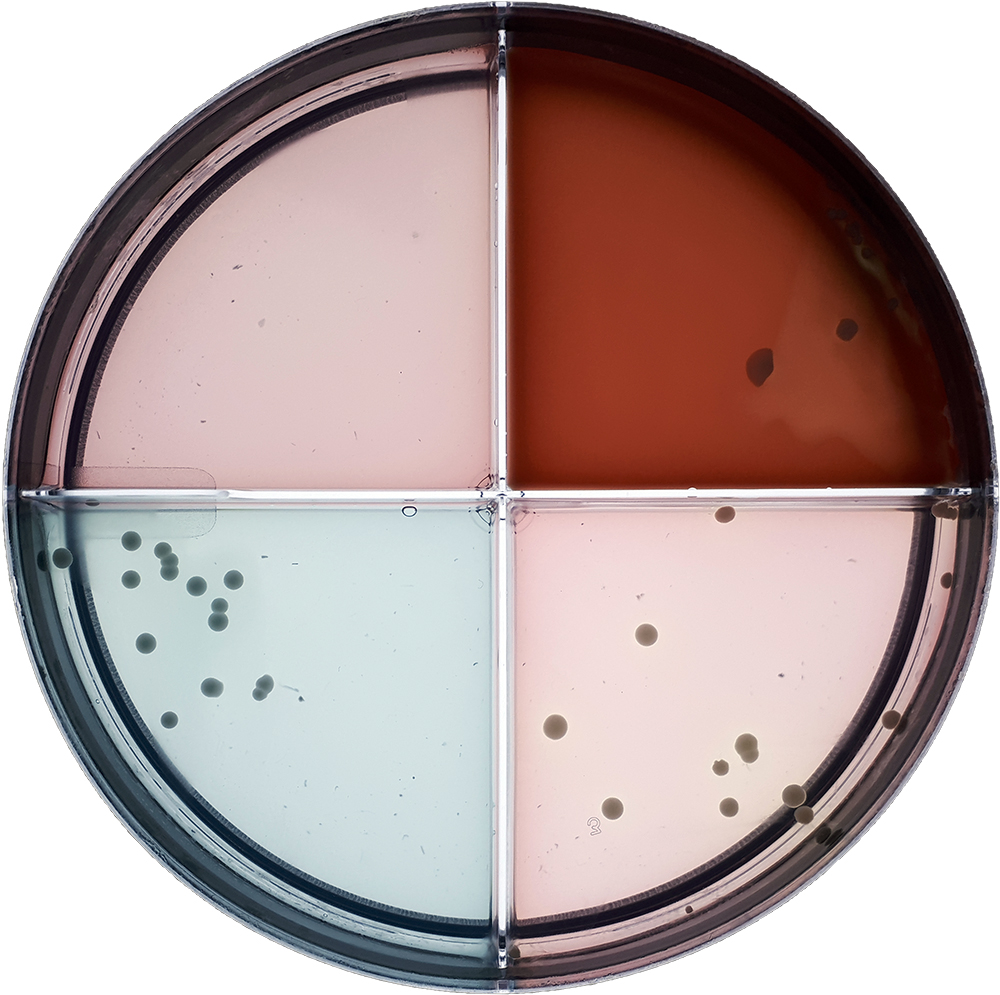
\includegraphics[width=0.40\linewidth]{figures/firstpage1.jpg}\\\\
\\\\\\\\
 Image Processing for\\ Improved Bacteria Classification}
\thesissubject{Computer Science}

\publicationyear{2020}
\currentyearthesisnumber{001}


\author{\parbox{\textwidth}{Emil Bråkenhielm (emibr678) \\ Peder Leijonhufvud (pedle936)}}
\begin{document}
\chapterstyle{VZ43}
\chapter{Introduction}
Mastitis is the most common disease among cows in dairy farms in Sweden\footnote{\url{http://intervacc.se/forskning-utveckling/projekt/novel-antigen/om-s-aureus/}}. Aside from great suffering for the animals, mastitis is very costly for agriculture and contributes to the use of antibiotics. As an example, the cost per mastitis in Sweden approximates to be over 3300 SEK due to treatment cost and reduced milk production. Furthermore, there are approximately 380 000 milk cows in Sweden, and 75 000 of these cows are treated annually with antibiotics due to mastitis. Mastitis is caused by, in most cases, bacterial infection, and it is therefore important to get a diagnosis as soon as possible to know what kind of bacteria it is. \\ 

\noindent Today, most cases of mastitis are diagnosed by licensed veterinarians or specially trained laboratory technicians\footnote{\url{http://www.juverportalen.se/media/1176/mastitdiagnostik-naer-var-hur.pdf}} who analyze bacteria growth on agar plates. However, this is both time-consuming and expensive for the farmer. \\

\noindent Bacteria classifiers are currently in development to automate the whole process by analyzing images of agar plates. However, the classification today is dependent on the conditions and quality of the image. A too large difference between the images may result in faulty diagnostics. The input images, therefore, need to be properly pre-processed using image processing to address any variety in scale, positioning, perspective, illumination, and noisy backgrounds.  

%If a cow is suspected of carrying the infection, a milk sample is sent to a bacteriological laboratory for examination.  The complexity of the diagnosis process makes it less likely that the farmer will identify the infection in an early stage, thus increasing the chance of clinical mastitis.

\section{Motivation}
Agricam is an IT-company located in Linköping who develops products and services adapted for dairy farmers. The company aims to streamline and digitalize animal health work. They are currently developing a bacteria classifier to automatically identify mastitis bacteria in milk samples from Swedish dairy farms. \\

\noindent Bacteria samples for mastitis are usually collected from each teat of an udder. The agar plate for this type of bacteria growth is thereby divided into four compartments. Each compartment corresponds to a specific quadrant of the udder, which helps to localize the infection. \\

\noindent The rotation of the agar plate is thus of great importance to not confuse any sample with the wrong part of the udder. To distinguish between the compartments, the agar in each compartment has different colors. Which color corresponds to what udder part, however, are not identified by the classifier.\\

\noindent Therefore, each sample image needs to be pre-processed to ensure correct rotation. Variety in scale, position, perspective, and illumination may also affect the diagnosis. So by defining a model in terms of previously mentioned factors, each image can be processed to fit the model, consequentially leading to correct rotation and higher diagnostic accuracy.

%\noindent For an optimized bacteria classification, the agar plate must be positioned correctly in every picture. A correct position also applies to the rotation of agar plates with its compartments. \\

%\noindent Previous work on automated bacteria detection exists. \cite{Minoi} states that without proper image pre-processing, a bacteria classifier may only be reliable under controlled environments. 

%Therefore, to make a bacteria classifier more reliable in uncontrolled environments, each input needs to be pre-processed considering the variety in scale, positioning, lighting, perspective, and noisy backgrounds.

\section{Aim of the work}
This thesis aims to investigate if a combination of image processing techniques can pre-process images of agar plates to be positioned correctly despite variations in scale, positioning, lighting, perspective and noisy backgrounds. 

\section{Problem description}
\begin{enumerate}
  %  \item Hur kan man på bästa sätt identifiera odlingsplattan och de fyra fälten i bilderna med hjälp av bildbehandling och/eller machine learning?
    \item Investigate if a combination of image processing techniques can be used for scale, rotation, and perspective invariant image registration of agar plates, based on the criteria below. 
    
    %before: find a combination of image processing techniuqes for... 
\end{enumerate}
\textbf{Criteria:} 
\begin{enumerate}
    \item The outer edge of the agar plate shall be identified. The compartment edges shall be identified as well. 
    \item Pixels outside the agar plate should be masked to remove background noise.
    \item Depending on the angle, rotation, position, and scale, the image should be adjusted to match a reference picture.
\end{enumerate}

%This thesis aims to investigate if an combination of image processing techniques can optimize 
%This thesis aims to investigate if an combination of image processing techniques can optimize the input images for Agricams bacteria classifier. The agar plate should be position correctly despite, the rotation, perspective, angle and scale to begin with. 
%\noindent To solve these problems and to improve the bacteria classifier's output, this thesis will i§nvestigate how to optimize the input images using different image processing techniques.

%This thesis aims to investigate if an combination of image

%Though the current solution of the bacteria classifier is based on a controlled environment using the customized stand. The thesis aims to find an approach that is not only optimized for these conditions but to improve the reliability even in uncontrolled environments.

\section{Limitations}
The following limitations have been taken during the work: 
\begin{enumerate}
    \item Images used should be with high enough resolution and quality to distinguish each bacteria cluster. Correction of image deviations may also be limited to the extent that the image quality needs to be good enough for the classifier. Too extreme variations may, therefore, be dismissed. 
    %The classifiers limit the definition of an uncontrolled environment; in this case, the need for images with high enough resolution to distinguish each bacteria cluster. Correction of image deviations may also be limited to the extent that the image quality needs to be good enough for the classifier. Too extreme variations may, therefore, be dismissed.
\end{enumerate}


%\nocite{scigen}
%We have included Paper \ref{art:scigen}

%%%%%%%%%%%%%%%%%%%%%%%%%%%%%%%%%%%%%%%%%%%%%%%%%%%%%%%%%%%%%%%%%%%%%%
%%% Intro.tex ends here

%%% Local Variables: 
%%% mode: latex
%%% TeX-master: "demothesis"
%%% End: 


%%% lorem.tex --- 
%% 
%% Filename: lorem.tex
%% Description: 
%% Author: Ola Leifler
%% Maintainer: 
%% Created: Wed Nov 10 09:59:23 2010 (CET)
%% Version: $Id$
%% Version: 
%% Last-Updated: Tue Oct  4 11:58:17 2016 (+0200)
%%           By: Ola Leifler
%%     Update #: 7
%% URL: 
%% Keywords: 
%% Compatibility: 
%% 
%%%%%%%%%%%%%%%%%%%%%%%%%%%%%%%%%%%%%%%%%%%%%%%%%%%%%%%%%%%%%%%%%%%%%%
%% 
%%% Commentary: 
%% 
%% 
%% 
%%%%%%%%%%%%%%%%%%%%%%%%%%%%%%%%%%%%%%%%%%%%%%%%%%%%%%%%%%%%%%%%%%%%%%
%% 
%%% Change log:
%% 
%% 
%% RCS $Log$
%%%%%%%%%%%%%%%%%%%%%%%%%%%%%%%%%%%%%%%%%%%%%%%%%%%%%%%%%%%%%%%%%%%%%%
%% 
%%% Code:



\chapter{Theory}
The following chapter describes the necessary information needed to solve the problem description and to help design an appropriate method. The theoretical part will first explain the concept of an agar plate, followed by various existing approaches to image processing and edge identification. 
\\

\section{Agar Plate}
Agar plates are Petri dishes containing agar, which is a gelatinous substance derived from red algae used as a bacteria growth medium. Agar plates are often used in laboratory settings to analyze if certain bacteria exist within a sample. Depending on the situation, the agar plate could be divided into multiple compartments, as shown in \textit{Figure \ref{fig:agar plate}}. Each compartment can be used to test different samples or the same sample with different bacteria.


% to reference a figure \ref{label}

%\begin{figure}[H]
%  \includegraphics[scale=1.7]{birds.jpg}
%  \caption{The birds}
%  \label{fig:birds}
%\end{figure}
    \begin{figure}[H]
        \begin{center}
            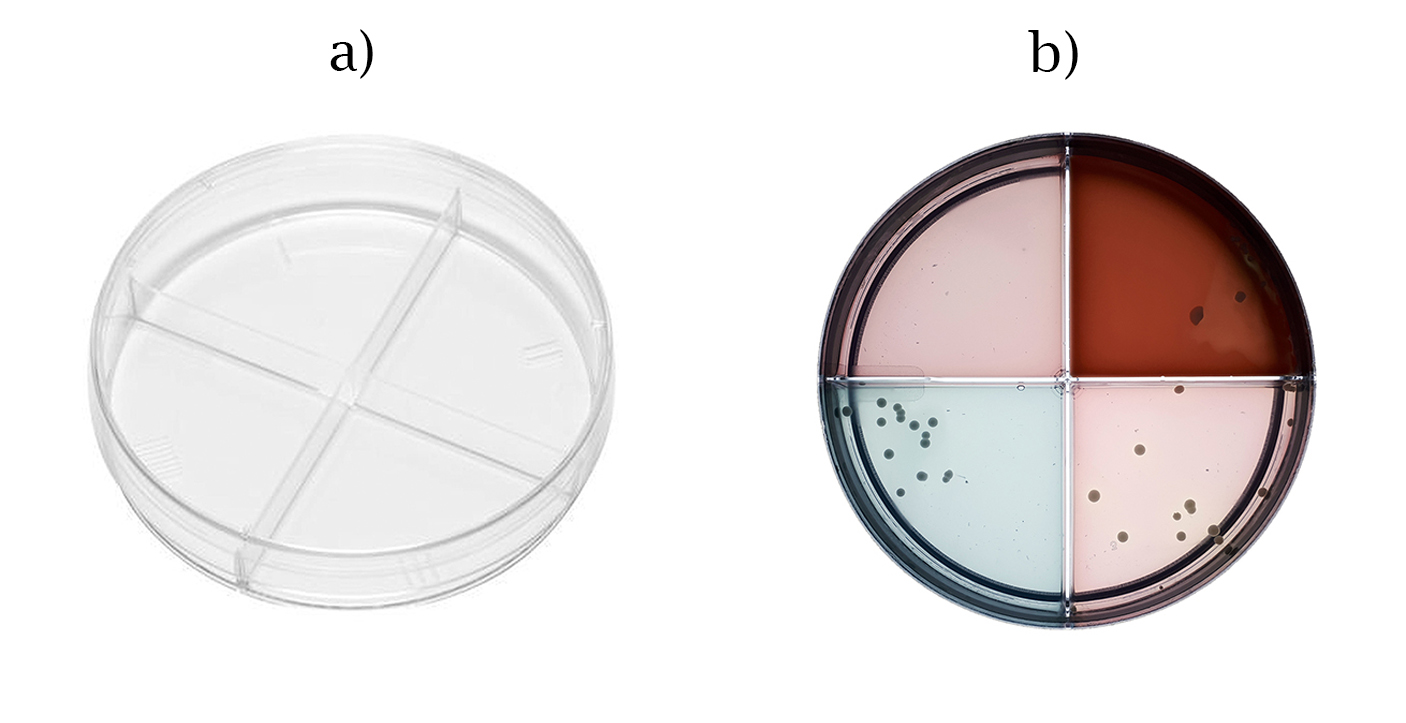
\includegraphics[width=.7\linewidth]{figures/petri.jpg}\\
            \caption{ a) Empty Petri dish with four compartments. b) Petri dish with agar, i.e., an agar plate.}
            \label{fig:agar plate}
        \end{center}
    \end{figure}

\section{Image Processing}

\noindent Digital image processing is about manipulating pixels. For example, improving, analyzing, or in some way, extracting information from an image. This section will focus on this type of algorithms and techniques, focusing on techniques suitable for the aim of the work.

%\section{Brightness and contrast}
\subsection{Color correction}
Altering the color of an image is an essential task in image processing and often means removing a dominant and undesirable color in a picture. Objects may have different colors on the images compared to reality. \\

\noindent \cite{Limare} proposes a color balance algorithm named Simplest Color Balance (SCB). The algorithm works by stretching red, green, and blue values within a [0, 255] range. High values are assumed to be white, and low values black. An image with low brightness, for example, may not have any pixels close to 255. By stretching the color scale [0, 255], the brightness can be increased or decreased. 


\subsection{Edge detecting}
\noindent Edges (i.e., an abrupt change of gray or color intensity) need to be distinguished in order to extract specific data of objects in images. By minimizing the number of false edges, often caused by image noise,  actual edges could easier be identified. If the goal is to find the most intense edge, as the edge of an agar plate, blur filters and morphological operations could be used as an extension. The Hough Transform algorithm (see \textit{Section 2.2.2.6}) is designed to find simple shapes within an image and to extract the coordinates or the area of an object.



\subsubsection{Canny Edge Detection}
The Canny operator\cite{Xuan} is based on a multi-stage algorithm initially developed to detect edges in images. Canny is divided into five different stages explained below. \\

\noindent \textbf{Gaussian Blur}\\
The first stage of Canny is to apply a Gaussian blur filter to reduce any image noise occurring, as shown in \textit{Figure \ref{fig:gaussian blur}}. Otherwise, pixel noise could be falsely detected as an edge. The algorithm uses a kernel, which is a convolution matrix of $n*n$ pixels, to search all pixels in an image. Each pixel is evaluated, and its pixel value is replaced with a weighted mean of its neighboring pixels. A two-dimensional Gaussian function is generally used to remove image noise (see \textit{Equation 2.1}). \begin{equation} G(x,y)=exp[-(x^2+y^2/2\sigma^2]/2\pi\sigma^2\end{equation} Where $\sigma$ (sigma) is the parameter that controls the smoothing extent of an image. 

\begin{figure}[H]
        \centering
        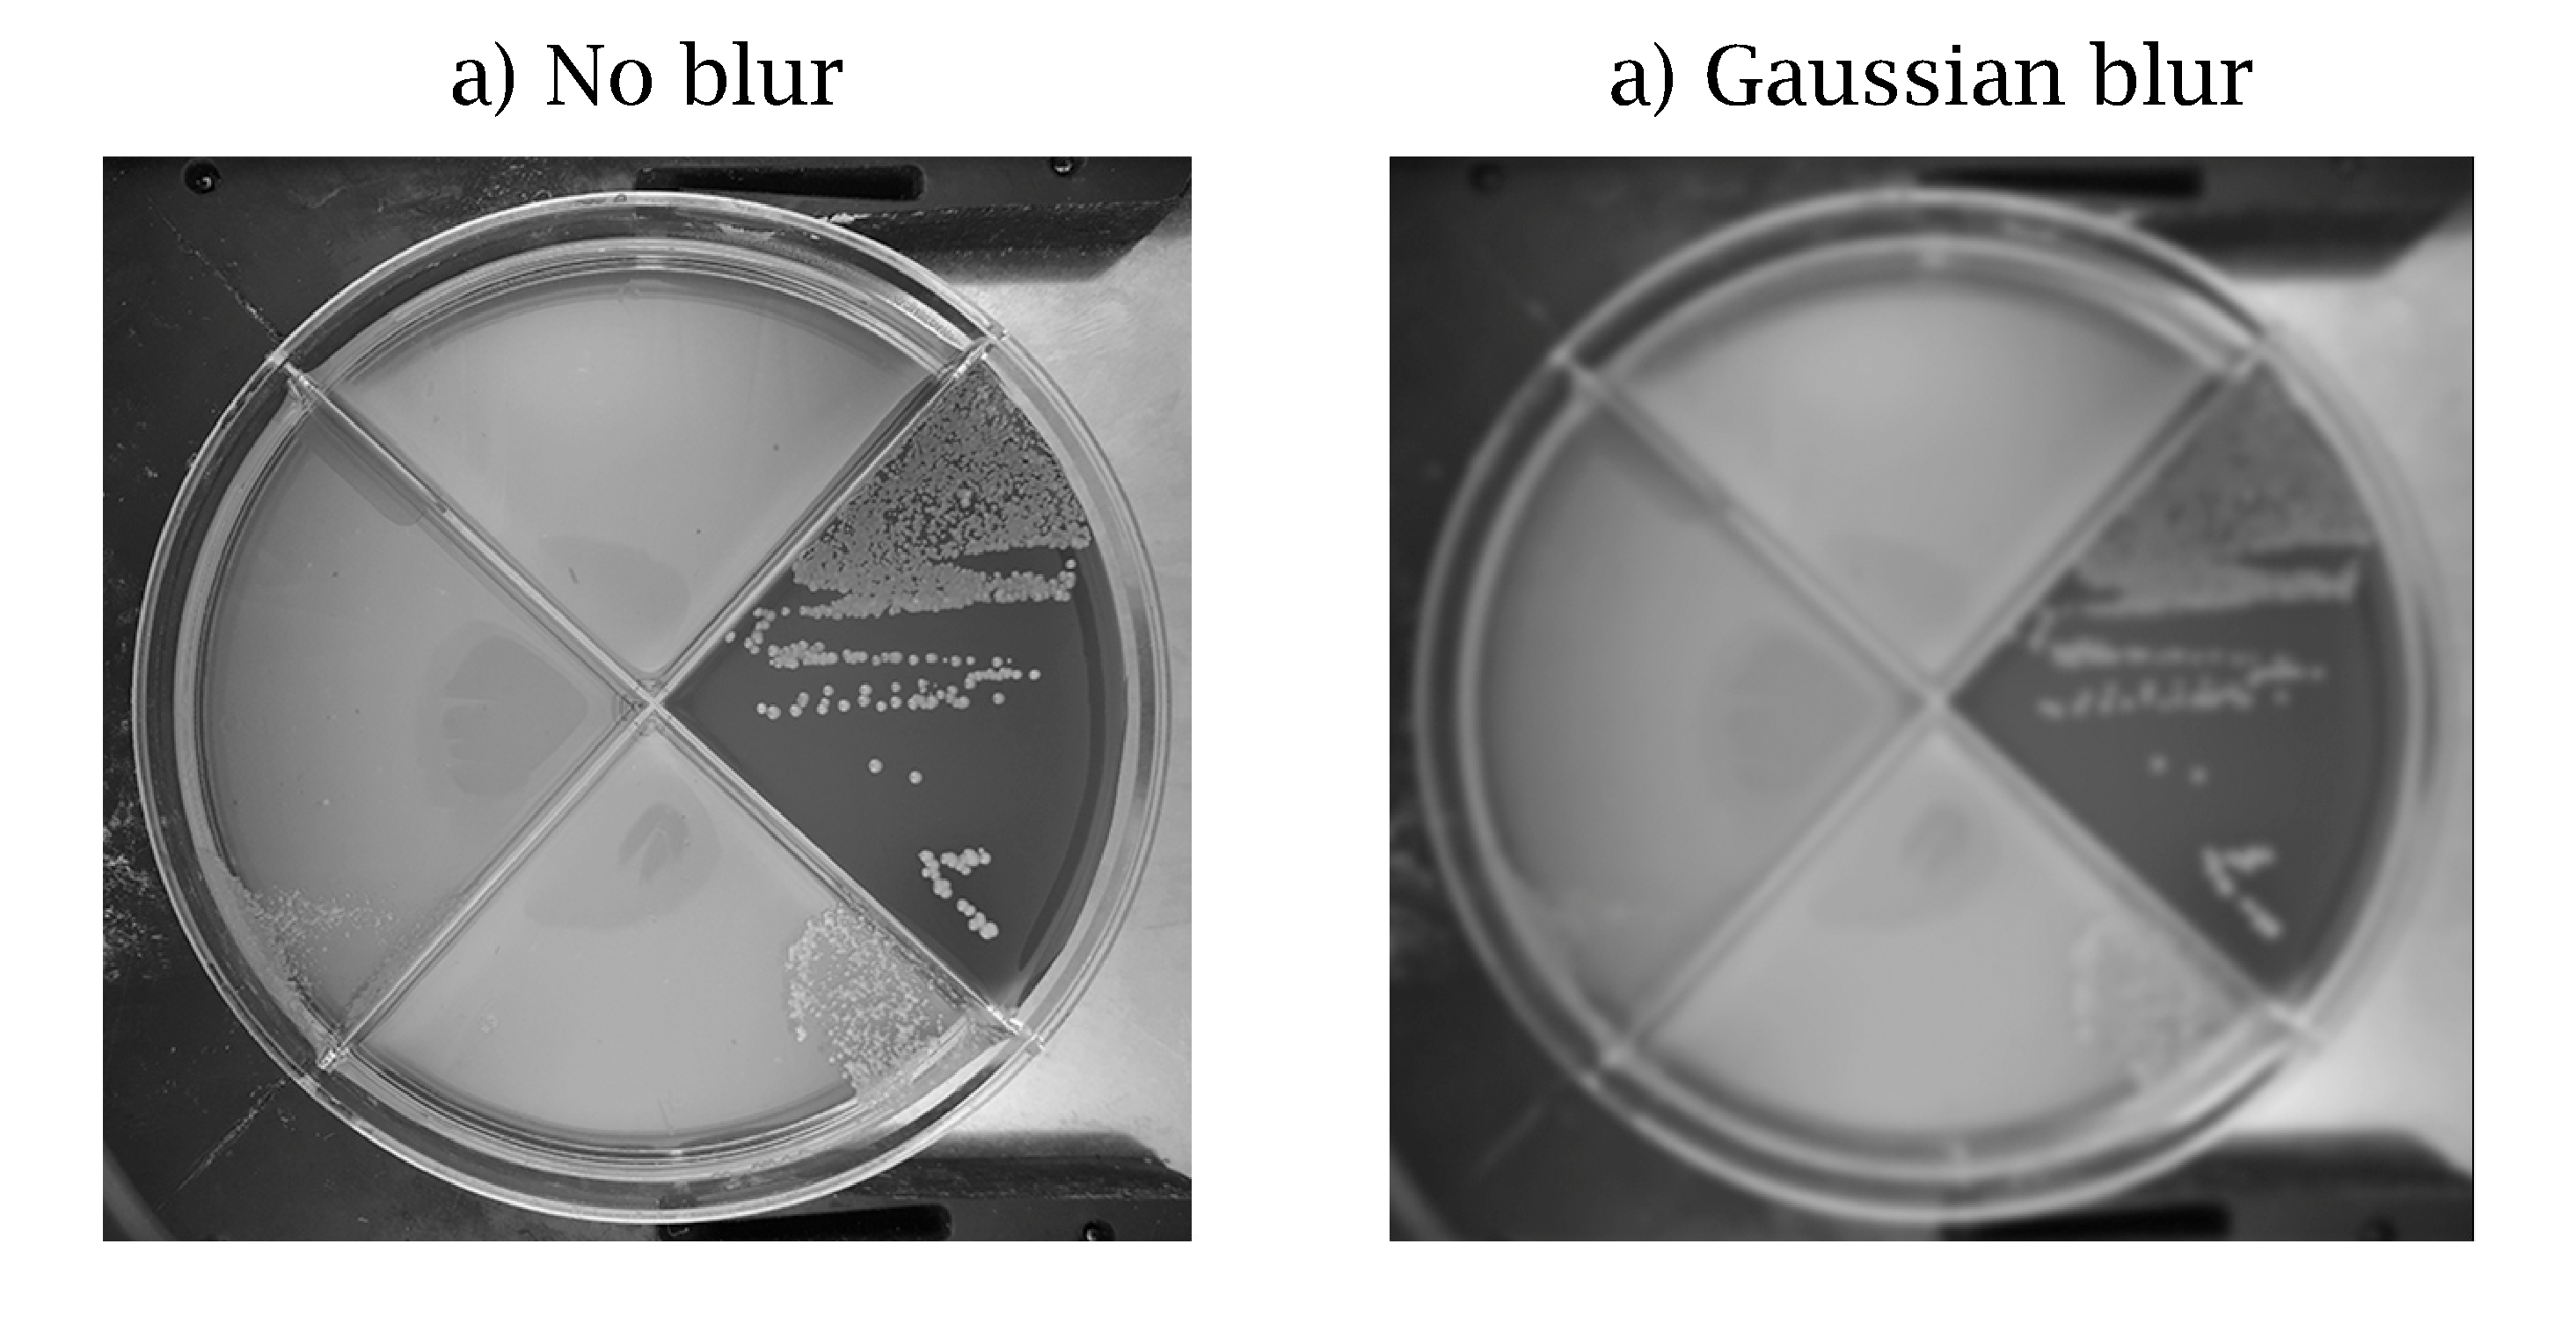
\includegraphics[width=.7\linewidth]{figures/PDF/Gaussian_blur.pdf}\\
        \caption{a) Before applying Gaussian Blur. b) After applying Gaussian Blur}
        \label{fig:gaussian blur}
\end{figure}\\

\noindent \textbf{Sobel Operator}\\
\noindent After the applied blur, a Sobel kernel is used to identify all intensity gradients. With its kernel, Sobel looks for areas in the image that have a high gradient, i.e., a distinct and sudden change in color (in RGB) or brightness (in grayscale). \textit{Figure \ref{fig:sobel kernel}} shows how the method works in the x-axis as well as the y-axis. Each value within the kernel is multiplied by the value at the corresponding location in the image. The sum of the matrix gives a gradient value. A higher value means a more defined edge. The derivative of the respective edges is then calculated to determine the angle of the edge.\\

\begin{figure}[H]
        \centering
        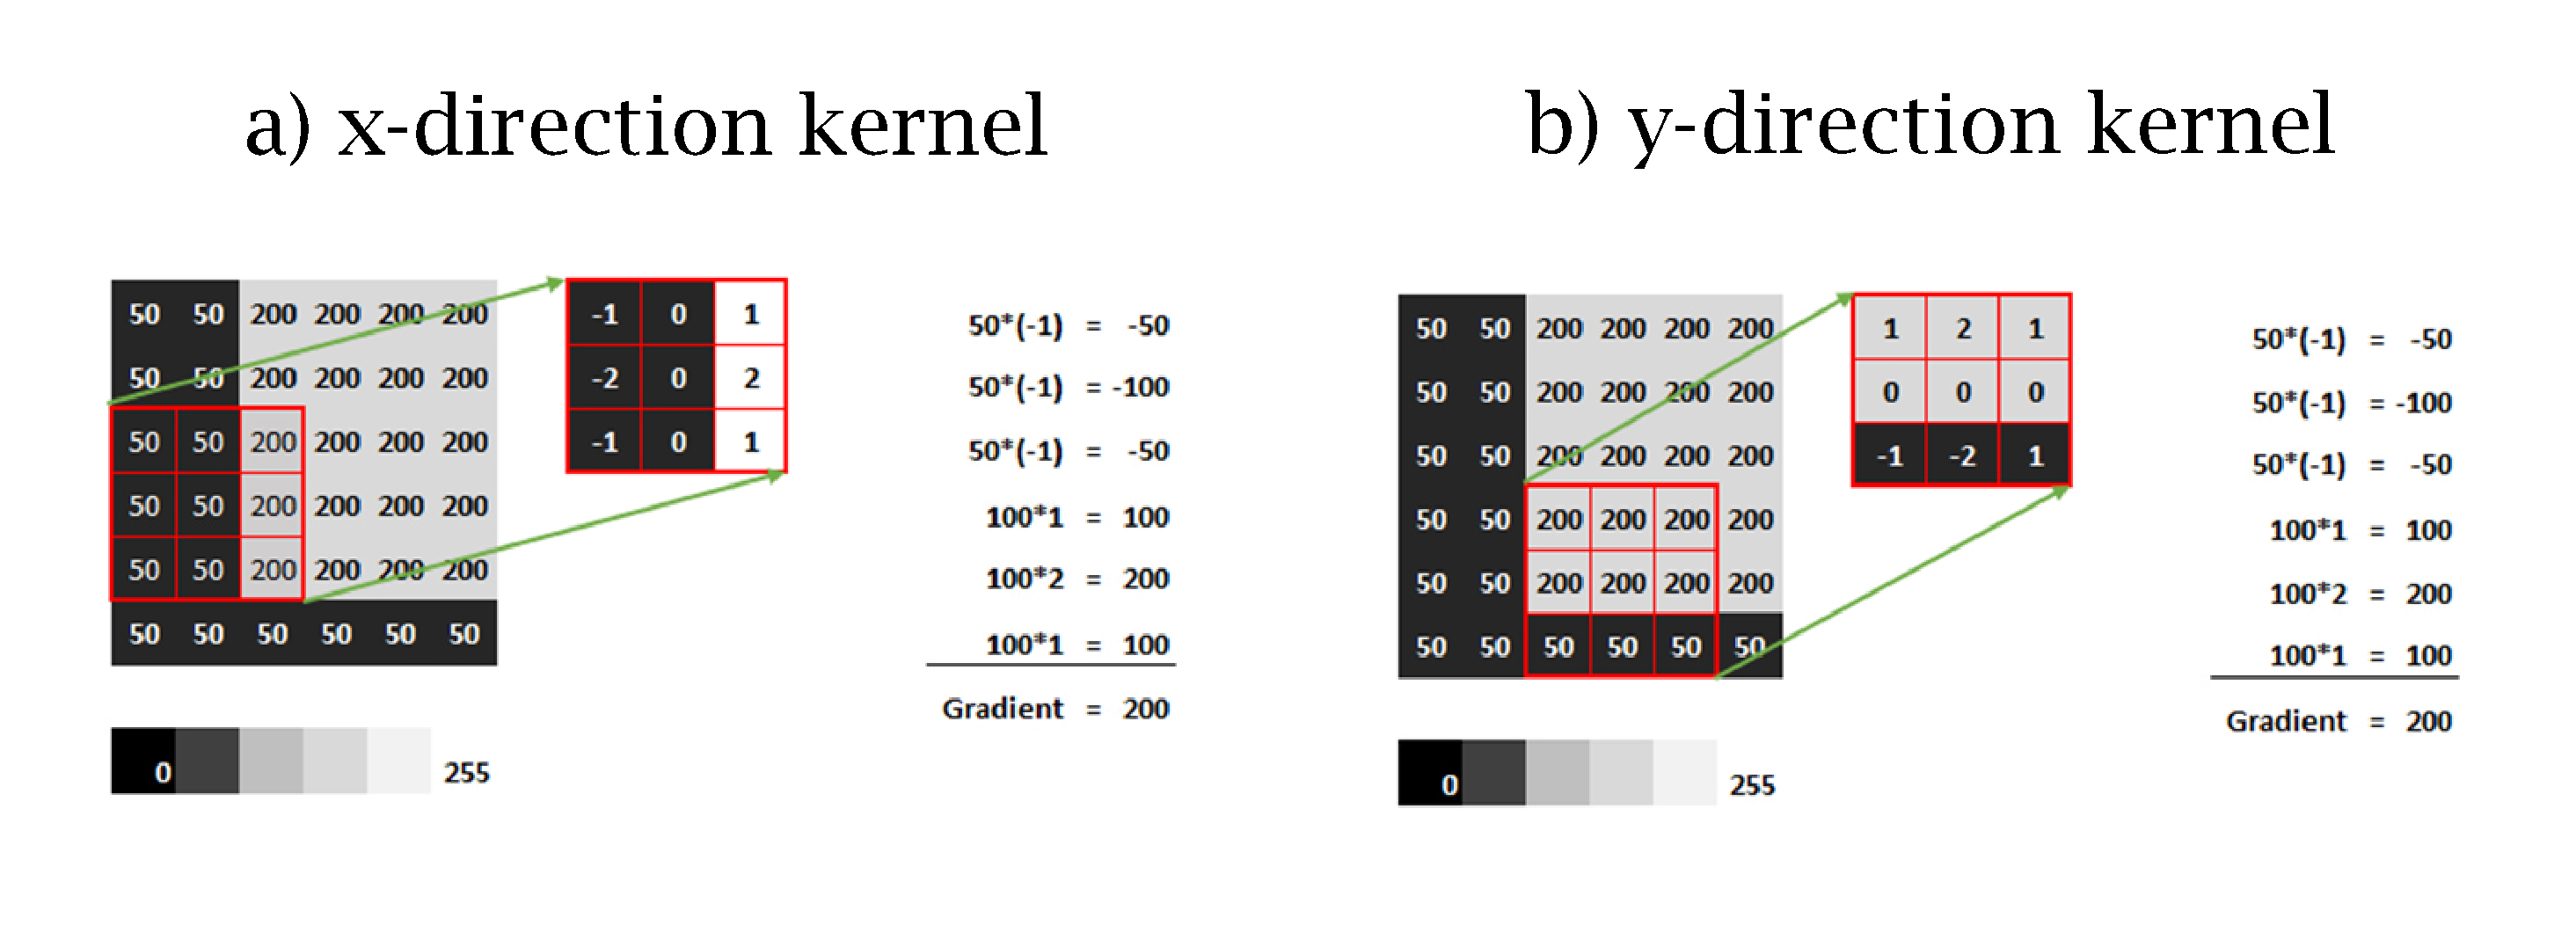
\includegraphics[width=1\linewidth]{figures/PDF/Sobel_kernel.pdf}
        \caption{The Sobel y-kernel checks for the gradient on the y-axis}
        \label{fig:sobel kernel}
\end{figure} \\\\

\noindent \textbf{Non-maximum suppression}\\
\noindent While the Sobel filter finds most edges, usually, only the most prominent are interesting. The output may have both thick and thin edges, and a non-maximum suppression can be used to sort out any false edges. \\

\noindent By using the gradient intensity matrix determined in the previous step, the algorithm seeks through the image, following the direction of the edge. For each pixel, the algorithm checks neighboring pixels to the left and right of the edge. If a neighboring pixel in the same direction is more intense than the current pixel, the most intense pixel is kept. \textit{Figure \ref{fig:canny suppression}} shows an example where the pixels with intensity values 170 and 115 would be dismissed, and 255 kept.\\

\begin{figure}[H]
    \centering
     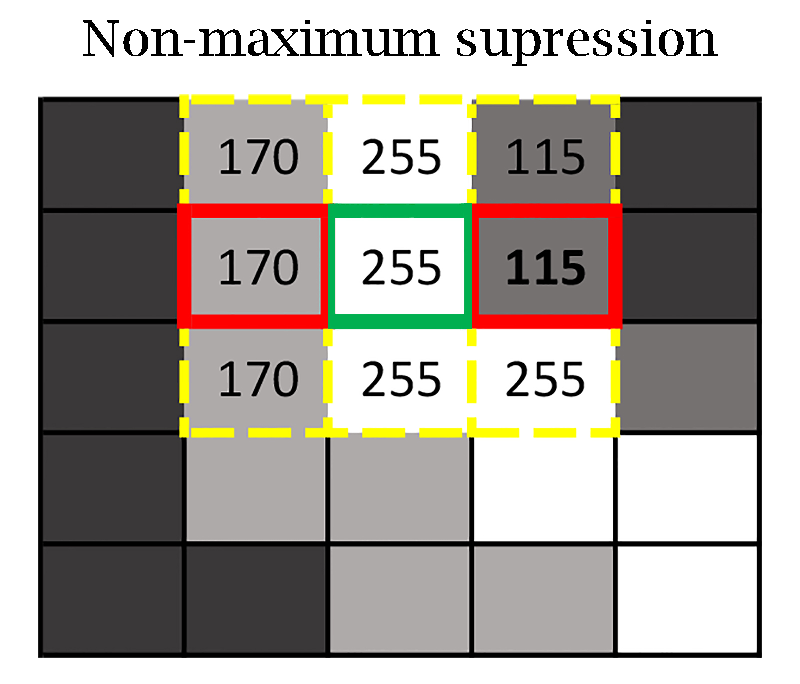
\includegraphics[width=.37\linewidth]{figures/PDF/Suppresion.pdf}\\
    \caption{Non-maximum suppression illustration. Values in red are dismissed, and green kept.}
    \label{fig:canny suppression}
\end{figure}

\noindent \textbf{Double threshold}\\
\noindent The non-maximum suppression will keep the most intense pixels identified in each edge, but there can still be intensity variations between these pixels. A lower and upper threshold is applied to strengthen the edge, which checks for pixels that are strong, weak, or non-relevant. The lower threshold is used to identify non-relevant pixels, while the upper threshold searches for strong pixels. Any pixels between the lower and upper threshold are marked as weak and will later be processed in the Hysteresis mechanism.\\ 

\noindent \textbf{Hysteresis}\\
\noindent The last stage of the Canny process is to decide which edges are true or not. With user-defined min and max parameters of a new threshold, previously detected weak pixels are transformed to strong pixels only if their pixel value is within the defined threshold range. \texit{Figure \ref{fig:hysteresis} b)} illustrates this procedure by discarding non-relevant pixels to value 0. The identified pixel also needs to be connected to a known edge, or else it will be discarded. \\

\begin{figure}[H]
    \centering
    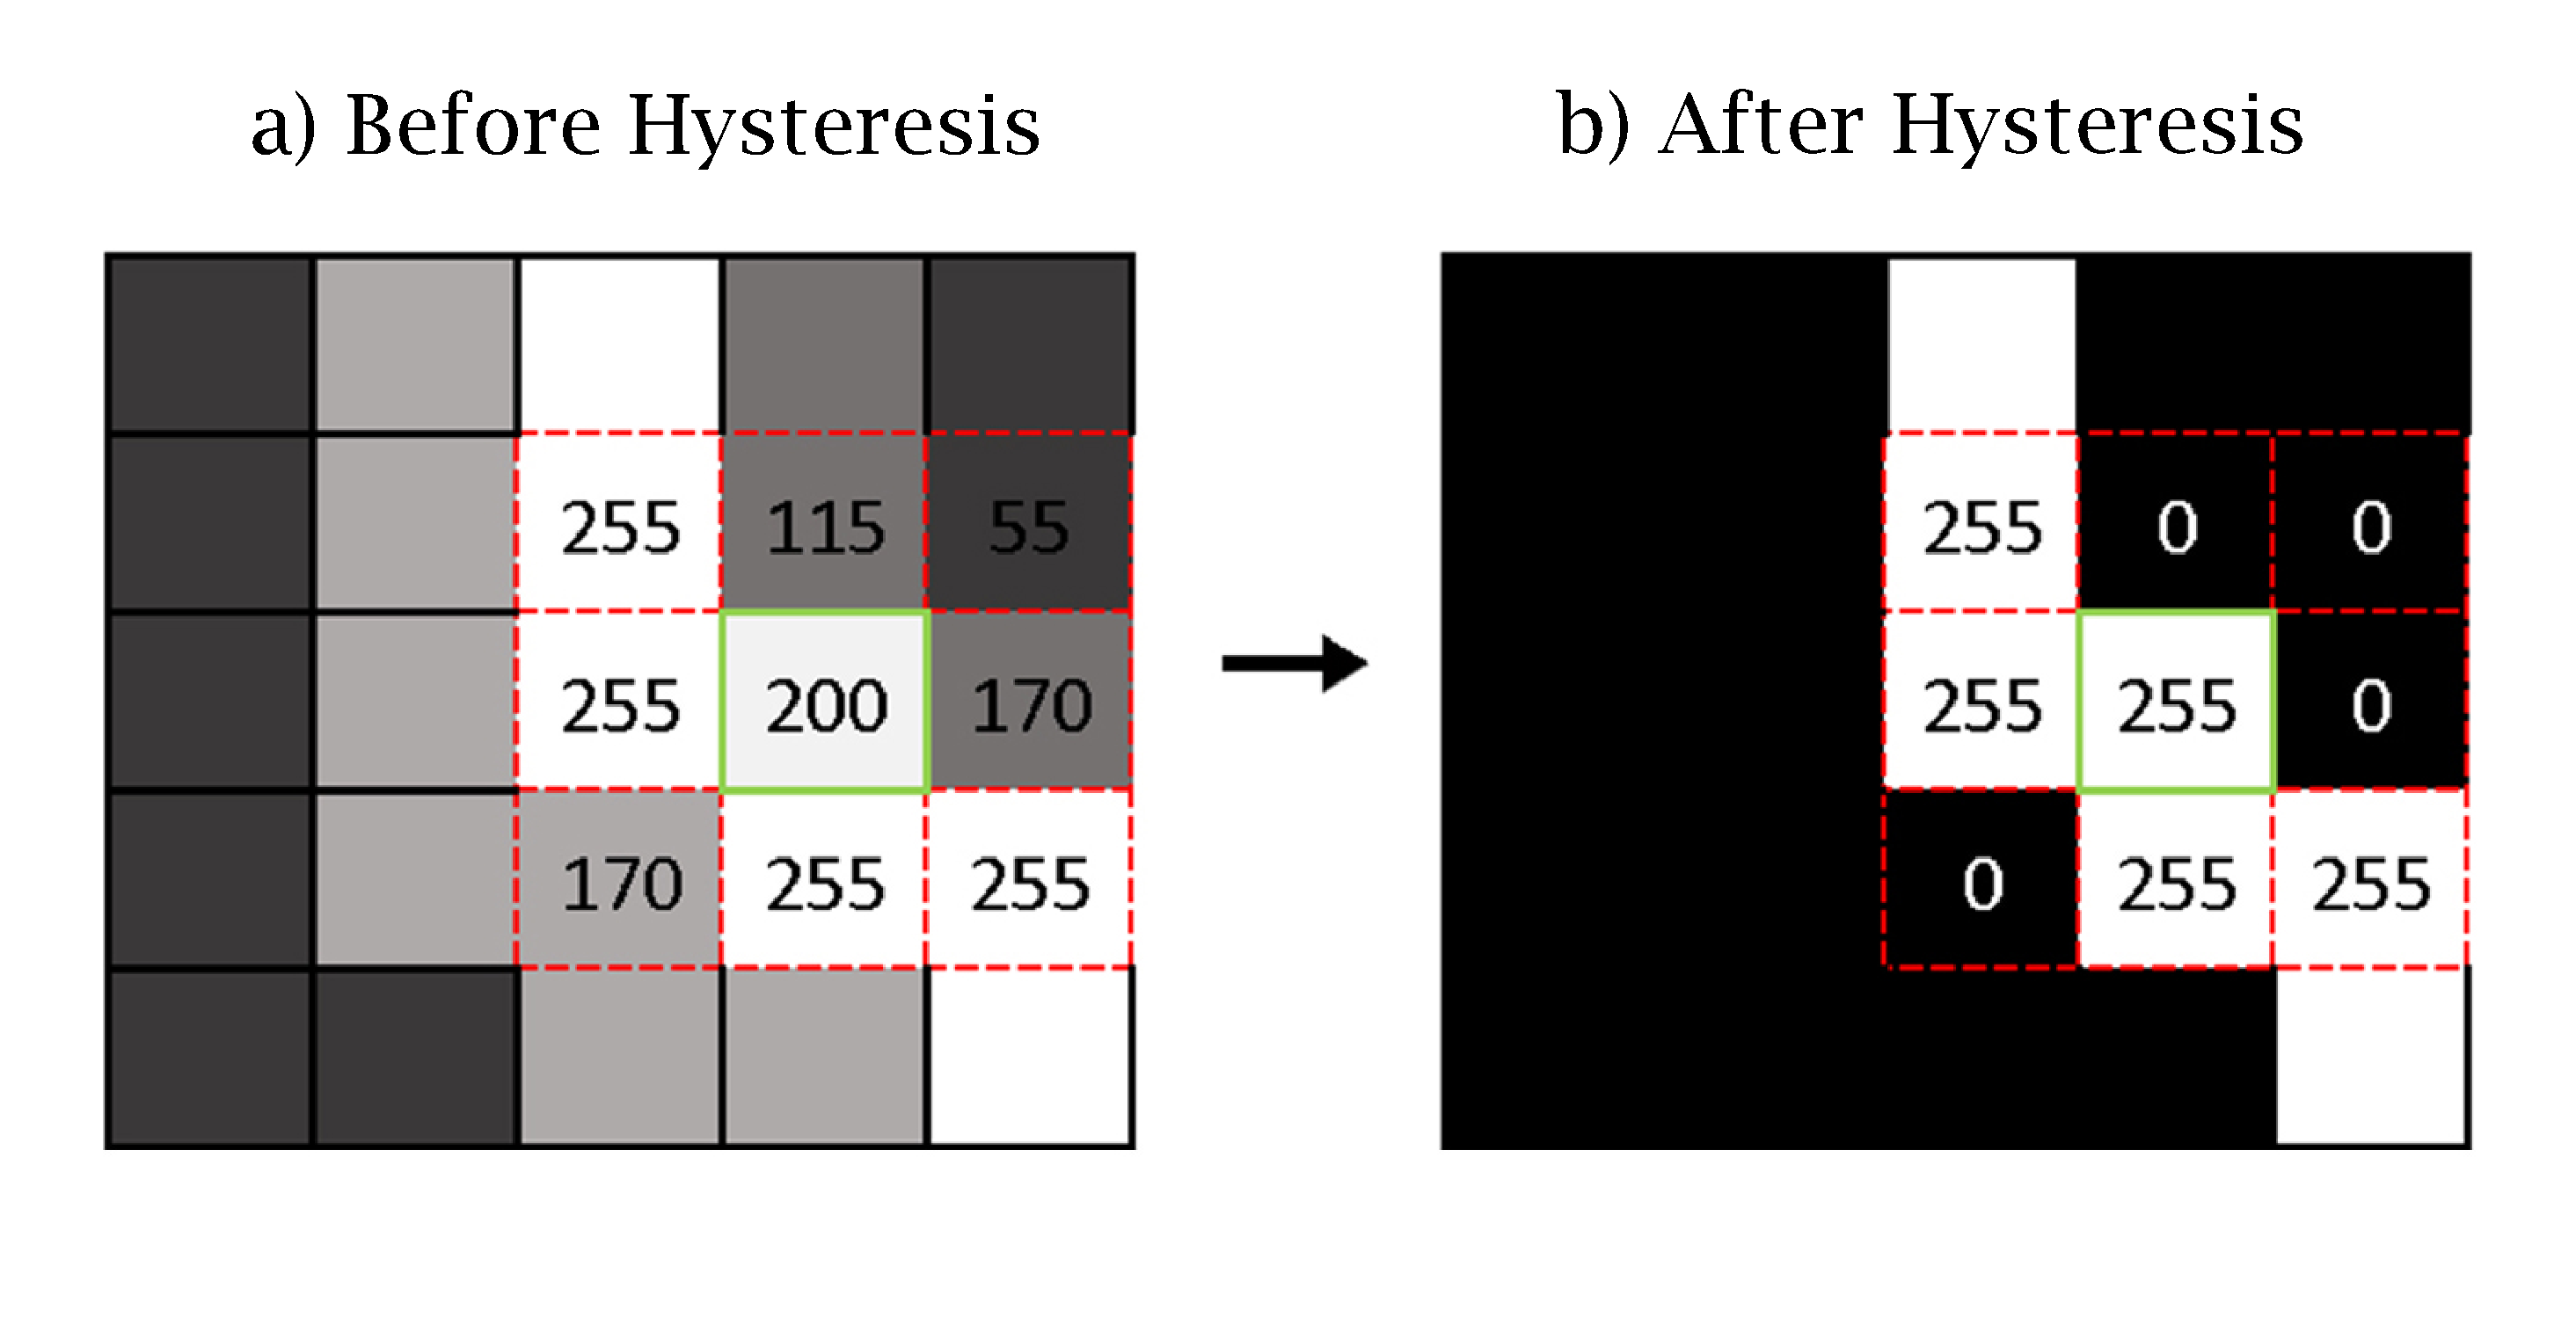
\includegraphics[width=.65\linewidth]{figures/PDF/Hysteresis.pdf}
    \caption{a) Before Hysteresis, b) after Hysteresis.}
    \label{fig:hysteresis}
\end{figure}

\subsubsection{Morphological Operations}
Morphological operations are used to process images based on geometrical structures. Different operations can be used to fix broken edges or areas within or outside the given boundaries of an object. The most common morphological operations are \textit{Dilation} and \textit{Erosion}\cite{Raid}, which either adds or removes pixels from an object contour. Dilation, followed by erosion, is called \textit{Closing}, which can be used to repair disconnected edges. Its counterpart \textit{Opening} are instead erosion followed by dilation can instead be used to reduce image noise \\

\noindent A structuring element (a matrix of user-defined size), searches the image checking each pixel with its corresponding neighbor (see \texit{Figure \ref{fig:dilate and erode}}). The value of each pixel within the structuring element is then decided based on different rules. For the dilation, each pixel is set to the most intense value found within the structuring element, while erosion sets each pixel values to the least intense. 

\begin{center}
\begin{figure}[H]
    \centering
    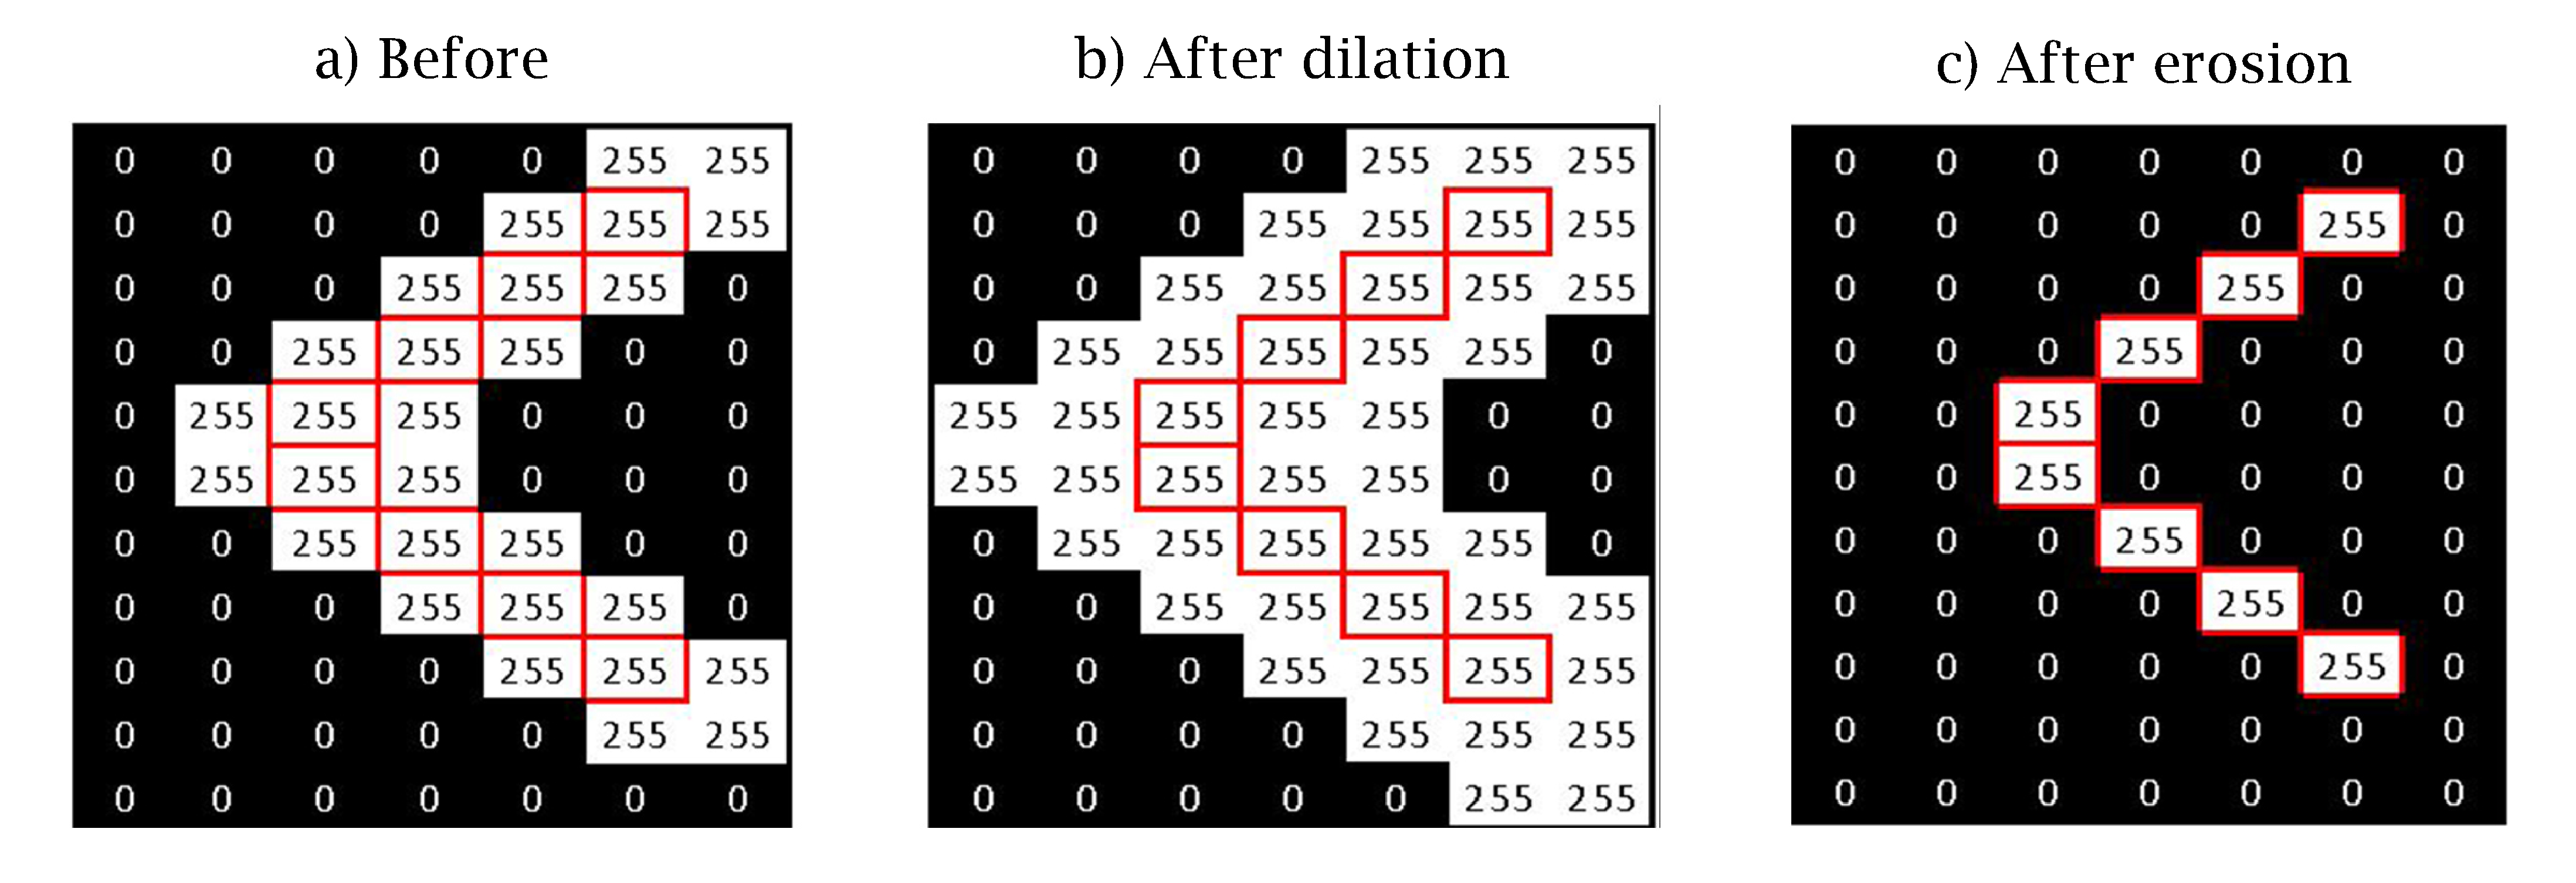
\includegraphics[width=1\linewidth]{figures/PDF/Morphological_dilate_erode.pdf}\\
    \caption{Dilation adds pixels to the object contour, while erosion
    removes pixels.}
    \label{fig:dilate and erode}
\end{figure}
\end{center}

\subsubsection{Skeletonize}
\textit{Skeletonization}\cite{Rakesh} is a technique that modifies a binary image using Dilation and Erosion to reduce foreground regions into a skeletal remnant, i.e., the innermost contour of a binary object (see \textit{Figure \ref{fig:skeletonize}}). In an ideal case, the result should give a 1-pixel-wide representation. By skeletonizing an image, one can achieve improved computation speed in image processing with only a light skeleton to process, as well as increased accuracy of finding the actual position of a line or edge.

\begin{figure}[H]
    \centering
    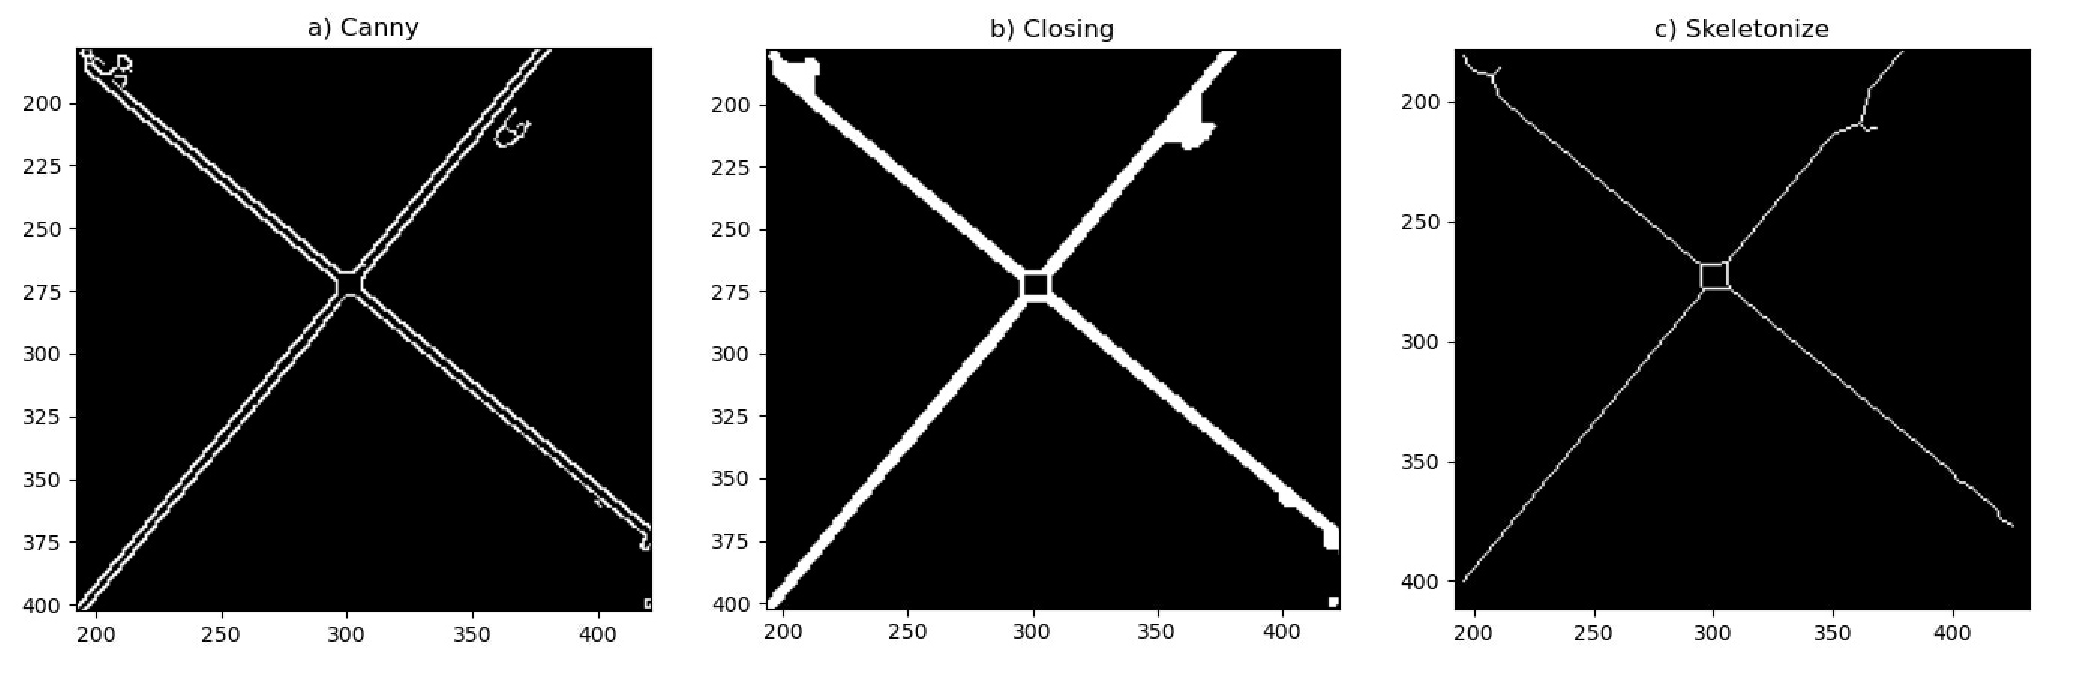
\includegraphics[width=0.8\linewidth]{figures/PDF/Skeletonize.pdf}\\
    \caption{The right image shows the output of a skeletonized binary image.}
    \label{fig:skeletonize}
\end{figure}

\noindent Opening is used to reveal the skeleton of an object. The process is repeated as long as the connectivity of the binary object is not broken. When broken, the last successful iteration is saved as output.

\subsubsection{Border following}
Extracting the contour of an object can be useful to analyze shapes and detect or recognize different objects. Border following \cite{Suzuki} is a type of algorithm that makes it possible to extract contours of given objects. Contours are generally defined by a closed curve joining the continuous points of an object boundary. For a contour to be identified, the object boundary should consist of pixels with the same color or intensity. 
For binary images, contours are divided into 1- and 0-components, which represent areas of their respectively binary image value. In \textit{Figure \ref{fig:suzuki border}}, $S_{1}$, which is the background 0-component, is interpreted as a hole between the frame border and the $B_{1}$ border. The algorithm checks images for 1-component and defines its borders as the transition between any 1-components neighboring 0-component.

\begin{figure}[H]
    \centering
     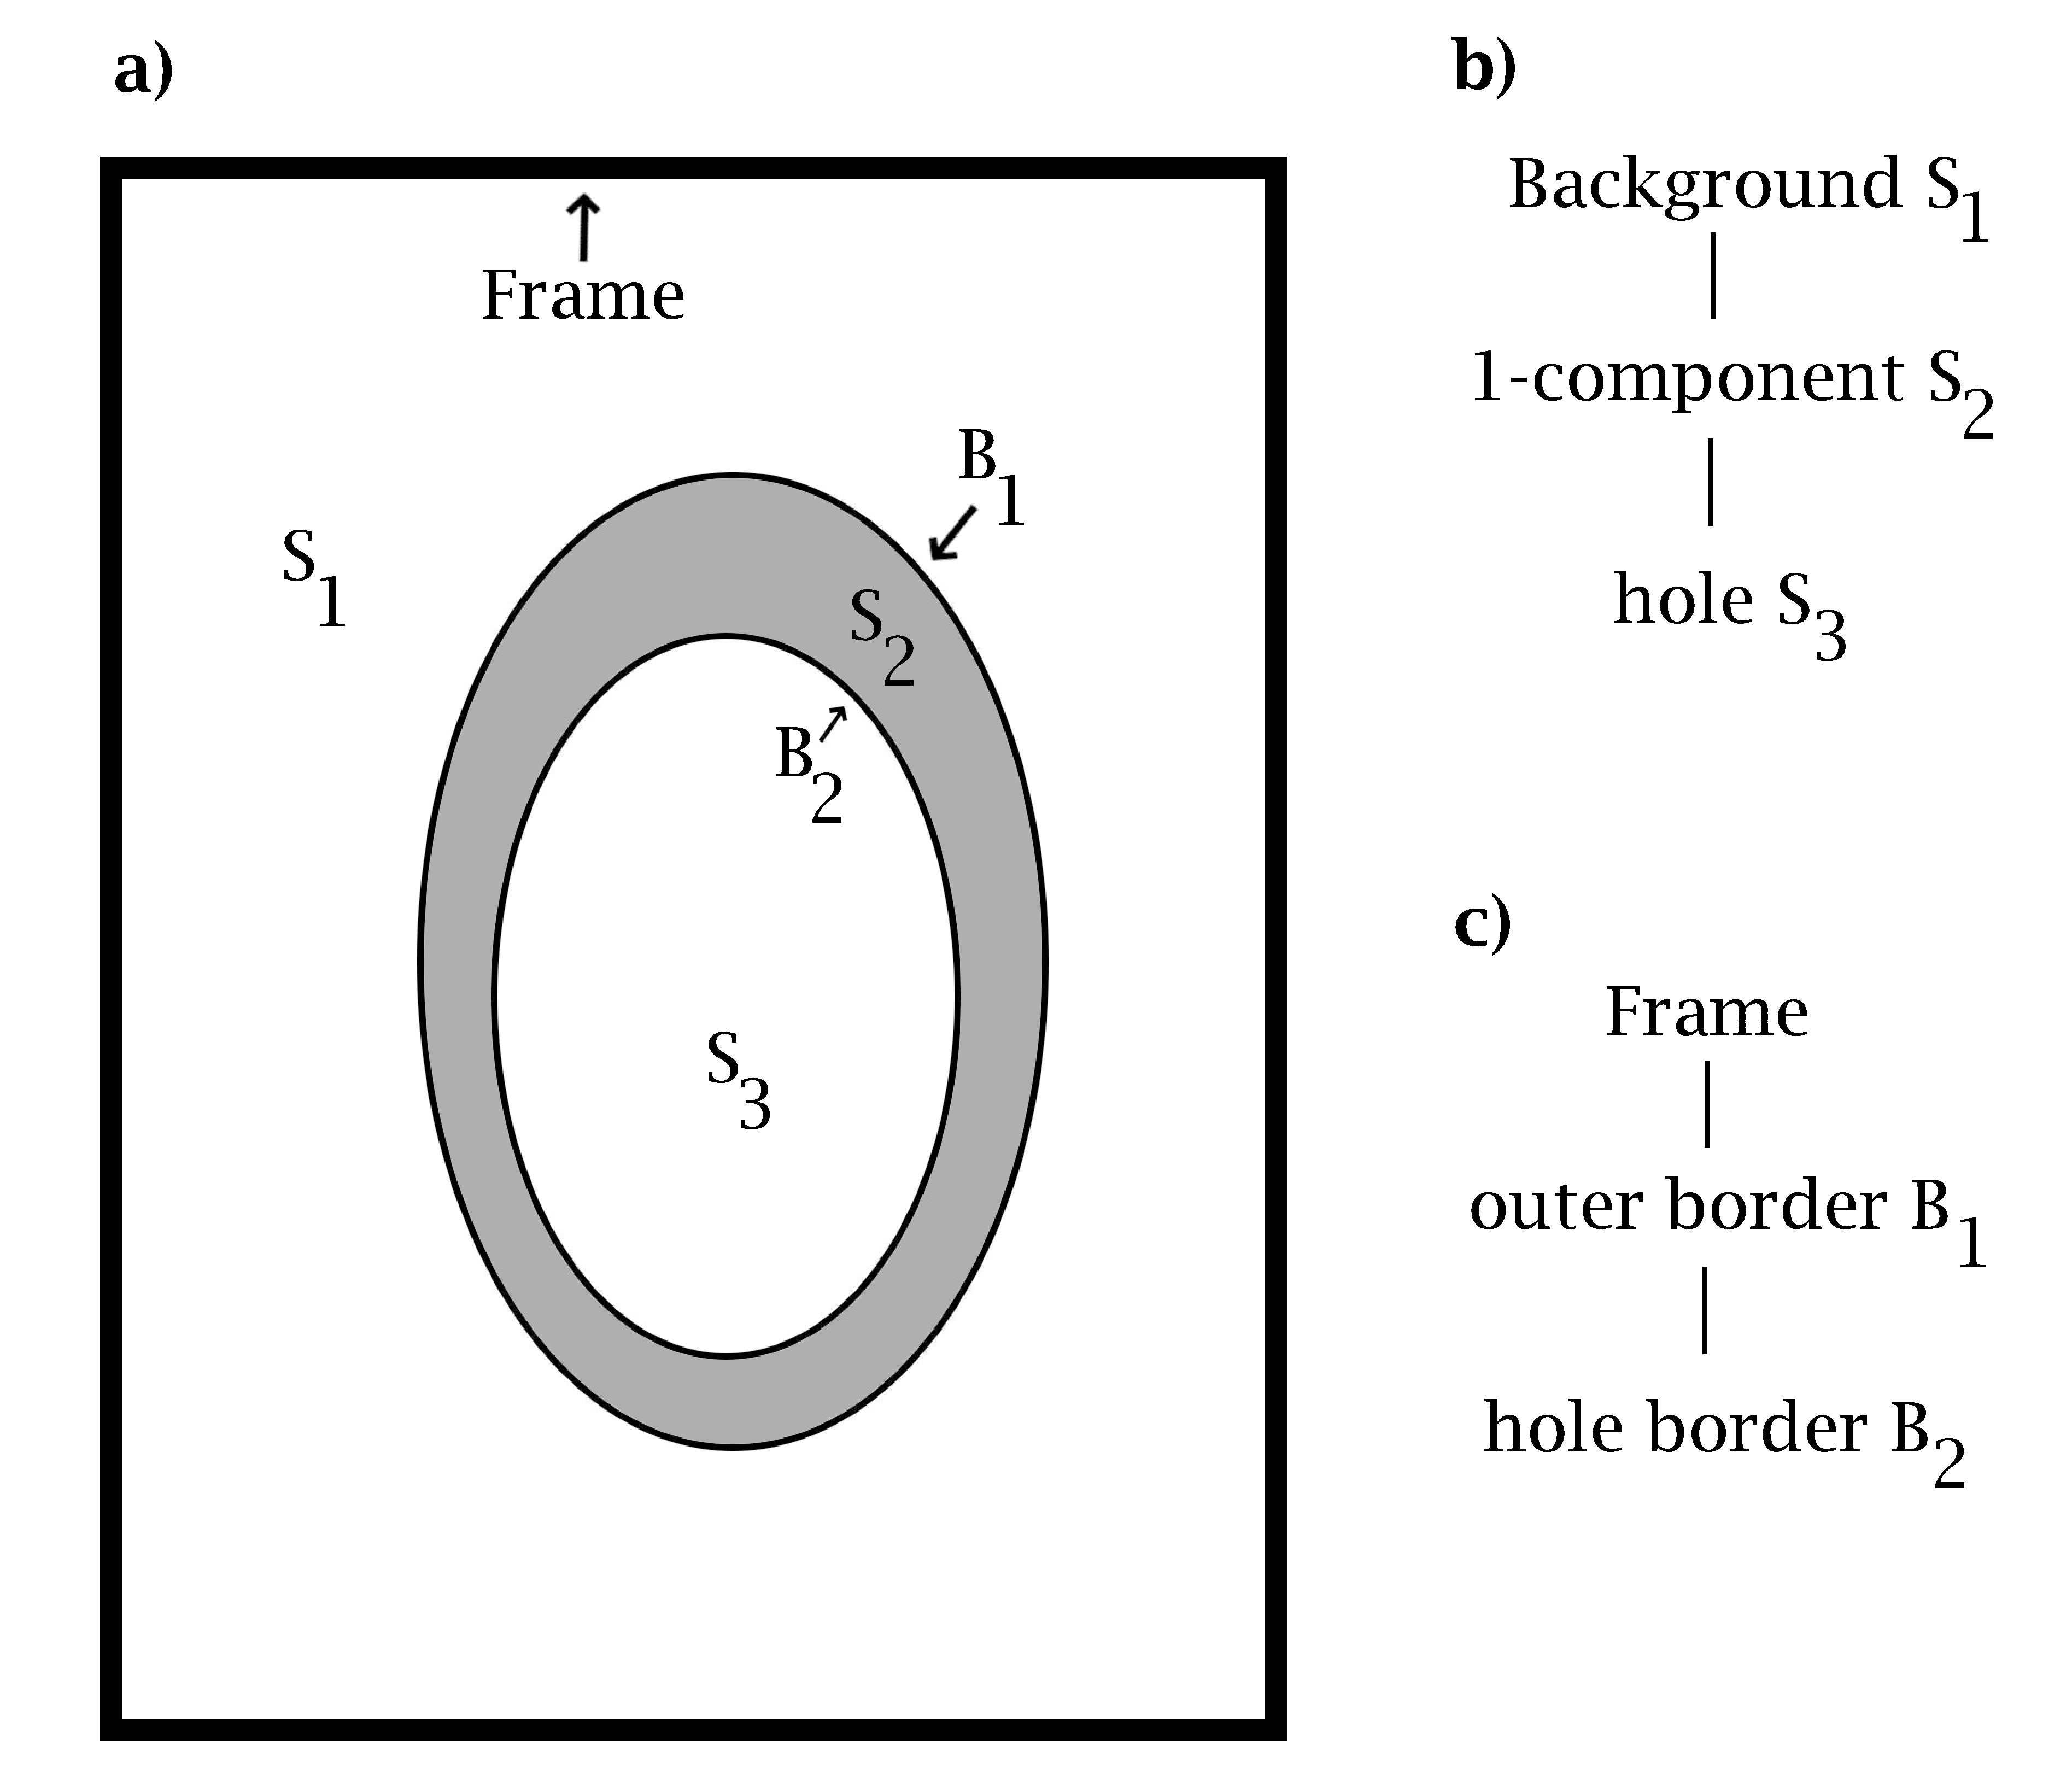
\includegraphics[width=0.65\linewidth]{figures/PDF/Border_following.pdf}
    \caption{a) Illustrates $S_{2}$ as a  1-component. b) Surroundness among components. c) Surroundness among borders (c)}
    \label{fig:suzuki border}
\end{figure}

\noindent Each contour found can be sorted into a different hierarchy based on length or occurrence moving outwards or inwards. A  child- and parent contour of a 1-component would occur in the same hierarchy. If a hierarchy level only consists of single contours, i.e., contours without a corresponding child or parent contour, that hierarchy level would return a negative value.  The external contour object of a single-object image could then be defined as being at the top of the hierarchy.\\

%\footnote{\url{https://docs.opencv.org/3.4/d3/dc0/group__imgproc__shape.html#ga17ed9f5d79ae97bd4c7cf18403e1689a}}
\subsubsection{Random Sample Consensus}
Random Sample Consensus (RANSAC)\cite{Fischler} is an algorithm used to estimate parameters of a given model. It is often used in Computer Vision to solve correspondence problems when defining what part of an image corresponds to in another image, i.e., feature matching.  The main idea is to cope with outliers occurring in input data, which is done by random sampling of observed data. The RANSAC algorithm can be configured to match specific shape models such as circles or ellipses, which can be useful to give a more accurate approximation of, e.g., a found contour.\\

\noindent \textit{Figure \ref{fig:ransac chart}} illustrates a simple least square method and a RANSAC approach for fitting a two-dimensional line. Both sets of observation contain inliers, i.e., points which can be approximated fitted to a line, and outliers which cannot be fitted. However, the least square method does not distinguish between outlier or inliers, and would, in this case, give a poor result.\\

\begin{figure}[H]
    \begin{minipage}{\textwidth}
        \centering
        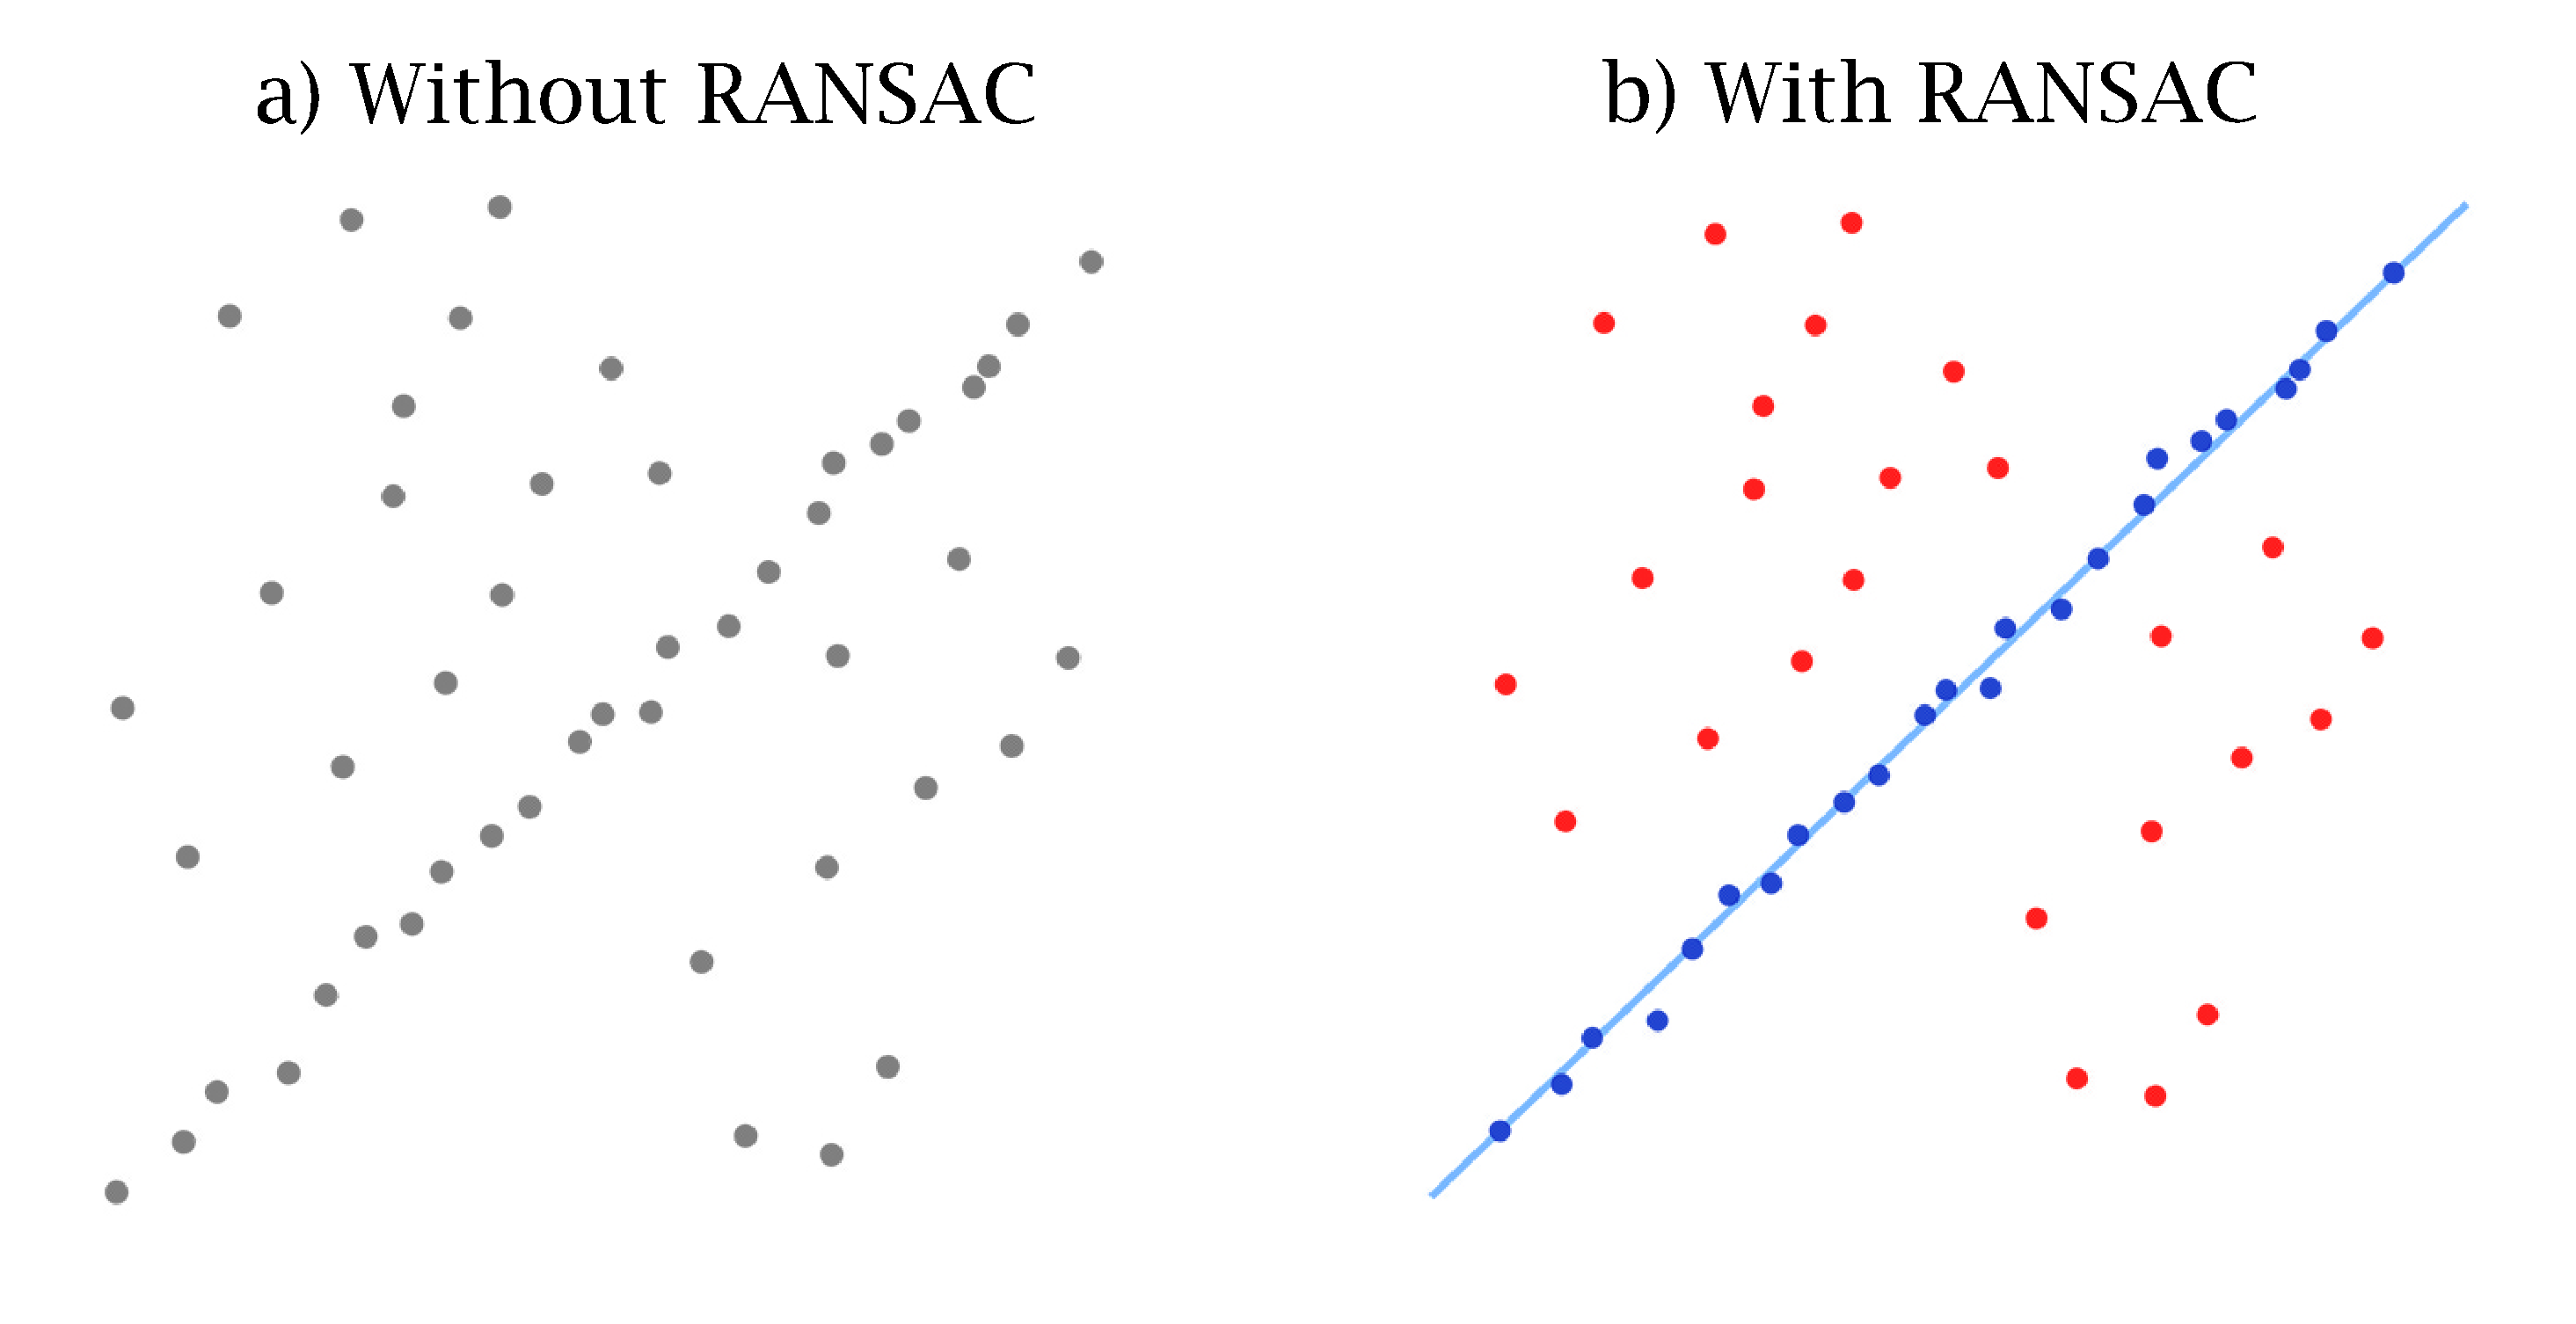
\includegraphics[width=0.8\linewidth]{figures/PDF/RANSAC.pdf}\\
        %\caption{Surroundness among connected components (b) and among borders (c)\cite{Suzuki}}
        \caption{ a) A data set without outliers and inliers distinguished\protect\footnotemark. b) The RANSAC algorithm applied to fit a line. Outliers in red are dismissed in the result\protect\footnotemark.}
        \label{fig:ransac chart}
    \end{minipage}
\end{figure}
\footnotetext[1]{\url{https://commons.wikimedia.org/wiki/File:Line_with_outliers.svg}}
\footnotetext{\url{https://commons.wikimedia.org/wiki/File:Fitted_line.svg}.}


\noindent By using RANSAC, a random subset, entirely consisting of inliers, would define the fitted line. Since the algorithm is based on the probability that a particular group of inliers should represent the fitted line, the accuracy of RANSAC is typically improved by more iterations. Except when overfitting the model, which can cause the algorithm to find a local minimum, giving poor results.


\subsubsection{Hough Transform}
The Hough Transform\cite{Duda} is a technique used to isolate simple shapes within an image. Initially, Hough Transform was created with the intent to find lines but has later been extended to identify positions of arbitrary shapes, most commonly circles and ellipses. By using a voting procedure, the purpose of Hough Transform is to identify imperfect instances of objects inside a certain class. Moreover, a simple shape is defined as one that can be represented by only a few parameters. For example, a line can be defined with two parameters: slope and intercept. A circle can be defined with three parameters: the coordinates of the center (x,y) and the radius (r).  \\

\noindent The standard Hough Transform is used for detecting lines and achieves this by describing a line in the Hesse normal form: \begin{equation} p = xcos(\theta) + ysin(\theta) \end{equation}  where $p$ is the perpendicular distance, in pixels, from the origin to the line, and $\theta$ represents the angle measured in radians, which is the orientation of $p$ as shown in \textit{Figure \ref{fig:hough graph} a)}. \\

\noindent Each line can now be represented in the ($p$, $\theta$) form, which implies that any value ($p$, $\theta$) corresponds to a line in two-dimensional parameter space. Therefore, every ($x$, $y$) value in an image can now be represented as a curve, according to \textit{Equation 2.2}. Furthermore, one can imagine this ($p$, $\theta$)-plane as the hough-space where every ($x$, $y$) value in an image are accumulated into this space. The result consists of several sinusoidal curves that cross where lines occur, as shown in \textit{Figure \ref{fig:hough graph}  b)}. Moreover, a voting procedure is used to tell where lines are in an image. For every point on a line, the corresponding accumulator cell is increased. Thereafter, finding the cells with the most peaks in the accumulator array tells where the lines are in the corresponding image. To better find the peaks in the accumulator array Hough Transform can use Morphological operations, like applying a threshold. However, different operations might yield different results depending on the image. Explanations of different morphological operations can be found in \textit{Section 2.3.2}

\begin{figure}[H]
    \centering
     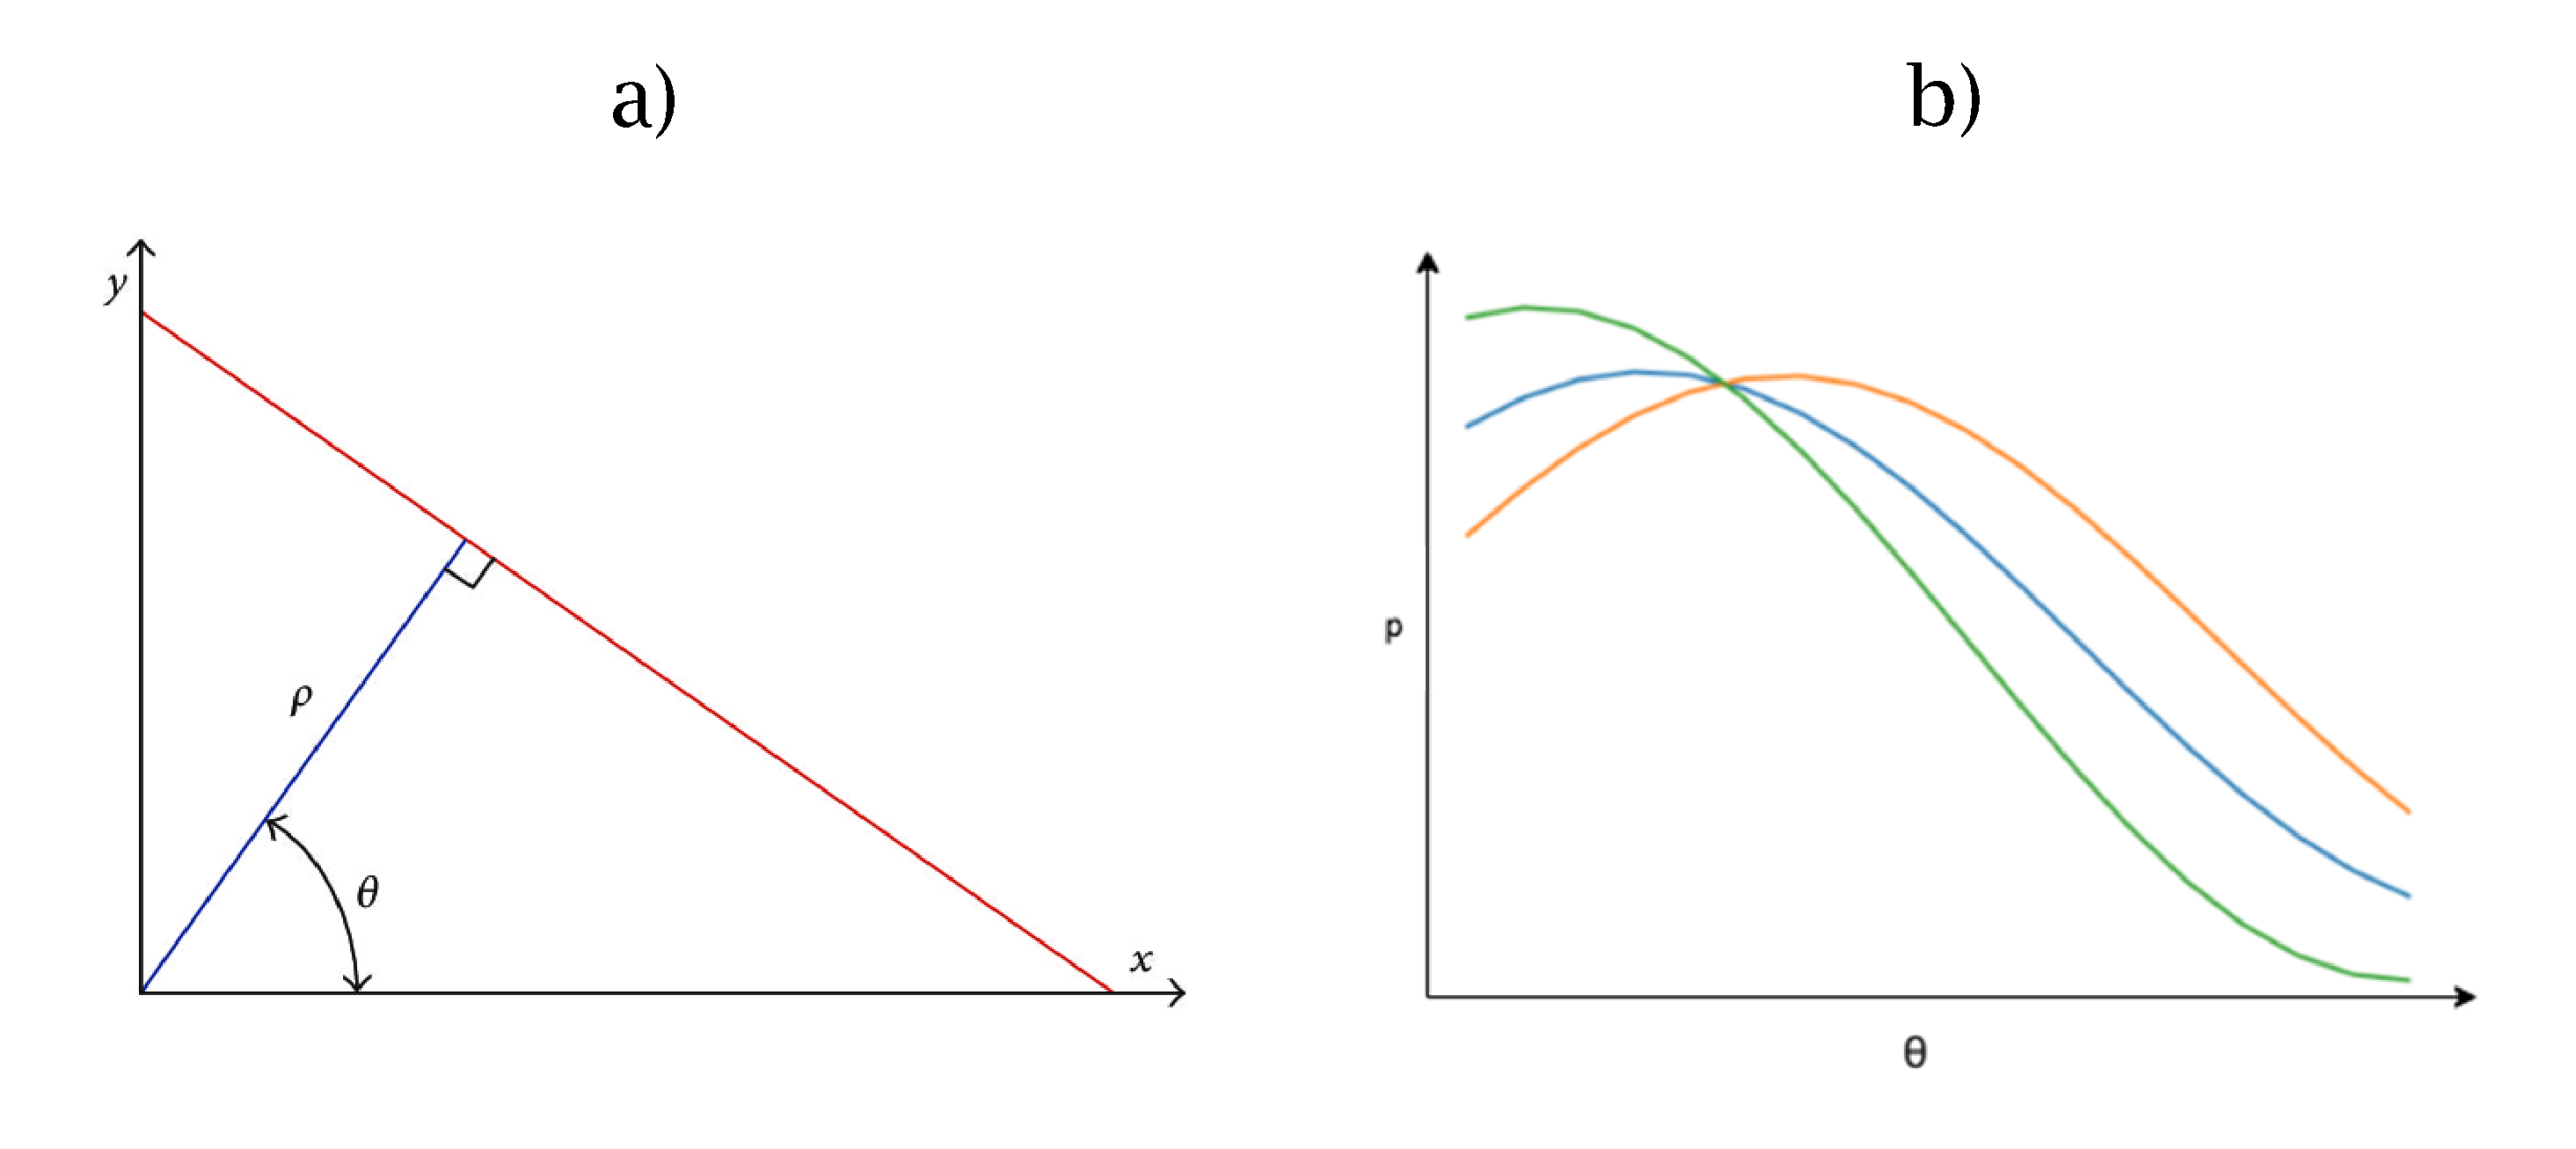
\includegraphics[width=1\linewidth]{figures/PDF/Hough_graph.pdf}\\
    \caption{a) Rho and theta parameters of a straight line\cite{Duda}. b) Three different colored curves obtained by \textit{Equation 2.2}. The intersecting point indicates a line with the parameters $p$ and $\theta$.}
    \label{fig:hough graph}
\end{figure}

\subsubsection{Modified Hough Transform}
Using modified versions of Hough Transform enables the technique to find shapes like circles and ellipses. To find circles in imperfect images, one can use Circle Hough Transform (CHT). The technique is similar to the standard Hough Transform, with the difference being that the parameter space is different. Therefore, the same procedure can be used in CHT to detect other features with other analytical descriptions. In general,  a circle can be described by: \begin{equation} {(x-a)}^2 + {(y-b)}^2 = r \end{equation} where ($r$) is the radius and ($a$, $b$) is the center of a circle. Forthwith, for every fixed ($x$, $y$) value in an image, every parameter in \textit{Equation 2.3} can be found. Therefore, the hough-space is now the ($a$, $b$, $r$)-plane. However, because the ($a$, $b$, $r$)-plane defines a three-dimensional space, the parameters can be identified in two stages. The first stage is to fix the radius to find the optimal center point in the two-dimensional parameter space. After that, the optimal radius can be derived in one-dimensional parameter space. Moreover, the computational complexity of the algorithm increases, the more parameters that exist in the parameter space. \\

%With image pre-processed with Canny, Hough Transform is used to isolate simple shapes within the image. The algorithm is divided into different parts, depending on what shape is of interest. To find the exact position of, e.g., a circular object, Circle Hough Transform looks for circular shapes using an accumulator matrix, which divides the images into groups of pixels (usually size 3x3). Following edges found using Canny, non-circular edges are ignored. Valid circular shapes are specified using parameters deciding radius interval, as well as the desired number of circles. The intersection point of the circle is later calculated, finding the center of the circle. Lastly defined and valid shapes in the image are identified and painted as seen in Figure 2. \\

%\noindent\begin{minipage}{.6\textwidth}
%  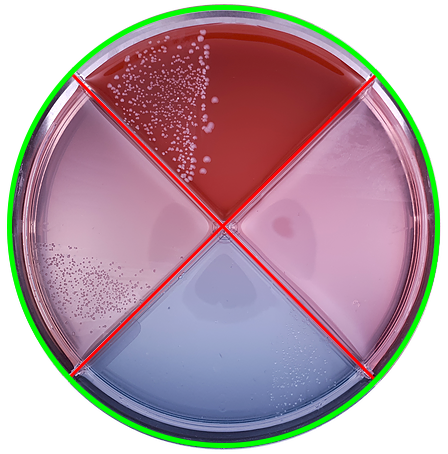
\includegraphics[width=.5\linewidth]{figures/hough.png}\\\\
%  \captionof{Fig. 2. }{Hough transformation is used to identify distinct shapes in images such as circles and lines.}
%  \label{fig:fig1}
%\end{minipage}



\subsection{Masking}
\noindent Region-of-interest (ROI) processing is an approach aiming to extract that information from a specific subregion of an image. The ROI is usually defined by points, lines, circles, or other shapes, which is then used to apply a binary mask to the image. The binary mask is created with the same size as the input image. Pixels within the ROI is set to 1 and the remaining pixels to 0. \textit{Figure \ref{fig:masking}} illustrates before and after masking, where the ROI is the agar plate. \\ 

\begin{figure}[H]
    \centering
    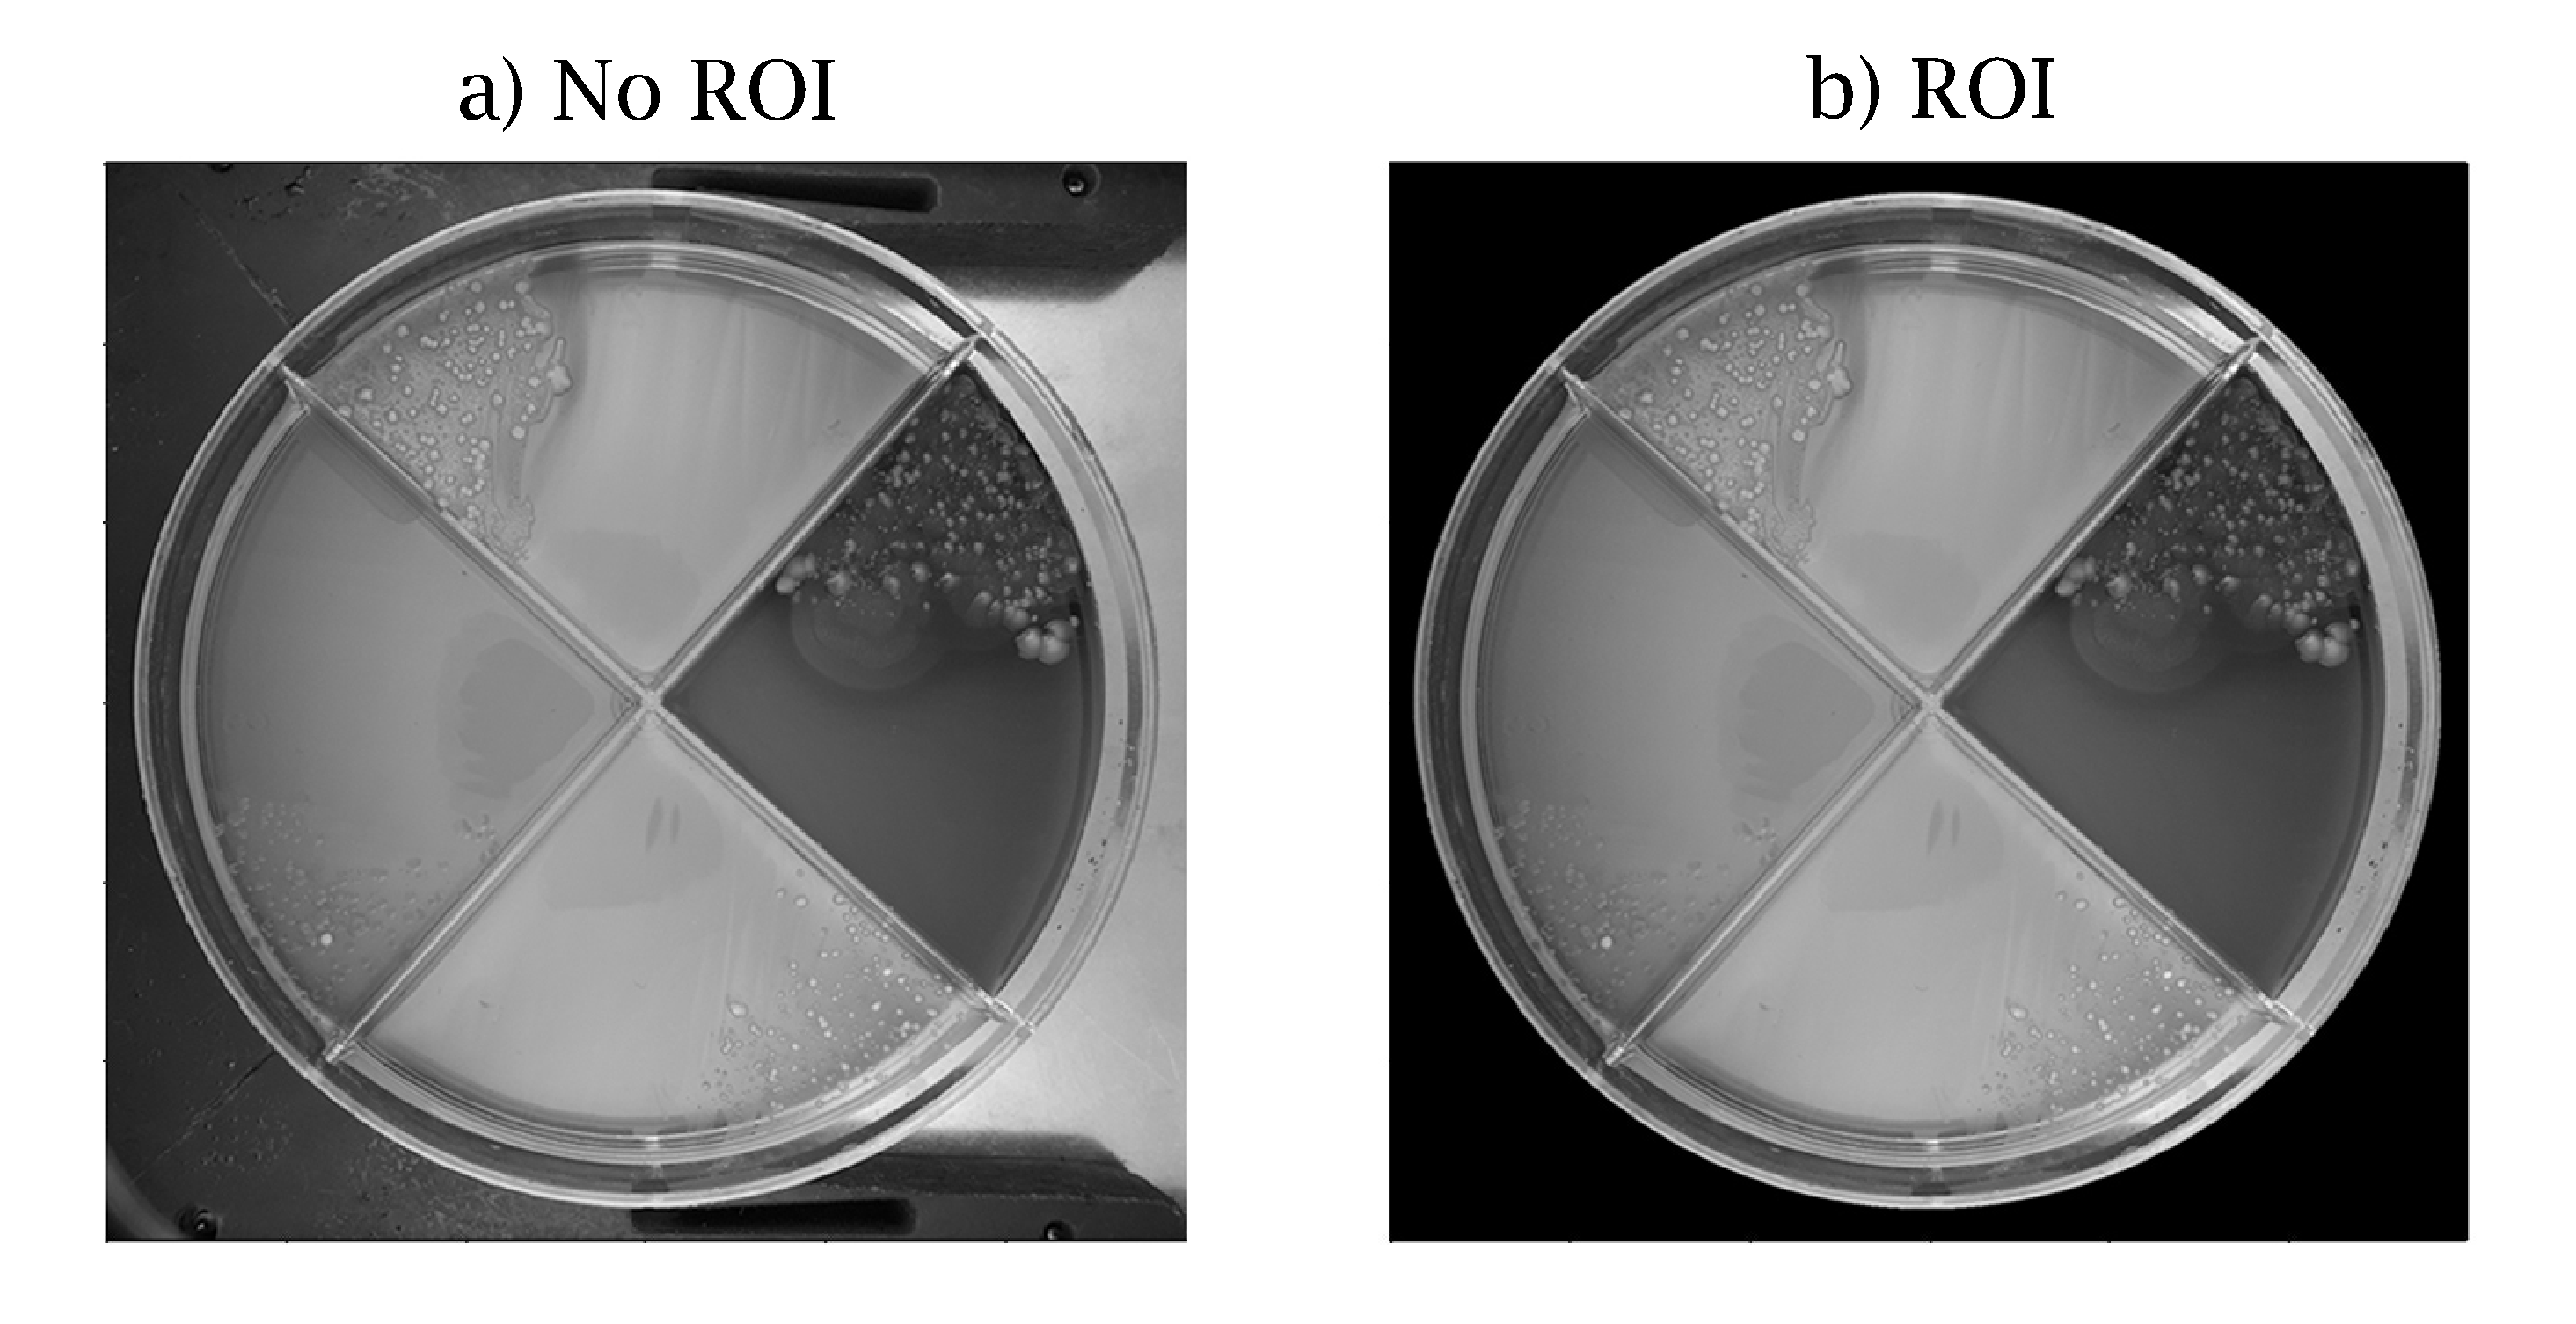
\includegraphics[width=0.8\linewidth]{figures/PDF/ROI.pdf}\\
    \caption{Figure illustrates an image with and without masking of irrelevant data using points given by \texit{Circle Hough Transform}}
    \label{fig:masking}
\end{figure}

\subsection{Color Space Image segmentation}
In circular shaped objects, it can sometimes be challenging to determine the rotation. With the human eye, one can recognize a specific shape, color, or feature within an object that only occurs in a particular direction, thus determine the rotation. This rotational landmark can be extracted using \textit{Image Segmentation}\cite{Rahmat}, which simply divides groups of pixels together based on given criteria.\\  


\noindent In \textit{Figure \ref{fig:segmentation} a)}, a compartment in distinctive red can be distinguished in the right half of the image. In order to extract the orientation data of this compartment, its pixels need to be segmented. To segment areas based on color, criteria can be defined by Color Spaces, which are colors represented of their different components, e.g., RGB (Red, Green, Blue) or HSV (Hue, Saturation, Value). For example, in \texit{Figure \ref{fig:segmentation} b), the red tones in the HSV-space are, in this case, generally more localized and visually separable. The RGB-space in \texit{Figure \ref{fig:segmentation} c)}, on the other hand, shows that the red tones have a larger span across both the green and blue axis.}
By adjusting color space values, different information can be extracted from the image. For example, changing the Red in RGB to 0 would remove all red tones in a picture, leaving only a spectrum of green and blue.\\

\begin{figure}[H]
    \centering
     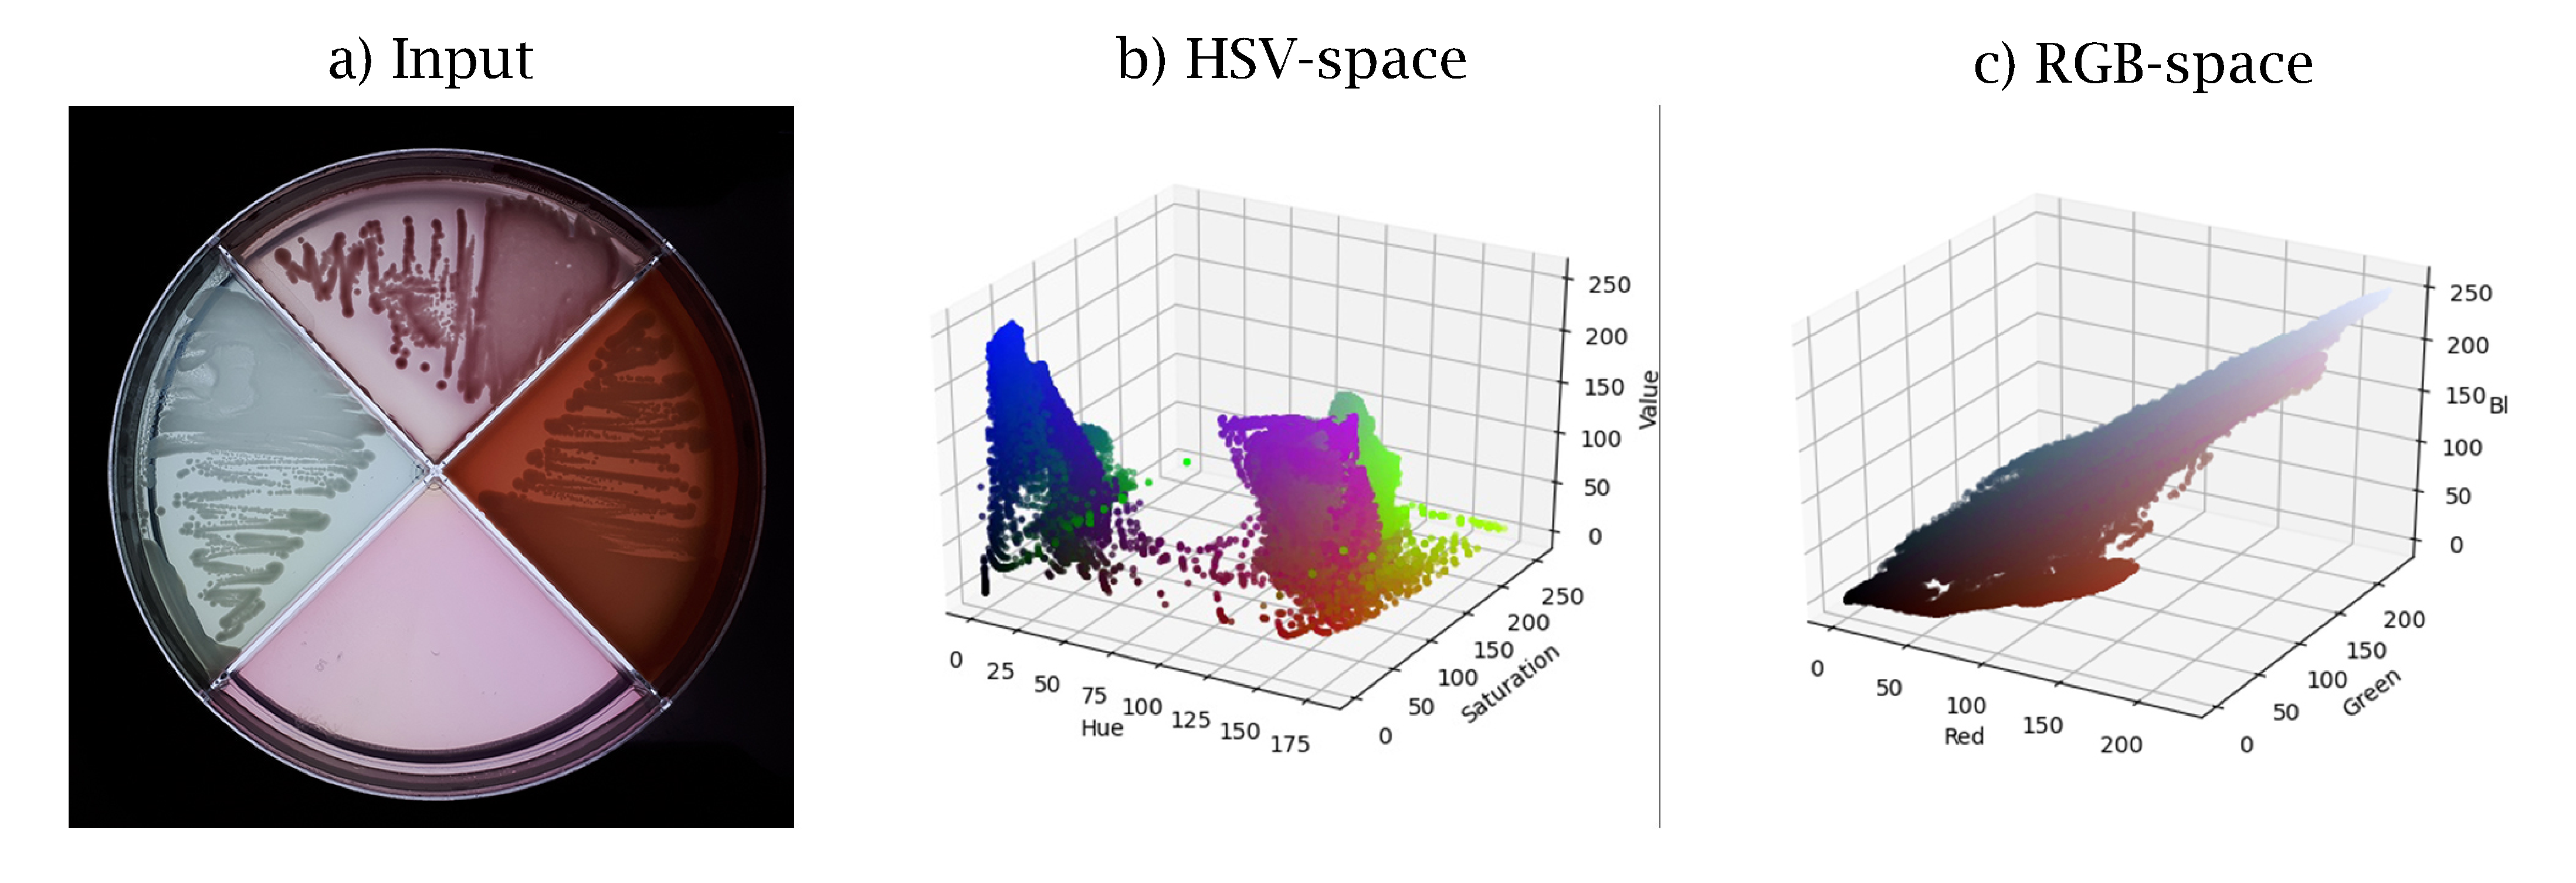
\includegraphics[width=1.1\linewidth]{figures/PDF/Color_space.pdf}\\
    \caption{{a) Example of an input image with a distinctive red-colored compartment. b) An HSV-space 3D scatter plot of the input. c) An RGB-space 3D scatter plot of the input.}}
    \label{fig:segmentation}
\end{figure}


\subsection{Image registration}
Misalignment in images is a common issue and can happen for a variety of reasons. However, the most common is due to images being captured under variable conditions, such as changes in camera perspective or the scene content. Image registration\cite{Nag} is a technique used in medical sciences, remote sensing, and computer vision that corrects misaligned images. The fundamental idea is to align two or more images of the same scene with one image designated as the reference image. Thus, getting an image matching the reference image (see \textit{Figure \ref{fig:image reg}}). There exist multiple image registration techniques, but the majority of them can be broken down into the following steps described below: \\
\begin{enumerate}
    \item \textit{Feature detection:} The detection process of different features in an image. This process can be manual or automatic; however, automatic detection is preferable. Moreover, an example of features this process looks for is edges, contours, closed-boundary regions, line intersections, and corners. Different image registration techniques can be divided into intensity-based or feature-based. Briefly, intensity-based methods look for distinctive edges in an image whereas, feature-based looks for specific objects which are more prevalent in computer vision. 
    \item \textit{Feature matching:} The process of matching the different features detected in the reference image and those detected in the non-aligned pictures (sensed images). 
    \item \textit{Transform model assessment:} The parameters of the mapping functions are estimated by aligning the sensed image with the reference image. 
    \item \textit{Image transformation:} The sensed image is transformed by employing the mapping functions.
\end{enumerate} 
\ \\
\noindent The tasks described above have typical problems, and problems might occur if specific requirements are not obtained\cite{Zitova}. The detection of features should be distinctive objects or objects spread over the image, which are easily detectable. Moreover, the feature matching between the sensed image and the reference image needs to have enough common features to achieve proper registration. Especially, on occasions when the images do not cover the same scene, object collision occurs or other unexpected changes. \\

\begin{figure}[H]
    \centering
     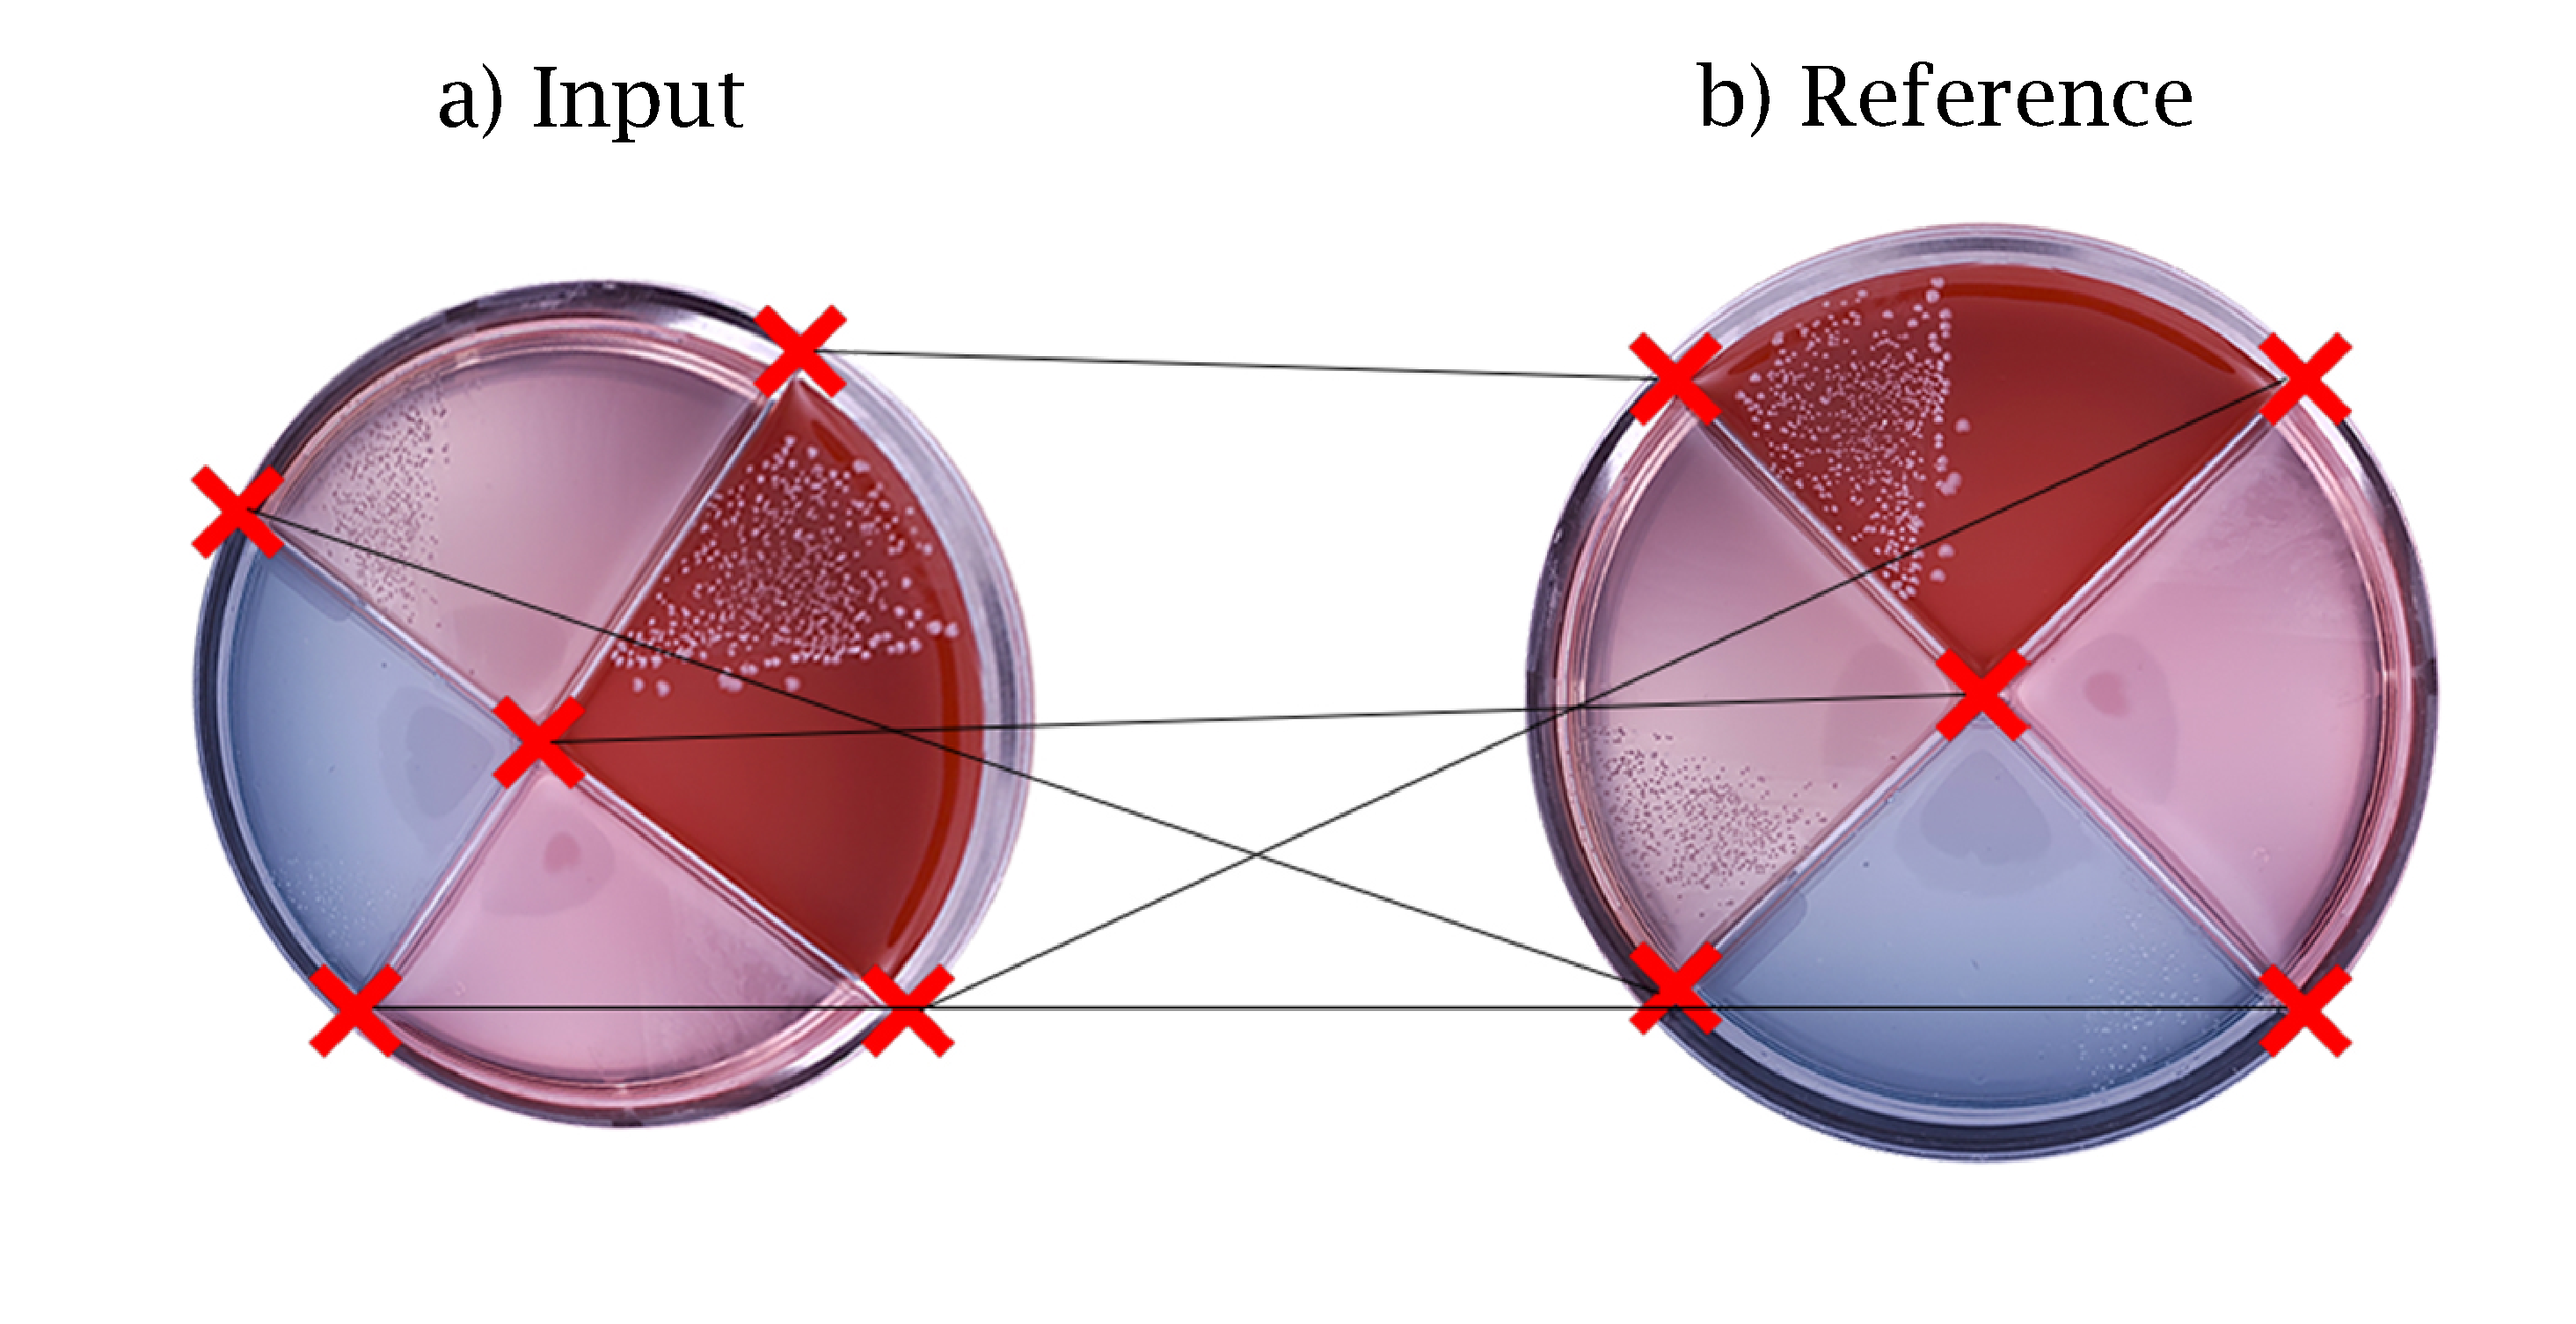
\includegraphics[width=0.8\linewidth]{figures/PDF/Image_reg_theory.pdf}\\\\
    \caption{a) Will be adjusted to mimic the reference image in b) as close as possible, based on the reference points}
    \label{fig:image reg}
\end{figure}

\subsubsection{Different transformation models}
Different image registration techniques\cite{Nag} can also be classified depending on what transformation models they use. The most used are linear transformations followed by projective transformations. However, there also exist non-linear transformations, but it is beyond the scope of this work. Linear transformations include transformation on rotation, translation, scaling, and shearing in images, and are collectively known as affine transforms. The transformation in a two-dimensional space is done by determining the transformation matrixes shown below: \\

\noindent\begin{enumerate}
    \item \textit{Rotation:}  object can be rotated given an angle $\theta$ proportionate to its origin.  \begin{equation} \begin{bmatrix} x_{1} \\ y_{1} \end{bmatrix} = \begin{bmatrix} cos\theta & sin\theta \\ -sin\theta & cos\theta \end{bmatrix} + \begin{bmatrix} x_{2} \\ y_{2} \end{bmatrix} \end{equation} $(x1, y1)$ is the new point, $(x2, y2$) is the old point, and $\theta$ is the rotation parameter. \\
    \item \textit{Scaling:} Scaling is done to resize an image or to match images with different sizes.  \begin{equation} \begin{bmatrix} x_{1} \\ y_{1} \end{bmatrix} = \begin{bmatrix} s_{x} & 0 \\ s_{y} & 0 \end{bmatrix} + \begin{bmatrix} x_{2} \\ y_{2} \end{bmatrix} \end{equation} Where $(x1, y1)$ is the new point, $(x2, y2)$ is the old point, and $(s1, s2)$ is the scaling parameters. For example, if $s1 = 2$ and $s2 = 2$ the old point $(x2, y2)$ is scaled by two in every direction. \\
    \item \textit{Translation:} If a point x,y  is to be translated by t units then, the transformation matrix is: \begin{equation} \begin{bmatrix} x_{1} \\ y_{1} \end{bmatrix} = \begin{bmatrix} x_{2} \\ y_{2} \end{bmatrix} + \begin{bmatrix} t_{1} \\ t_{2} \end{bmatrix} \end{equation} where $(x1, y2)$ is the new point, $(y2, x2)$ is the old point, and $(t1, t2)$ is the translation value. \\
    \item \textit{Shearing:} Shearing slants the shape of an object. There exist two sheering transformations, x-shear, which changes the values of the coordinates and y-shear, which changes the values of the y coordinates.  \begin{equation} \begin{bmatrix} x_{1} \\ y_{1} \end{bmatrix} = \begin{bmatrix} a_{11} & a_{12} \\ a_{21} & a_{22} \end{bmatrix} \begin{bmatrix} x_{2} \\ y_{2} \end{bmatrix} + \begin{bmatrix} a_{13} \\ a_{23} \end{bmatrix}  \end{equation} where $(x1, y2)$ is the new point, $(x2, y2)$ is the old point, and $(a_{11}, a_{12}, a_{21}, a_{22}, a{13}, a{23}$ is the sheering parameters.  \\
    \item \texit{Reflection:} Reflection is done by mirroring an image of the original object. Simply, reflection does not change the size of the object. 
\end{enumerate}
\ \\
\noindent The difference between linear transformations and projective transformations is that linear transformations are global by nature. Therefore, the geometrical difference between images cannot be modeled. However, projective transformations allow for warping a target image to match a reference image, which is achieved by a homography. A homography is a transformation matrix that maps points from the target image to the corresponding point in the reference image as follows:  \begin{equation} \begin{bmatrix} x_{1} \\ y_{1} \\ 1 \end{bmatrix} = H \begin{bmatrix} x_{2} \\ y_{2} \\ 1 \end{bmatrix} =  \begin{bmatrix} h_{00} & h_{01} & h_{02} \\ h_{10} & h_{11} & h_{12} \\ h_{20} & h_{21} & h_{22} \end{bmatrix} \begin{bmatrix} x_{2} \\ y_{2} \\ 1 \end{bmatrix} \end{equation} Where H is the homography matrix.  

\subsection{Image accuracy validation}
When working with large datasets, manual validation of each output may be too time-consuming and a waste of resources. By automating the validation process for each output, higher accuracy can be achieved as well as saving time otherwise spent on debugging.  \\

\noindent For shape oriented image processing, different types of \textit{Image moment}\cite{Huang}\cite{Chaumette} algorithms can be used. Image moments are values of the weighted average of pixel intensities in images, which can then be used to compare two images. The moment of a single-channel binary image, for example, is defined as \textit{Equation 2.9}, with I(x, y) being the intensity of a pixel on a given x,y coordinate. \begin{equation}
    M = \sum_x \sum_y{I(x, y)}
\end{equation} The formula can be extended to consider both pixel intensity, as well as its position in the image using \textit{Equation 2.10}. However, this method is not entirely transformational invariant.\\ \begin{equation}
    M_i_j = \sum_x \sum_y{x_iy_jI(x, y)}
\end{equation} 

\noindent As an extension to image moments, \textit{Central moments} can be used to address translation and scale-varieties. The central moment is defined using \textit{Equation 2.11}. Where $\overline{x}$ and $\overline{y}$ are the weighted averages of pixels constituting different shapes (or blobs) found in an image.\\

\begin{equation}
    \mu_i_j = \sum_x \sum_y{(x - \bar{x})^i(y - \bar{y})^jI(x, y)}
\end{equation}  
 
\noindent For the moments to be scale-invariant, the \textit{Normalized Central Moments} are calculated as follows in \textit{Equation 2.12.}\\
\begin{equation}
    \eta_i_j = \frac{\mu_i_j}{(i+j)/2+1}
\end{equation} 
 
\noindent Even though the normalized central moments are translation and scale-invariant, rotation is still something to take into consideration. An algorithm called Hu Moments addresses this problem using a set of 7 values. Each value is calculated using Normalized Central Moments, where the first six moments address translation, scale, rotation, and reflection, and the last moment is skew invariant, which can identify mirror images.





%%%%%%%%%%%%%%%%%%%%%%%%%%%%%%%%%%%%%%%%%%%%%%%%%%%%%%%%%%%%%%%%%%%%%%
%%% lorem.tex ends here

%%% Local Variables: 
%%% mode: latex
%%% TeX-master: "demothesis"
%%% End:

\chapter{Related Work}
\label{cha:related work}
This chapter addresses previous work in image processing that tries to solve similar problems this thesis does. There exist several methods on how to identify different shapes and varieties in angle, rotation, position, and scale in images. However, no study found solves a similar problem this thesis does. Therefore, this chapter focuses on related work using similar techniques written about in the theory chapter. 

\section{Edge detection}
Many recent papers have focused on Canny Edge Detection and similar techniques to detect edges in images. \cite{Genesan} did a study of different edge detection methods for various image processing applications. The same edge detection algorithm can not be applied for all types of images since edge detection methods are problem-oriented. Because it is challenging to perform edge detection in noisy images, the authors compare different edge detection methods with their advantages and limitations. Canny edge detection produced excellent results, especially under noisy conditions.\\

\noindent Moreover, many recent papers have focused on improving Canny Edge Detection to detect edges in noisy images better. \cite{Nikolic} proposes an improvement by using a modified median filter instead of Gaussian smoothing. The algorithm could successfully remove, with optimal threshold values on the canny operator, noise from an ultrasound image of a kidney. \cite{Rong} suggests an adaptive threshold selection method for the Canny Edge Detection algorithm to preserve more useful edges and more robust noise.

\section{Shape detection}
In work for pupil identification, \cite{Soltany} suggests using a combination of the two techniques Canny Edge Detection and Hough Transform to detect pupils in images. The canny operator is used to identify the edge of a pupil, while Hough Transform finds the exact position. The proposed algorithm managed to accurately fit circles of different eye images under different lighting conditions. Additionally, \cite{Divya} presents an algorithm that can detect and outline the outer edge of the pupils in human eyes using Hough Transform and Canny Edge detection. The algorithm was tested on 100 human eyes and produced a 95\%  successful result.\\

\noindent RANSAC is a popular method of choice for model fitting to find ellipses in images. \cite{Bozomitu} suggests an algorithm using the RANSAC procedure for pupil detection. Using RANSAC provides high accuracy with low running time in normal and noisy conditions and for variable illumination. \cite{Xie} proposes an ellipse detection method using RANSAC that achieves high accuracy and computation cost in detecting multiple ellipses in images. The algorithm works in two steps. Firstly, region segmentation and contour detection are applied. Secondly, with each contour segment found, a modified RANSAC is applied to five randomly selected pixels to form an accurate ellipse.

\section{Image Registration}
There are numerous image registration methods, which are frequently used in medical imaging, automatic target recognition, and computer vision. \cite{Saxena} provides knowledge of different image registration methods and their use in various application areas by discussing their advantages and disadvantages. The techniques are divided into two groups, Area-based and feature-based. Feature-based techniques find correspondence in salient features in images such as lines, points, and contours. Area-based methods, however, emphasize on feature matching without the detection of salient objects.  \\
%section{Morphological identification}

%\section{Managing different shapes and perspectives in images}

%%% lorem.tex --- 
%% 
%% Filename: lorem.tex
%% Description: 
%% Author: Ola Leifler
%% Maintainer: 
%% Created: Wed Nov 10 09:59:23 2010 (CET)
%% Version: $Id$
%% Version: 
%% Last-Updated: Wed Nov 10 09:59:47 2010 (CET)
%%           By: Ola Leifler
%%     Update #: 2
%% URL: 
%% Keywords: 
%% Compatibility: 
%% 
%%%%%%%%%%%%%%%%%%%%%%%%%%%%%%%%%%%%%%%%%%%%%%%%%%%%%%%%%%%%%%%%%%%%%%
%% 
%%% Commentary: 
%% 
%% 
%% 
%%%%%%%%%%%%%%%%%%%%%%%%%%%%%%%%%%%%%%%%%%%%%%%%%%%%%%%%%%%%%%%%%%%%%%
%% 
%%% Change log:
%% 
%% 
%% RCS $Log$
%%%%%%%%%%%%%%%%%%%%%%%%%%%%%%%%%%%%%%%%%%%%%%%%%%%%%%%%%%%%%%%%%%%%%%
%% 
%%% Code:


\chapter{Method}
This chapter will summarize and describe the methods and approaches used to answer the problems stated in \textit{Section 1.3}. The first section will describe the workflow proposed to generate the final results. The second section describes how the results will be evaluated.

\section{Implementation}
\noindent The work will be implemented in steps described in \textit{Figure \ref{fig:method workflow}}. Each step is dependent on the output of its predecessor. The first step is to identify and mask the agar plate. With the irrelevant data masked, the second step is to identify the compartment edges in the agar plate. With the agar plate and its compartment edges identified, the orientation will be calculated based on the output of the previous steps. Lastly, based on gathered key points, the images will be processed using image registration. \\

\begin{figure}[H]
    \centering
     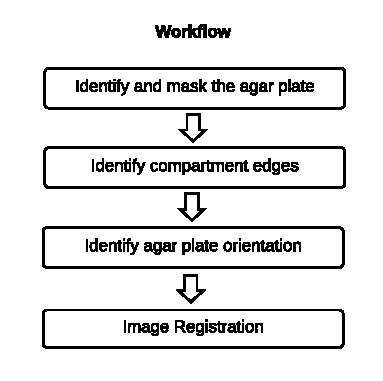
\includegraphics[width=.43\linewidth]{figures/PDF/Workflow.pdf}\\
    \caption{Workflow of the implementation structure}
    \label{fig:method workflow}
\end{figure}

\subsection{Identify and mask the agar plate}
The first step is to identify the agar plate, which will provide an elliptical contour of points that defines the ROI. The workflow will be structured, as shown in \textit{Figure \ref{fig:identify and mask flowchart}}, and described throughout the section. 
\begin{figure}[H]
    \centering
    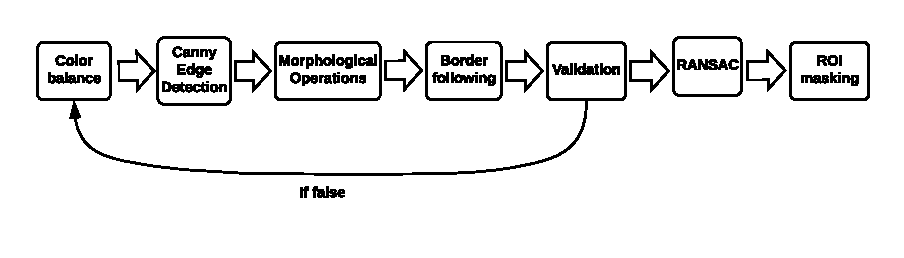
\includegraphics[width=1\linewidth]{figures/PDF/Identify and mask agar plate.pdf}\\
    \caption{Flowchart to identify and mask the agar plate.}
    \label{fig:identify and mask flowchart}
\end{figure}

%\noindent \textbf{Color balance} \\
%\noindent \color{red} Describe the brightness and contrast algorithm in the Theory section. \color{black} 

\noindent Different images might not have the same conditions regarding the illumination or intensity of RGB values, which means that each image might not get the same result when being processed.  Therefore, it is essential to even out these variables. However, images that are too dark or too bright may not take full advantage of color balancing; they may also need to balance brightness and intensity beforehand.  Each input will, therefore, be processed in terms of balancing brightness and contrast, followed by color balancing using SCB before further processing. The goal of this step is to improve the accuracy of the final output. \\

%\noindent\textbf{Canny, Thresh, Morph}\\
\noindent With contrast, brightness, and color all balanced, the next step is to process the image using Canny to intensify edges and reducing any image noise. Before applying Canny, an additional Gaussian blur will firstly be applied to reduce any bacteria within each compartment. Configuring Canny to the desired level with a minimal number of bacteria clusters, however, might cause disconnectivity in the outer contour. Morphological operations such as Closing will then be used to repair any broken lines. \\ 


\noindent The next step is to define any contours. CHT could be used to identify a perfectly circular contour, but due to variations in perspective, the agar plate will always be a bit elliptical. Using CHT, in this case, would give inaccurate results. Therefore, the contour will be found using border following. The contour found in the highest hierarchy should represent the external contour of the agar plate. However, some segments of the contour may, in some cases,  be imperfect due to, e.g., bacteria clusters growing close to the edge. The contour will, therefore, be fitted to an elliptical model using RANSAC, which should give a better approximation of the external contour, providing the desired set of key-points.  
%\\\color{red} “Mention in the Theory chapter that contours a sorted in hierarchies.” \color{black}  \\


\noindent Each image will be validated before proceeding to the final step of this section. The contour defined with conic fitting will then be compared with an approximated contour found using CHT. The comparison will be made using Hu Moments. Since the conic fitting contour will be elliptical and the contour from CHT always will be circular, a margin of error will be considered. If the Hu Moment returns a value exceeding the margin of error, the whole workflow process will be repeated. Invalid matches may be the result of bacteria clusters covering segments of the agar plate edges in shadowed areas. However, the problem can be solved by increasing or decreasing the initial brightness or contrast. The image will be reprocessed until a valid match is found. \\  

\noindent Lastly, with the ROI defined by the contour key-points from previous steps, a binary mask will be applied to the image, removing the unwanted background.\\


\subsection{Identify compartment edges}
\noindent The second process is to identify the compartment edges and the center point on the agar plate. Each compartment divider can be segmented as two straight lines i.e., compartment edges. Therefore, by using Hough Transform, these shapes can be identified. However, some pre-processing is needed to identify the edges correctly and reduce irrelevant noise that might occur. \textit{Figure \ref{fig:compartment edges flowchart} } illustrates how the workflow is structured. \\


\begin{figure}[H]
    \centering
     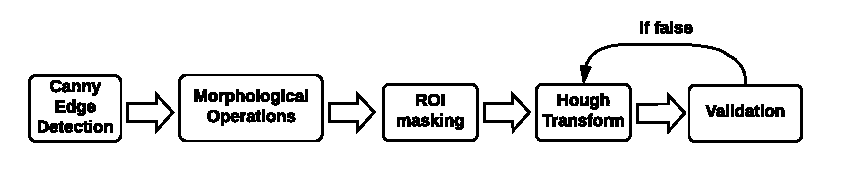
\includegraphics[width=0.9\linewidth]{figures/PDF/Identify compartment edges.pdf}\\
    \caption{Workflow to identify the compartment edges and the center point of the agar plate.}
    \label{fig:compartment edges flowchart}
\end{figure}

\noindent Once again, Canny, with an extra Gaussian blur, is applied to identify only the most distinct edges. The difference in this case, compared to finding the outer contour, is that only the centermost line of the compartment edges is of interest. As seen in \textit{Figure \ref{fig:compartment masking} b)}, each compartment divider consists of two edges, one on each side. Finding the centermost line is important since the intersection between the two crossing compartment edges constitutes the actual center point of the agar plate. The edges of each side of each compartment division can be merged to form one thick line using Morphological Closing. By using Skeletonize, the line can then be reduced to represent a pixel-wide centerline of each divider. \\

\noindent The mask boundaries from the previous section will be reused. The mask will be reduced in size, leaving a new ROI. As shown in \textit{Figure \ref{fig:compartment masking} a)}, the area outside the drawn boundary is not needed to identify the positioning and angle of the compartment edges, and should, therefore, be masked. \\


\begin{figure}[H]
    \centering
    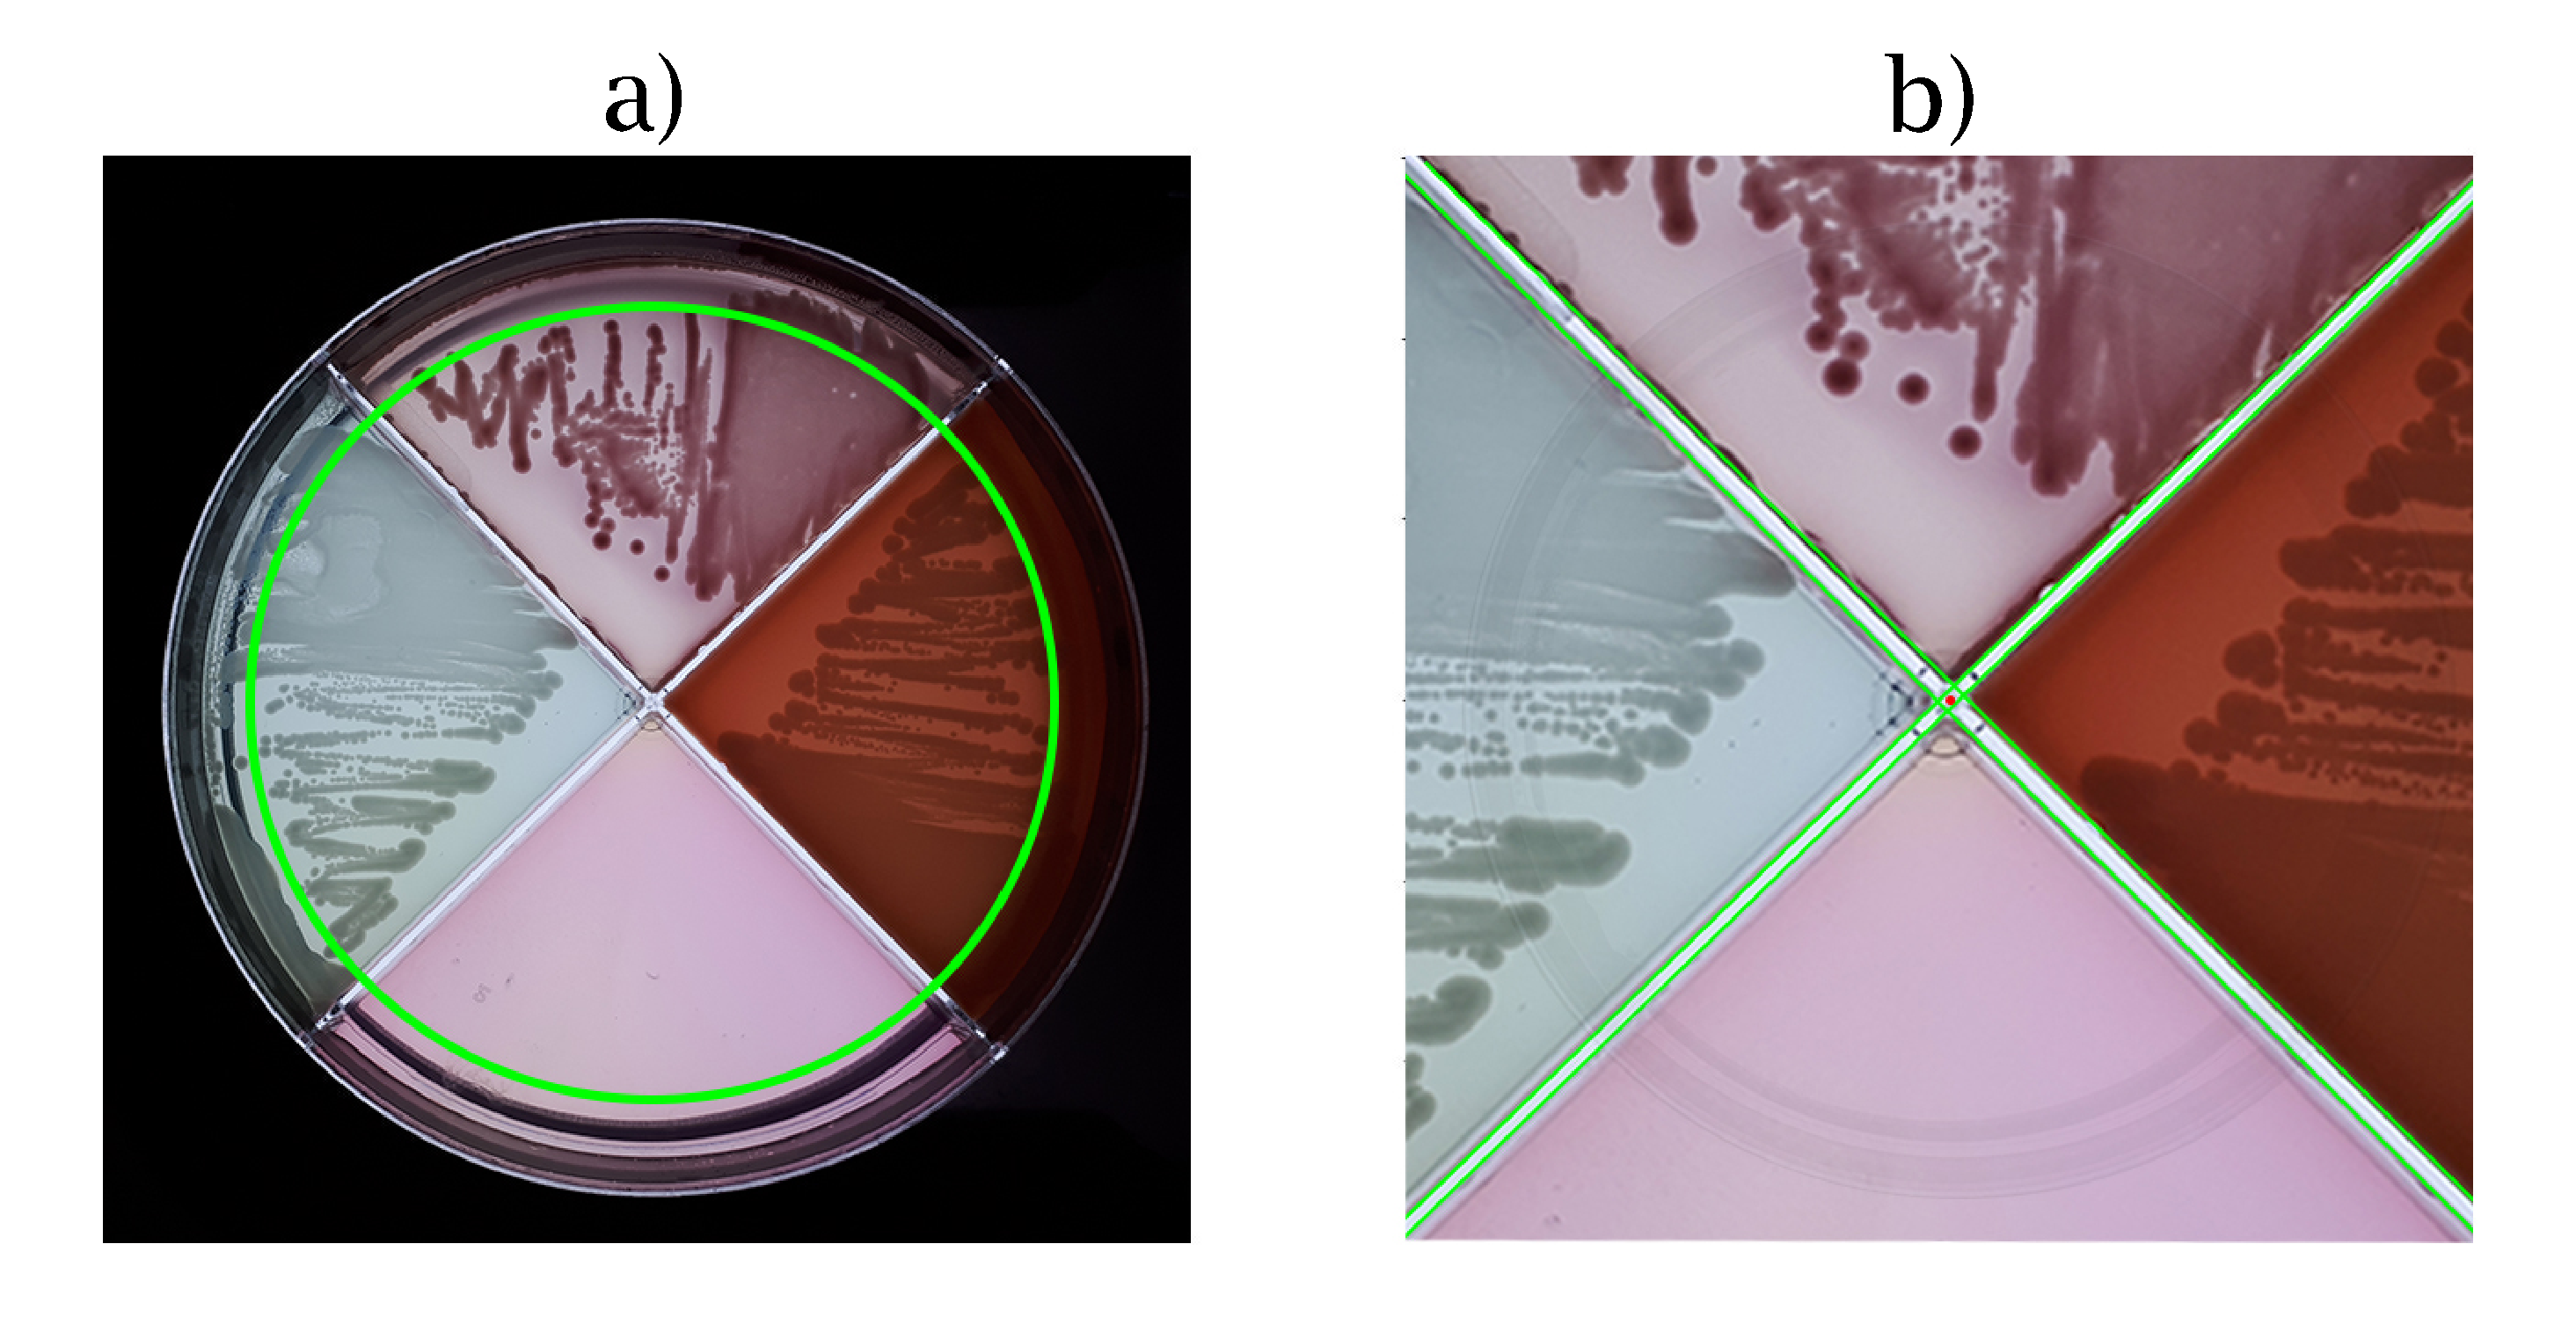
\includegraphics[width=.8\linewidth]{figures/PDF/ROI_boundaries.pdf} \\
    \caption{a) illustrates the new ROI boundary. b) show the edges and intersection (i.e., center point) of the compartment edges.}
    \label{fig:compartment masking}
\end{figure}

\noindent With a binary image representing the skeleton of the compartment edges, Hough Transform is used to identify the skeleton as lines. Lines will be sorted and validated in pairs based on values of rho and theta to make sure that only one line in each direction of the dividers is found. \\

\subsection{Identify agar plate orientation}
This part will focus on how to detect the rotation of the agar plate using segmentation. As shown in \textit{Figure \ref{fig:orientation flowchart}}, color space segmentation will be used to define the agar plate orientation, and key-points extracted from the previous sections can lastly be sorted considering rotation.\\ 
 
 \begin{figure}[H]
     \centering
      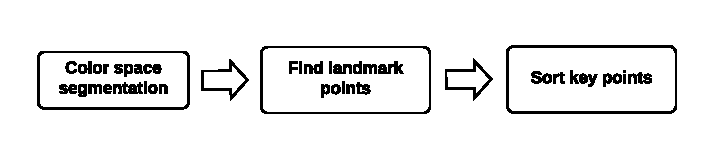
\includegraphics[width=0.7\linewidth]{figures/PDF/Identify agar plate orientation.pdf}\\
     \caption{Flow chart to identify the orientation of the agar plate.}
     \label{fig:orientation flowchart}
 \end{figure}


\noindent In the image dataset, the red compartment found in each image stands out. Since any compartments within an agar plate typically need to be distinguishable to the human eye,  color-based landmarks could be generally assumed here. The location of the segmented compartment will then be used to calculate the orientation.\\

\noindent Selecting the most prominent color should result in the most accurate output. The first step is to analyze both the HSV- and RGB-space of the image, generating corresponding 3D scatter plots of their color space. The color space providing the most visually separable and localized tones of red should be chosen. From the color space chosen, values from the scatter plot can be read to apply approximated values to the image.\\

\noindent With the selected compartment segmented, the intersection points between the outer contour in \textit{Section 4.1.1} and the lines from \textit{Section 4.1.2} are calculated as a first step to find the landmark points. Pixels on a line between each intersection point will be checked clockwise, forming a rectangular bounding box. A mean value of the pixel intensity on each line will be calculated. The line with the highest mean value should be the one crossing the segmented compartment, and the start- and end coordinate of the line will then define the first two landmark points. Remaining two intersection points will then be sorted clockwise in ascending order. From the sorted intersection point, all key-points from the previous two sections will lastly be sorted considering the rotation.


\subsection{Image registration}
The final touch is to transform the input image to match a reference using image registration. Since each input image will be different, key points from the previous sections will be sorted automatically and matched to a reference. The reference will be defined by key points representing, in this case, a completely symmetrical agar plate structure, as shown in \textit{Figure \ref{fig:keypoint structure}}.  Based on the sorted landmark points from \textit{Section 4.1.3}, all key points gathered so far will be sorted considering the rotation.\\

\begin{figure}[H]
    \centering
    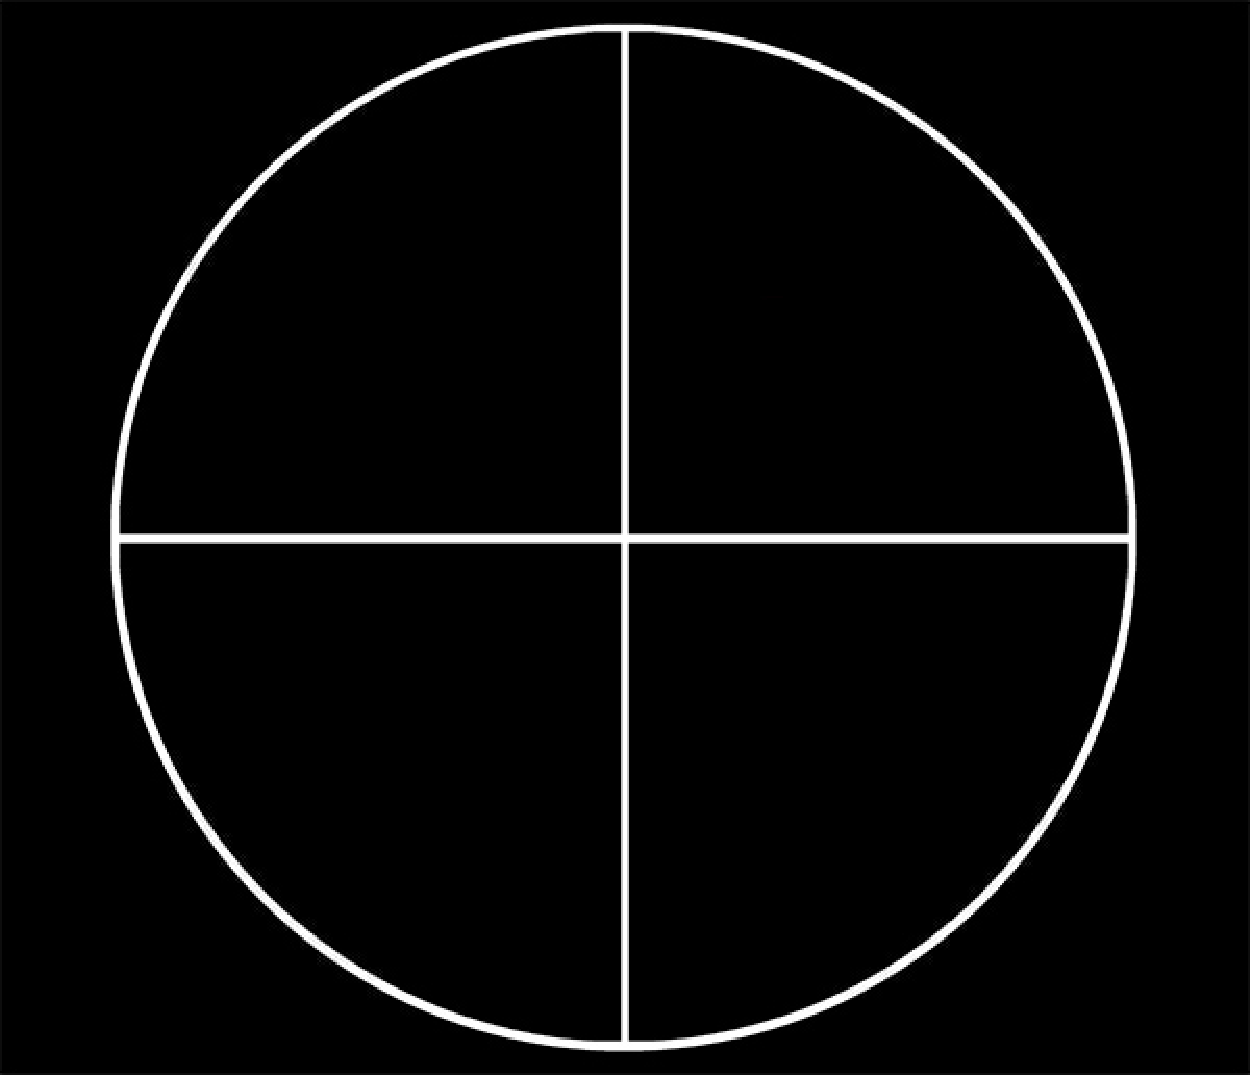
\includegraphics[width=0.3\linewidth]{figures/PDF/Ref_structure.pdf}\\
    \caption{Illustration of a structure based on pre-defined reference key points.}
    \label{fig:keypoint structure}
\end{figure}

\noindent With the key points and its corresponding matches, the homography can now be calculated to finally warp the image to the pre-defined reference points, thus completing the image registration.\\

\noindent Lastly, the elliptical projection of the agar plate, as illustrated in \textit{Figure \ref{fig:method projection}}, needs to be considered to improve the perspective accuracy in the more extreme cases. Since the goal is to produce a flat projection of the agar plate, additional iterations of the whole process will be applied to cope with any perspective distortion.

\begin{figure}[H]
    \centering
    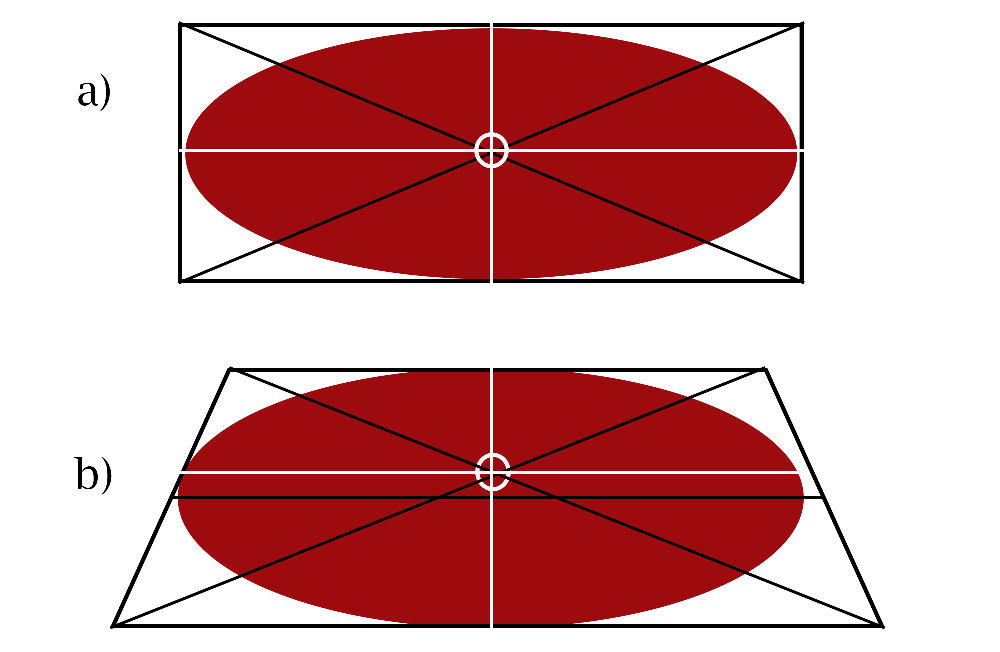
\includegraphics[width=0.5\linewidth]{figures/PDF/Ellipse_projection.pdf}\\
    \caption{a) Flat ellipse. b) Foreshortened circle (spatial illusion).}
    \label{fig:method projection}
\end{figure}

%\color{red} Should we write matches or descriptors? What is the difference? \color{black}


\section{Evaluation}
The approach of this thesis is to evaluate if a combination of image processing techniques can be used to solve the problem description. The thesis problem is assumed to be solved if the criteria in \textit{Section 1.3} are fulfilled. Therefore, the basis of evaluation for this method is to examine if the workflow, shown in \textit{Figure \ref{fig:method workflow}}, can produce results that fulfill the criteria. 


%%%%%%%%%%%%%%%%%%%%%%%%%%%%%%%%%%%%%%%%%%%%%%%%%%%%%%%%%%%%%%%%%%%%%%
%%% lorem.tex ends here

%%% Local Variables: 
%%% mode: latex
%%% TeX-master: "demothesis"
%%% End:

%%% lorem.tex --- 
%% 
%% Filename: lorem.tex
%% Description: 
%% Author: Ola Leifler
%% Maintainer: 
%% Created: Wed Nov 10 09:59:23 2010 (CET)
%% Version: $Id$
%% Version: 
%% Last-Updated: Wed Nov 10 09:59:47 2010 (CET)
%%           By: Ola Leifler
%%     Update #: 2
%% URL: 
%% Keywords: 
%% Compatibility: 
%% 
%%%%%%%%%%%%%%%%%%%%%%%%%%%%%%%%%%%%%%%%%%%%%%%%%%%%%%%%%%%%%%%%%%%%%%
%% 
%%% Commentary: 
%% 
%% 
%% 
%%%%%%%%%%%%%%%%%%%%%%%%%%%%%%%%%%%%%%%%%%%%%%%%%%%%%%%%%%%%%%%%%%%%%%
%% 
%%% Change log:
%% 
%% 
%% RCS $Log$
%%%%%%%%%%%%%%%%%%%%%%%%%%%%%%%%%%%%%%%%%%%%%%%%%%%%%%%%%%%%%%%%%%%%%%
%% 
%%% Code:

\chapter{Results}
\label{cha:results}
This chapter will present the results of choosing and implementing the different techniques explained in the method. Moreover, images on agar plates before and after using the different techniques will be shown. 

\section{Implementation}
Using a dataset of 300 images, \textit{Figure \ref{fig:result final}} is a general representation of the five most distinctive types of input images of the dataset in terms of rotation, perspective, bacterial growth, lightning, and positioning. Figures throughout the implementation are based on outputs visually and pedagogical enough to prove the method of their respective step. However, minor pixel-level variations throughout the dataset could be found, still giving reasonable final results. 

\begin{figure}[H]
    \centering
     \includegraphics[width=1.1\linewidth]{figures/PDF/Final_result.pdf}
        \caption{a) Input image. b) The outer contour of the agar plate identified. c) Compartment edges identified. d) Final output after image registration based on previous steps and identified orientation.}
    \label{fig:result final}
\end{figure}

\subsection{Identify and mask the agar plate}
\noindent There is a significant positive relationship with using SCB to intensify the primary colors, brightness, and contrast of images. This result is consistent throughout the image data set, which had varying color and lighting conditions. SCB managed to intensify both brightness and the RGB colors to give a clearer image and visible agar plate. For pictures with very low brightness (first row in \textit{Figure \ref{fig:result color balance}}), the prior balance of brightness and contrast gave some improvement in the color balance. However, in most cases, there was not any difference, and SCB provided good results on its own (see the second row in \textit{Figure \ref{fig:result color balance}}). 

\begin{figure}[H]
    \centering
    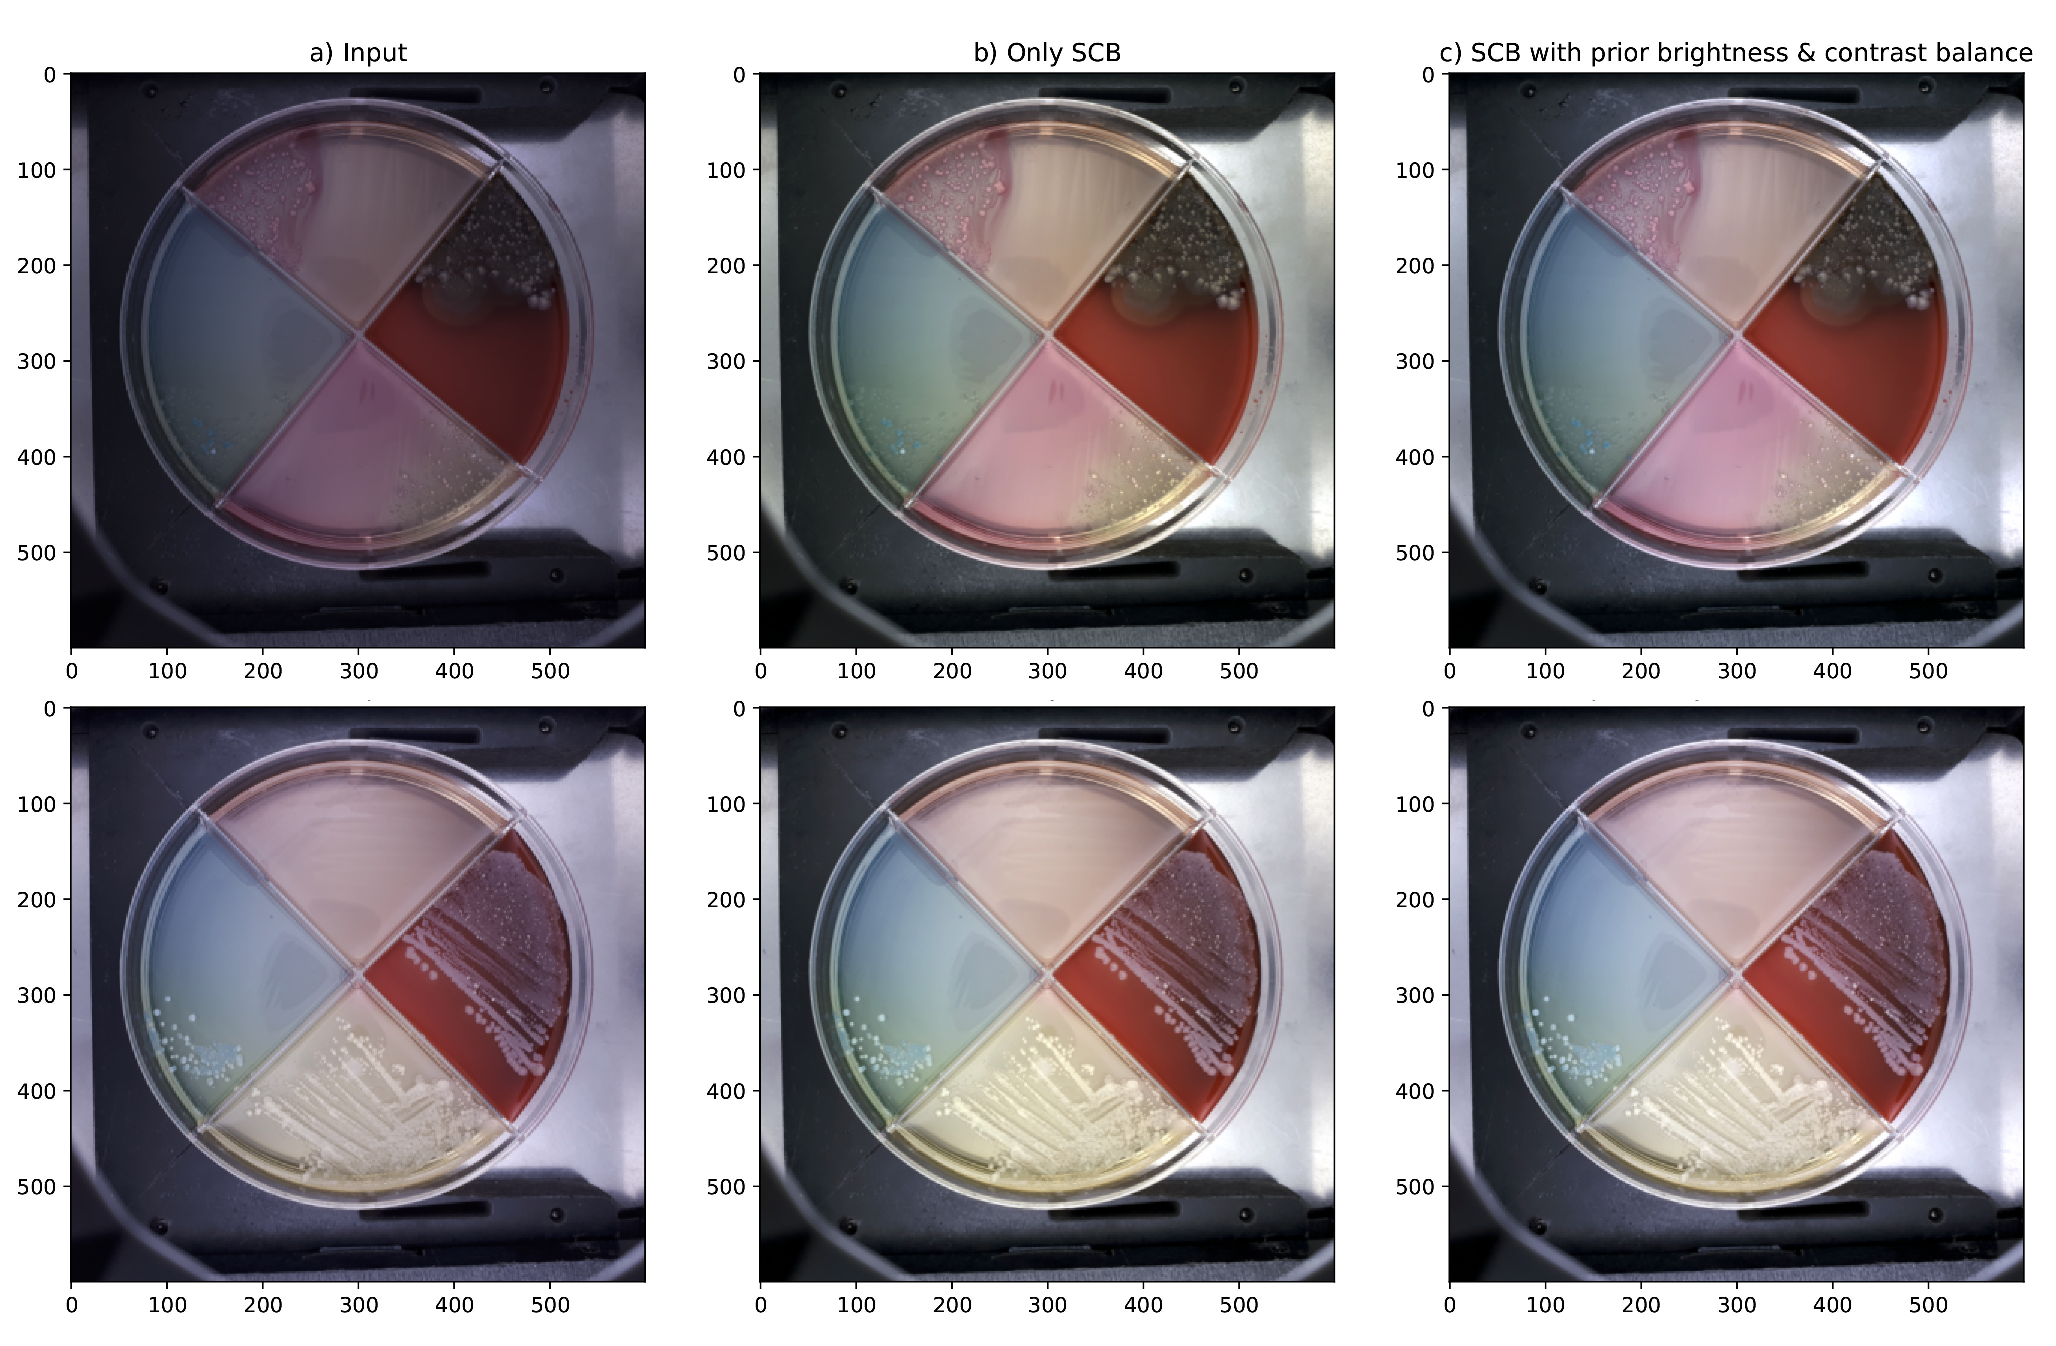
\includegraphics[width=1\linewidth]{figures/PDF/SCB.pdf}\\  
    \caption{a) Input image of an agar plate under dark conditions. b) Image processed with SCB. c) Image processed with SCB with prior brightness and contrast balance  }
    \label{fig:result color balance}
\end{figure}


\noindent As seen in \textit{Figure \ref{fig:result canny}}, Canny proves to be a useful tool for initial edge detection. Adding another iteration of Gaussian blur before Canny, gave a significant improvement in terms of removing image noise such as bacteria clusters and highlighting the actual structure of the agar plate. The result throughout the dataset was mainly dependent on the extent of bacterial growth. Some more extreme cases may have caused the agar plate contour to be connected to features in the background. However, these deviations were later addressed using RANSAC at the end of this section. For this work, the lower and upper threshold values for Canny were set 0, respectively 255, to keep only the most intense pixels. The Gaussian blur sigma value was set to 0.8.

\begin{figure}[H]
    \centering
     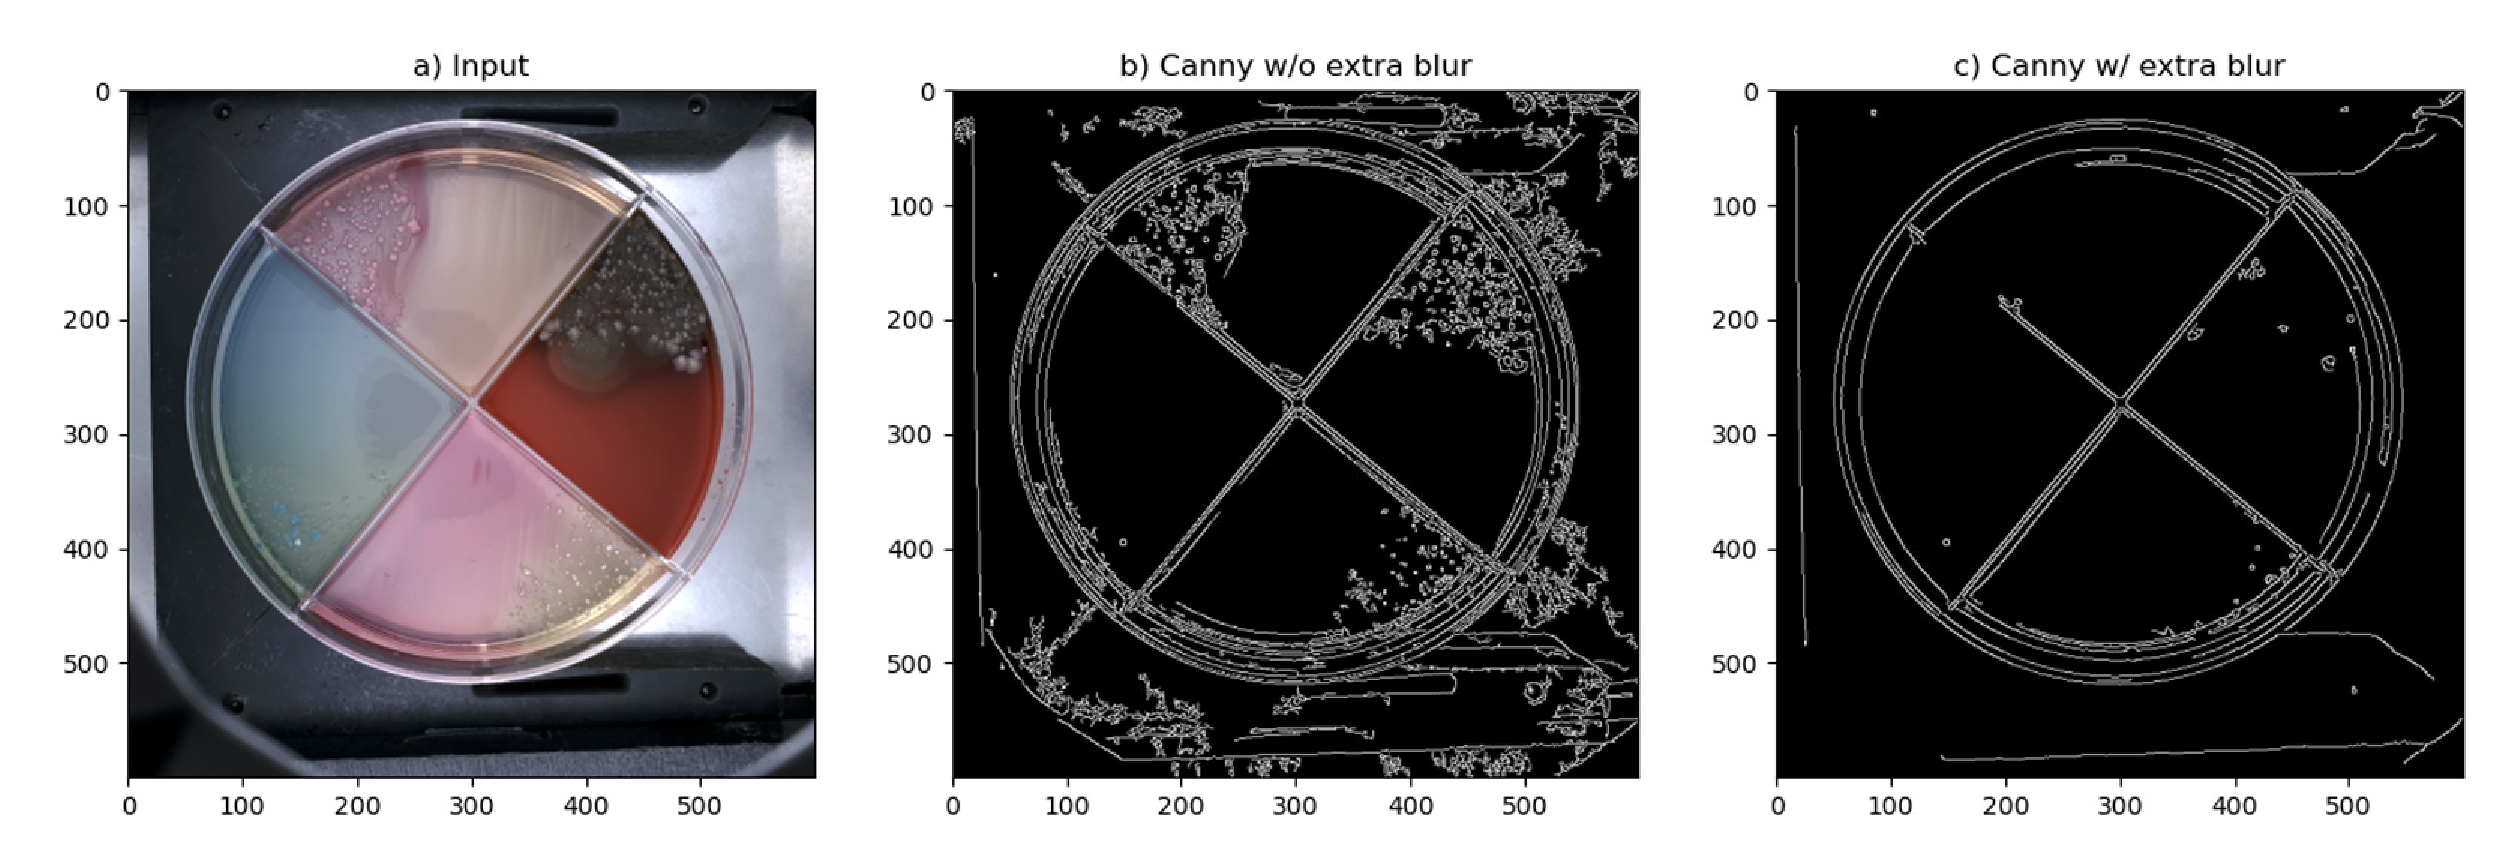
\includegraphics[width=1\linewidth]{figures/PDF/Canny.pdf}\\
    \caption{a) Input image. b) image processed with Canny Edge Detection. c) Image processed with Canny Edge Detection but, with extra Gaussian Blur. }
    \label{fig:result canny}
\end{figure}


\noindent\textit{Figure \ref{fig:result ransac}} shows that RANSAC effectively improves the approximation of the outer contour in deviances occurring during border following. \textit{Figure \ref{fig:result ransac} b)} shows the deviances occurring with Border Following. Closing was made with five iterations of dilation, followed by six iterations of erosion, giving a consistent output for the RANSAC to correct. The sixth iteration of erosion proved useful to remove additional background noise. \\

\noindent Using closing on the Canny output in \textit{Figure \ref{fig:result canny} c)}, the outermost edges could be merged, forming one thick edge, thus providing a more distinctive outer edge, as seen in \textit{Figure \ref{fig:result ransac} a)}.\\

\noindent The found contour was validated with an $ 80\%$ matching rate to their corresponding CHT shape. The matching rate was set a bit lower to cope with the more extreme cases. Images with a matching rate of over $ 85\%$, in this case, proved in general to provide the most accurate results.\\

\noindent RANSAC was set to 100 iterations, which gave accurate results with providing the elliptical contour, as seen in \textit{Figure \ref{fig:result ransac} c)}. However, it was quite time-consuming with a computation time of up to 50 seconds.


\begin{figure}[H]
    \centering
     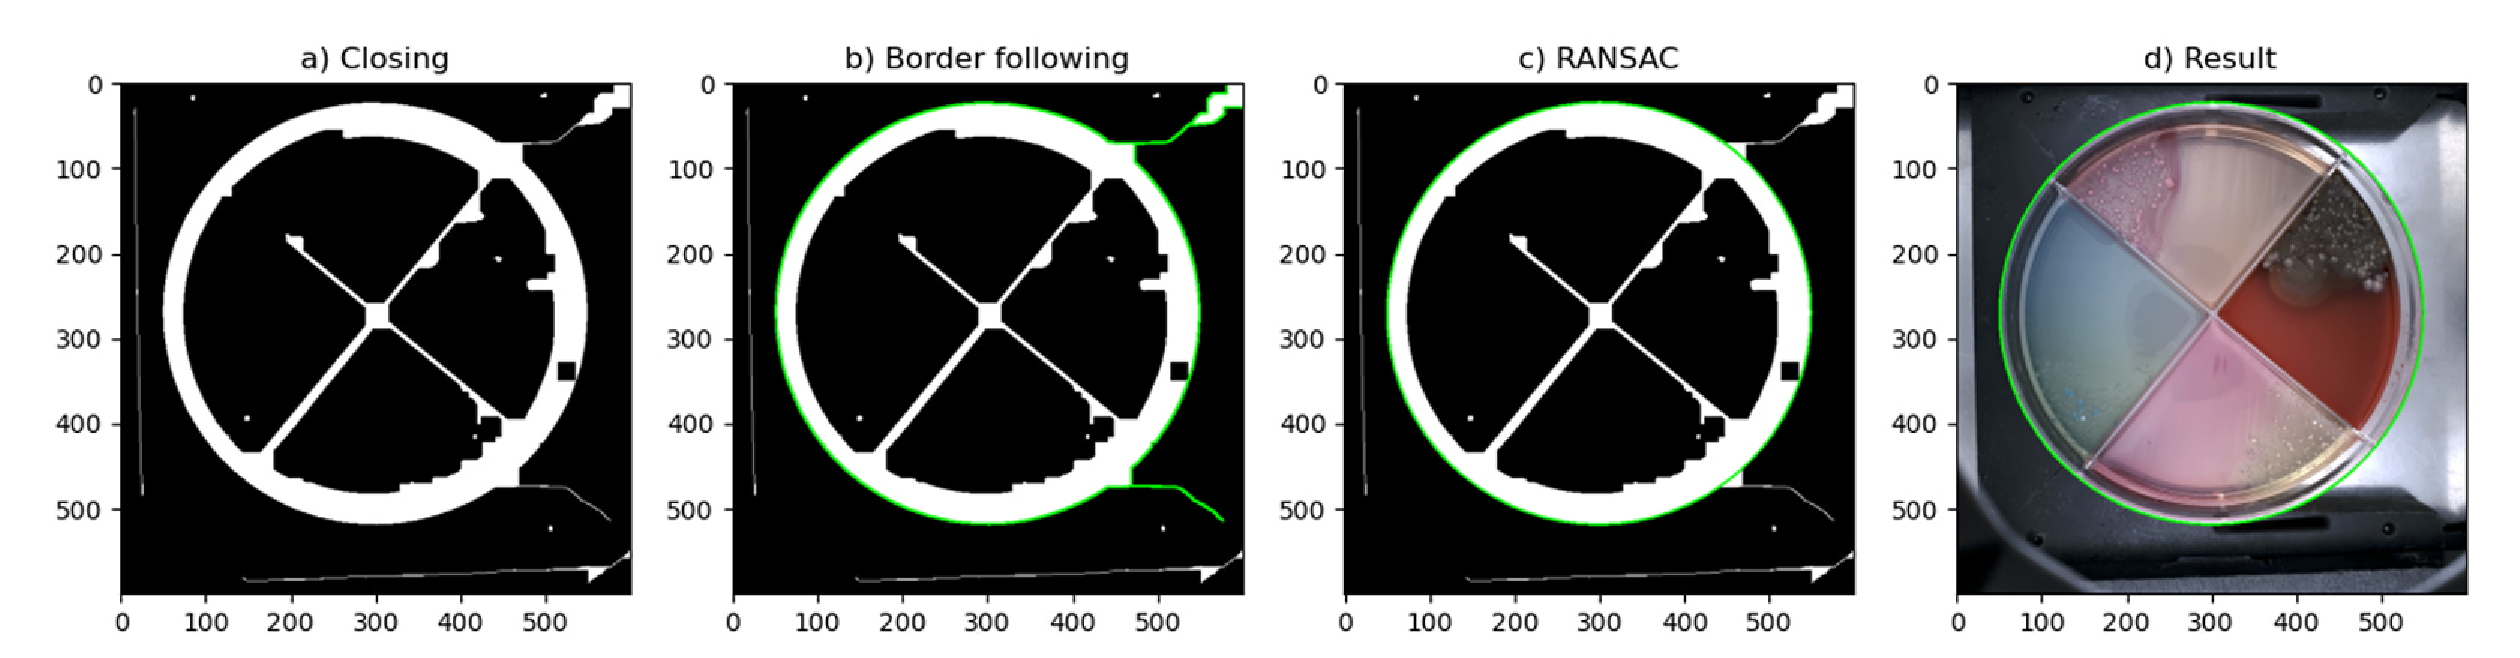
\includegraphics[width=1\linewidth]{figures/PDF/Ransac.pdf}\\
    \caption{a) Closing applied to fix broken canny edges. b) Border following of the outermost contour. c) RANSAC to fit an ellipse on the identified outer edge. d) The final contour of the agar plate identified.}
    \label{fig:result ransac}
\end{figure}

%\noindent Lastly the ROI masking was made using the elliptical contour extracted from the RANSAC, which gave good results as seen in \textit{Figure \ref{fig:result mask})}
%\begin{figure}[H]
%    \centering
%      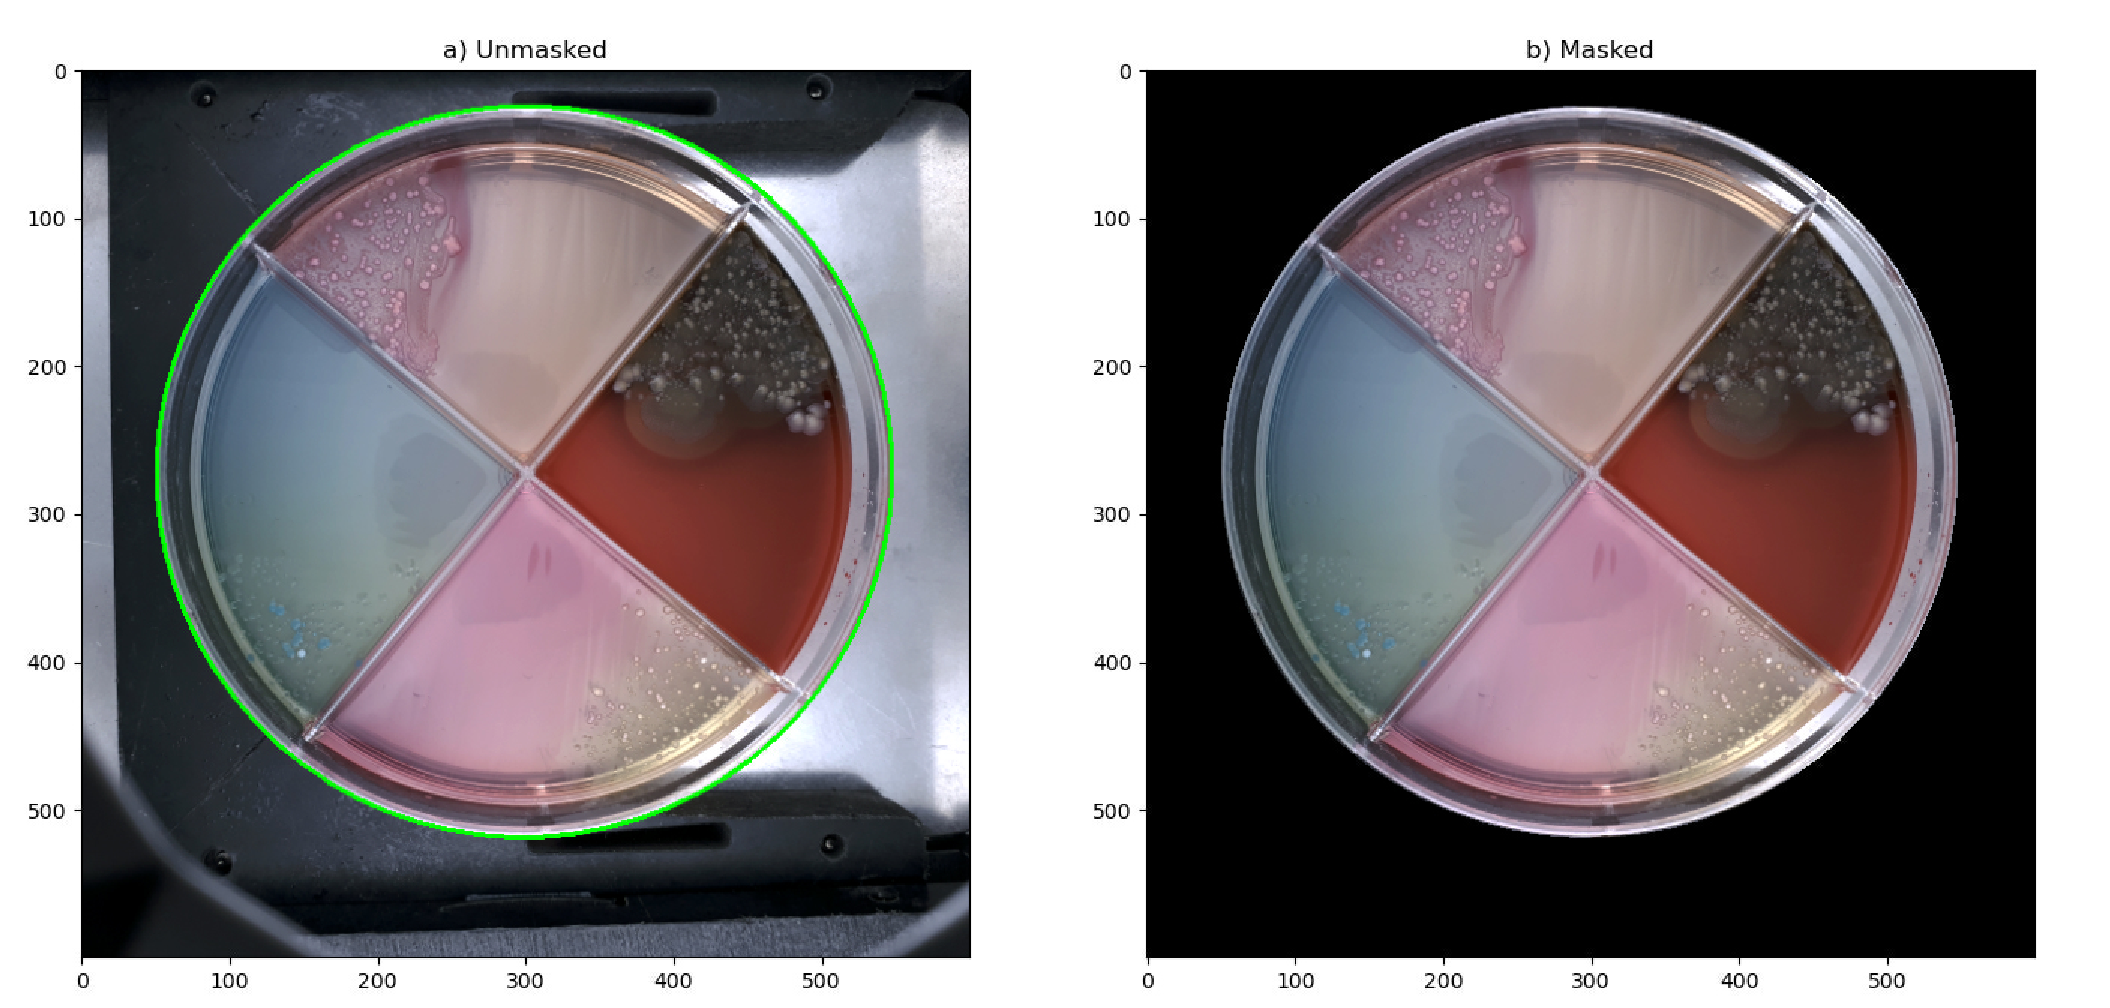
\includegraphics[width=1\linewidth]{figures/PDF/Mask.pdf}\\
%    \caption{a) Agar plate with detected outer contour. b) Pixels outside the outer contour masked . }
%    \label{fig:result mask}
%\end{figure}


\subsection{Identify compartment edges}
Canny, together with the additional Gaussian blur, proved to be an efficient method for identifying the compartment edges. The Gaussian blur sigma value was set to 1.2, a bit higher as opposed to the value in \textit{Section 5.1.1.} Canny, however, operated with the same lower and upper threshold values as before. As a consequence of bacteria clusters growing close to the compartment edges, some edges could not be identified properly, which resulted in some deviations, as seen in the second row of \text{Figure \ref{fig:result skeletonize} a)}.\\

\noindent Morphological Closing gave accurate results in merging any lines, as seen in \textit{Figure \ref{fig:result skeletonize} b)}. However, bacteria clusters close to the compartment edges did sometimes interfere with the edge, as in the second row of \textit{Figure \ref{fig:result skeletonize} b)}. \\

\noindent Lastly, the first row in \textit{Figure \ref{fig:result skeletonize} c)} shows that Skeletonization produced an accurate representation of the centermost edge in \textit{Figure \ref{fig:result skeletonize} b)}, while the input in the second row was affected by bacteria growing close to the edges. However, fairly accurate final results of finding the compartment edges were produced in both cases in \textit{Figure \ref{fig:result houghlines}}, due to the validation.


\begin{figure}[H]
    \centering
      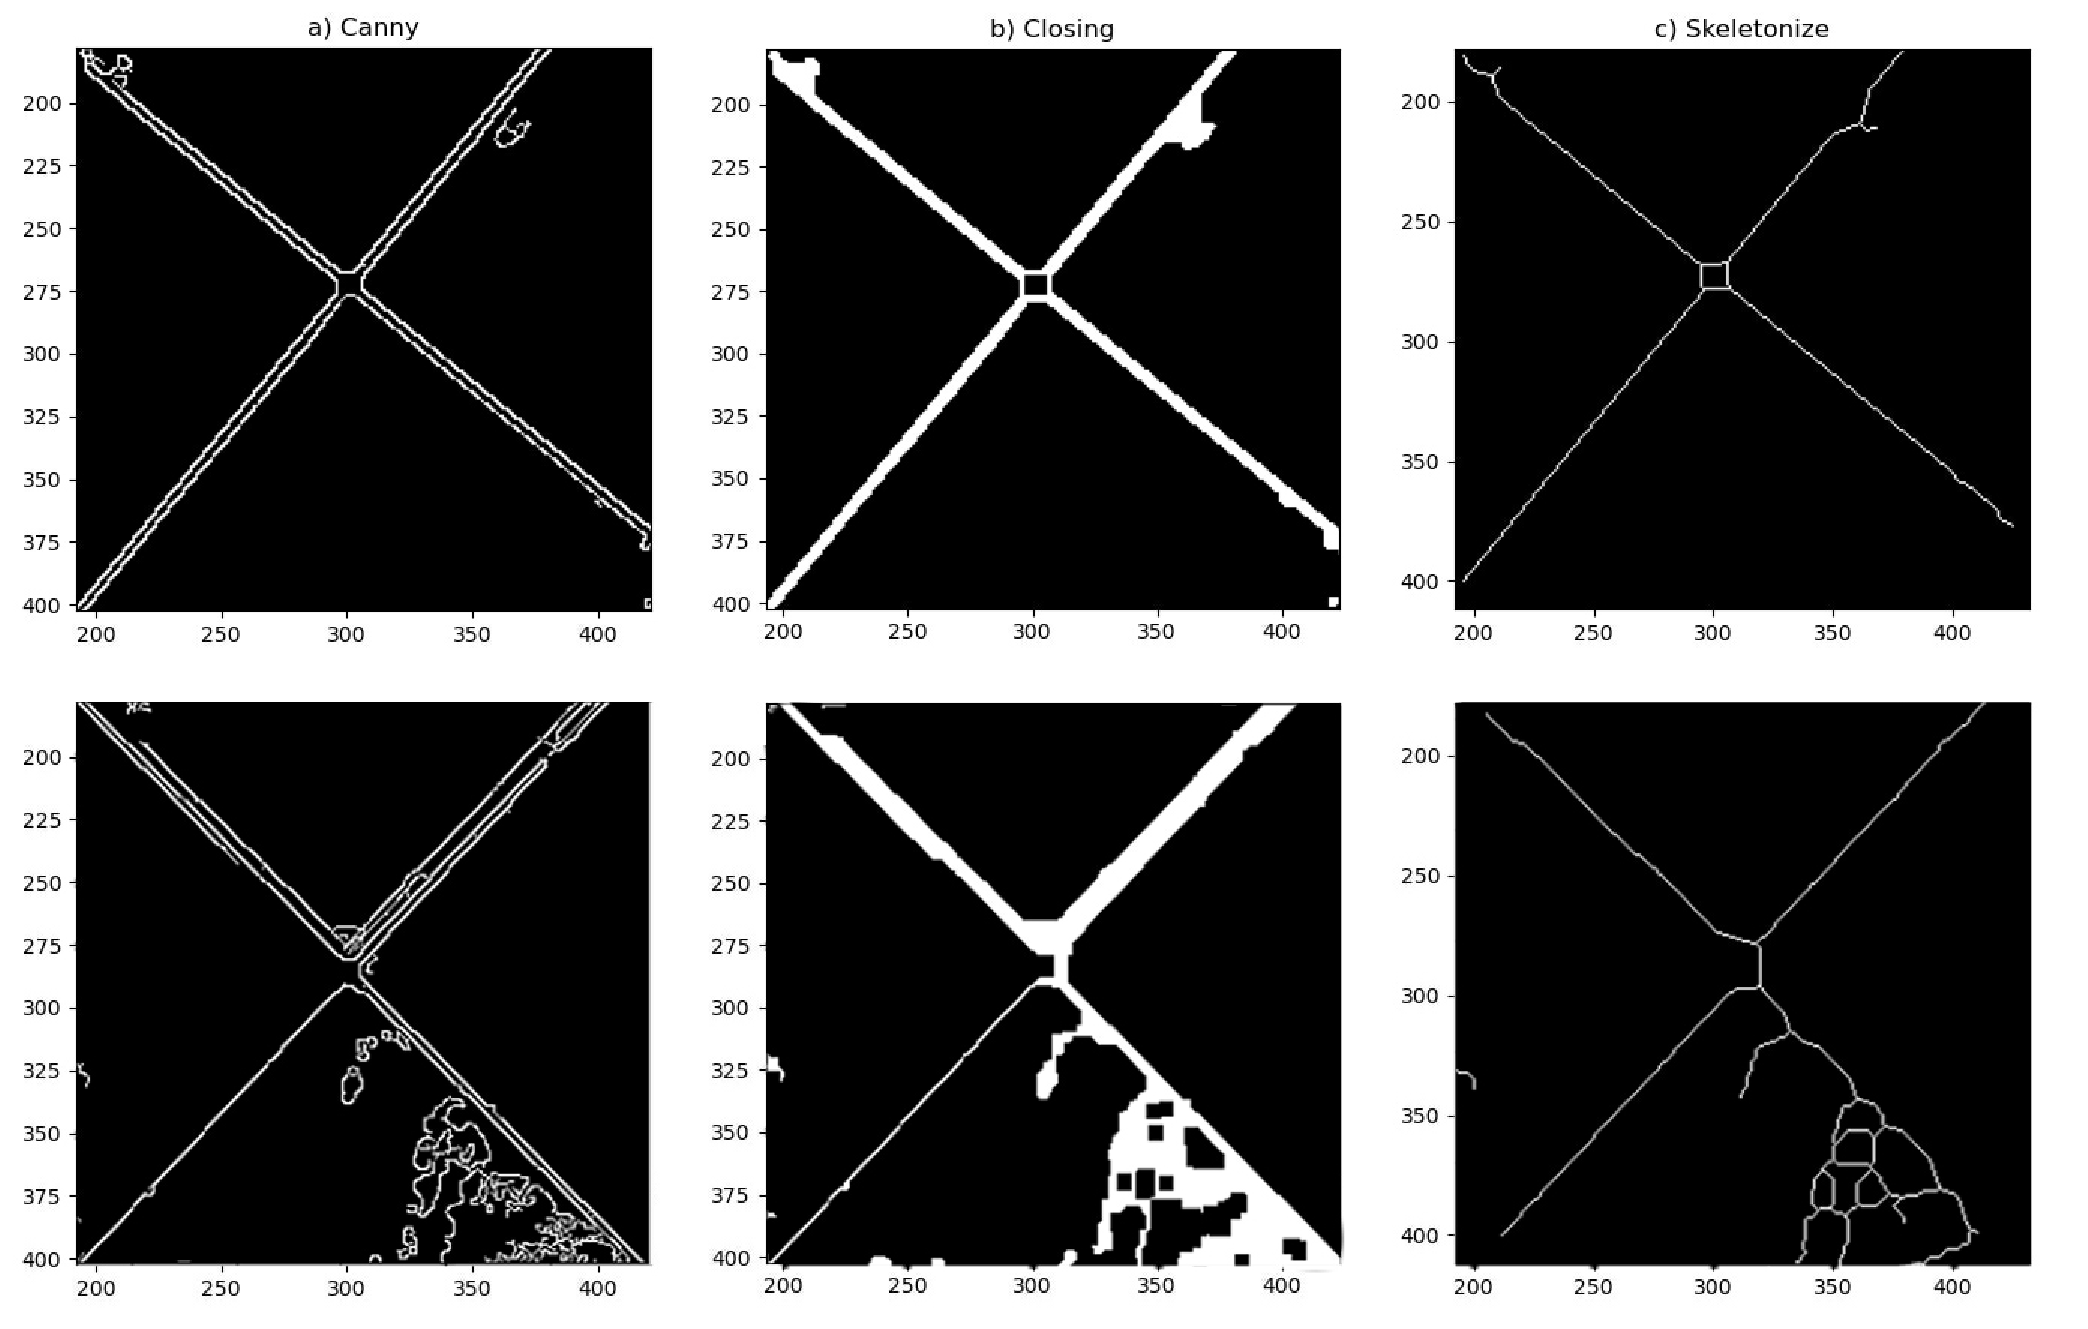
\includegraphics[width=1\linewidth]{figures/PDF/Skeletonize_double.pdf}\\
    \caption{a) Masked binary Canny image. b) Morphological Closing to form one thick line. c) Skeletonize of the thick line, giving a pixel-wide centerline.}
    \label{fig:result skeletonize}
\end{figure}


\begin{figure}[H]
    \centering
      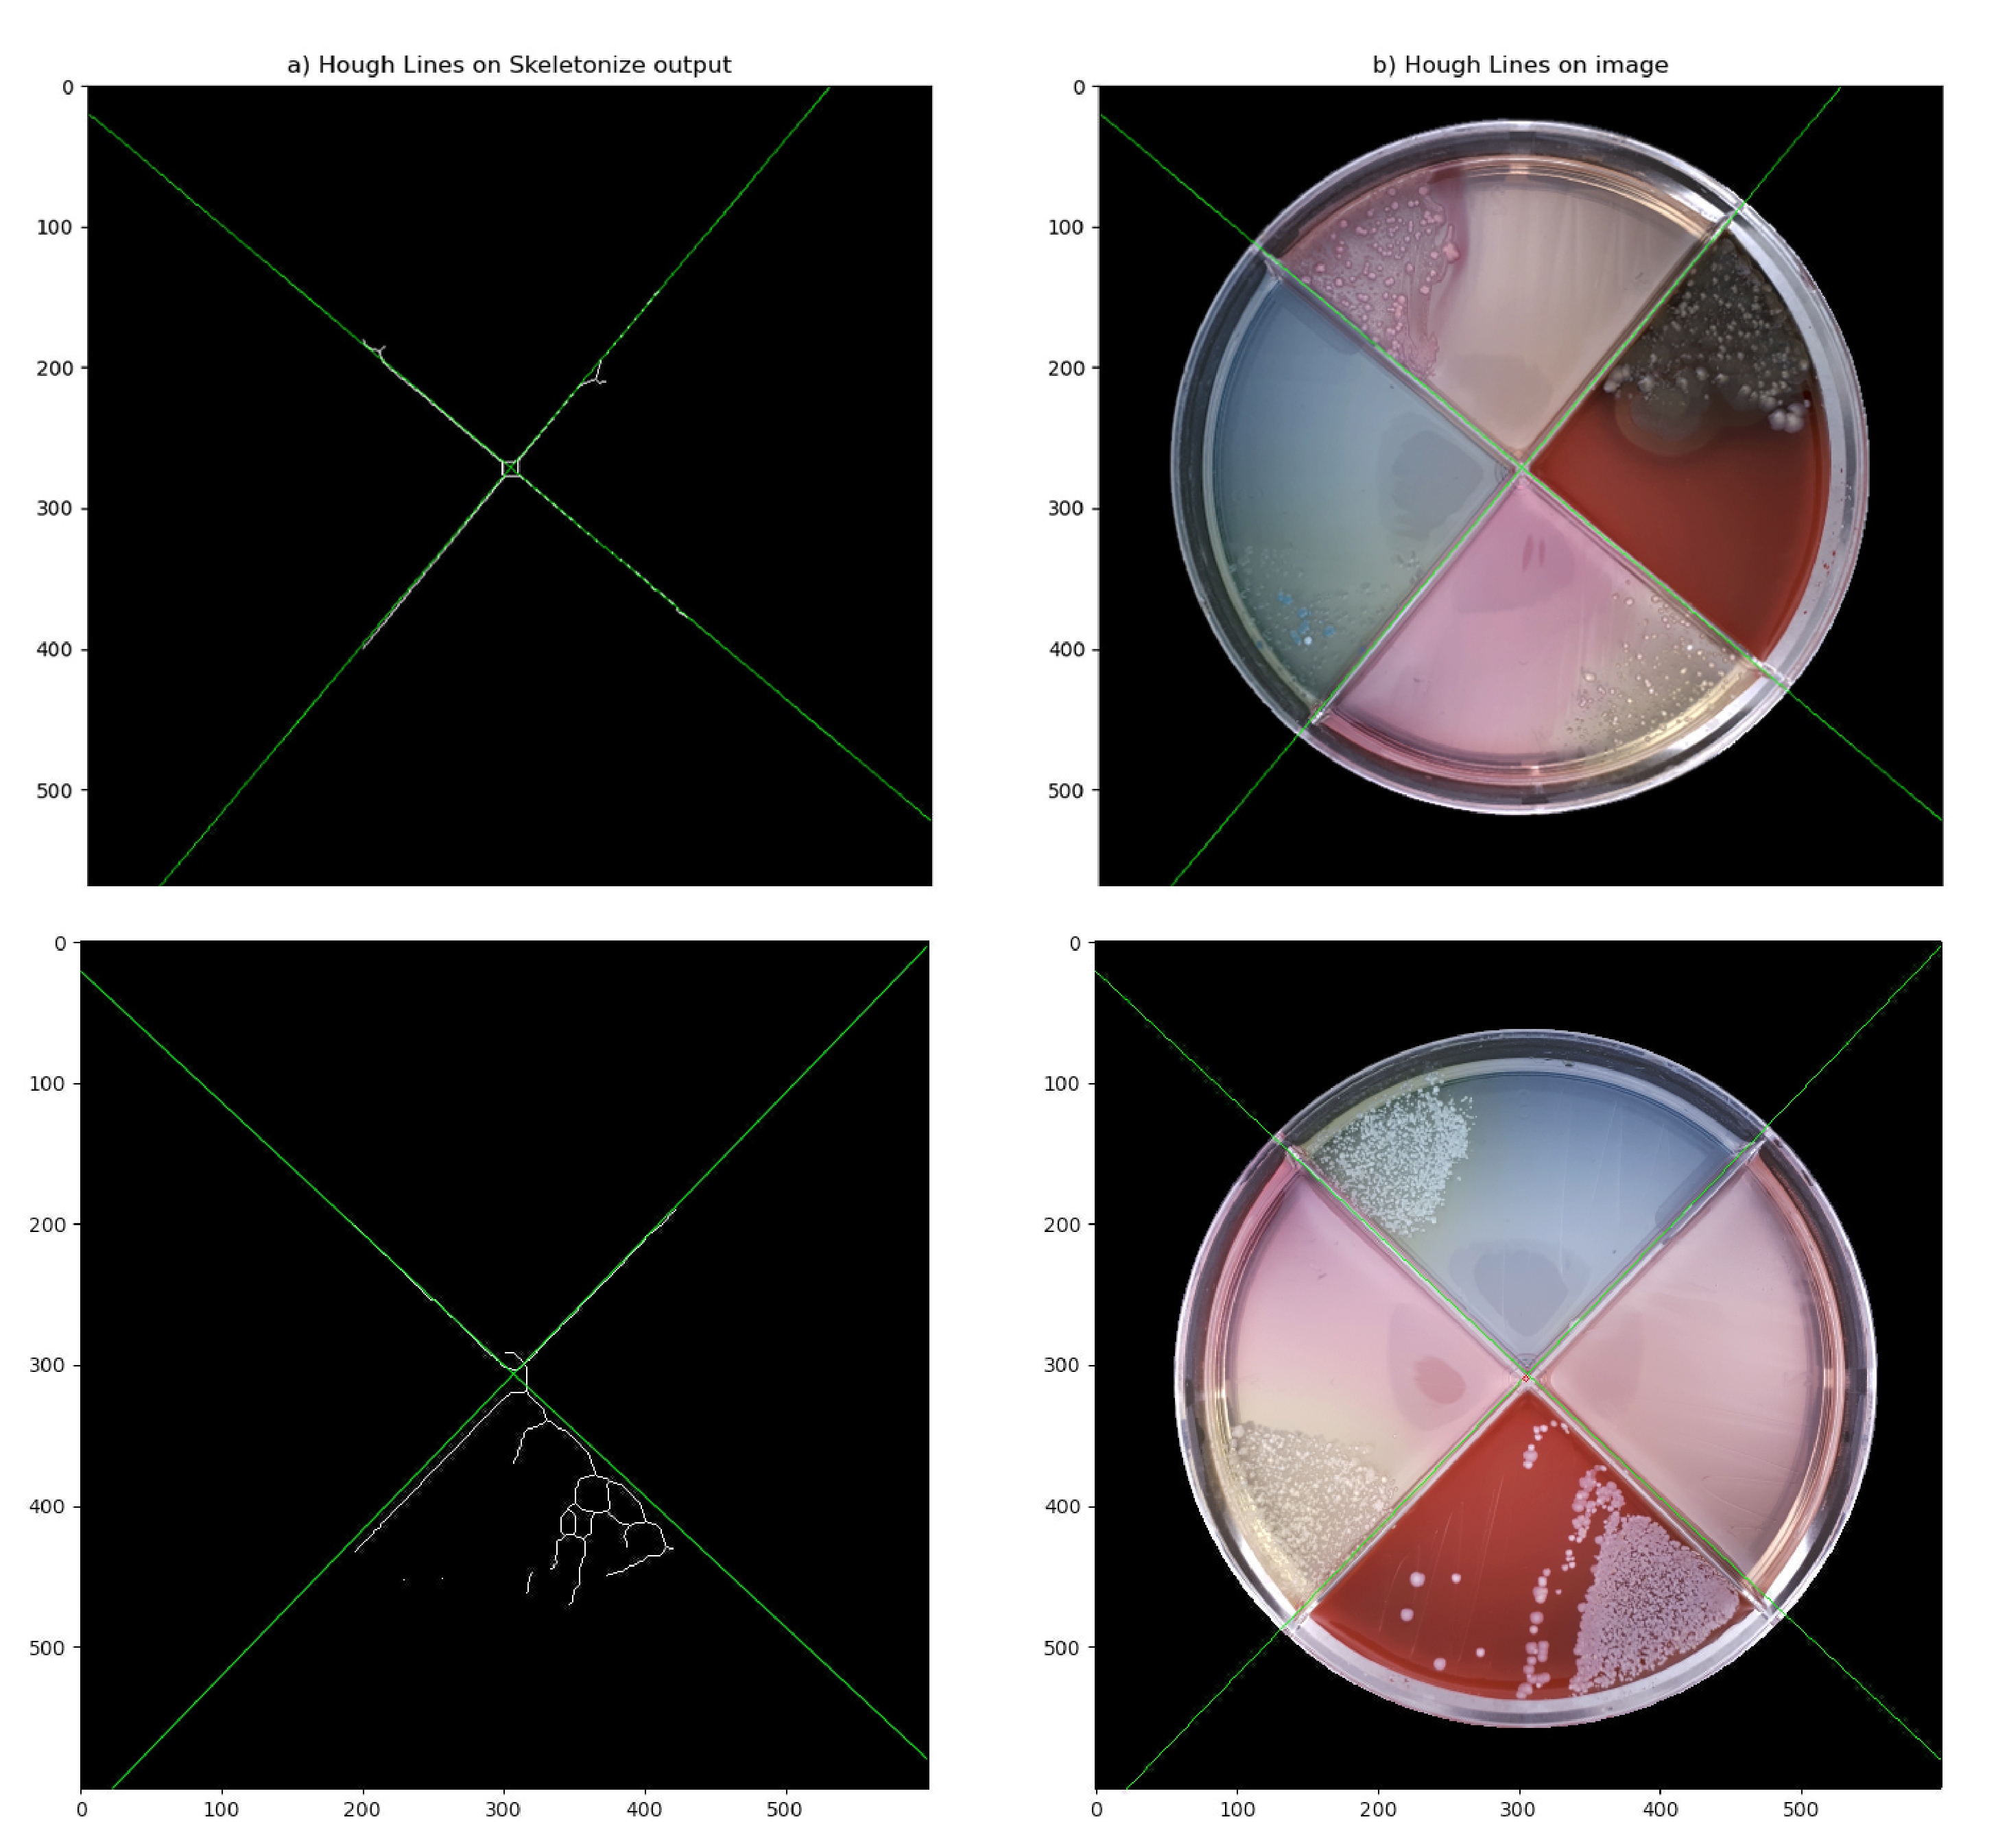
\includegraphics[width=.81\linewidth]{figures/PDF/Hough_lines_double.pdf}\\
    \caption{a) Lines found by Hough Lines over skeletonized output. b) The same lines are drawn over the input image.}
    \label{fig:result houghlines}
\end{figure}

\subsection{Identify agar plate orientation}
Changing the values within the HSV-space gave the most distinctive segmentation of any red pixels. HSV-values were selected to work for the whole dataset, which gave a lower threshold of [H = 0, S = 130, V = 0] and a upper threshold of [H = 179, S = 255, V = 255] to segment the red compartment (see \textit{Figure \ref{fig:result segmentation} b)}). Calculating the red RGB mean value of each line to identify the orientation proved to give consistent results. In many cases, it even worked without the segmentation. However, the segmentation was needed to give accurate results on the entire dataset. With the segmentation of the red compartment, the orientation could easily be identified, as seen in \textit{Figure \ref{fig:result segmentation} c)}. 

\begin{figure}[H]
    \centering
      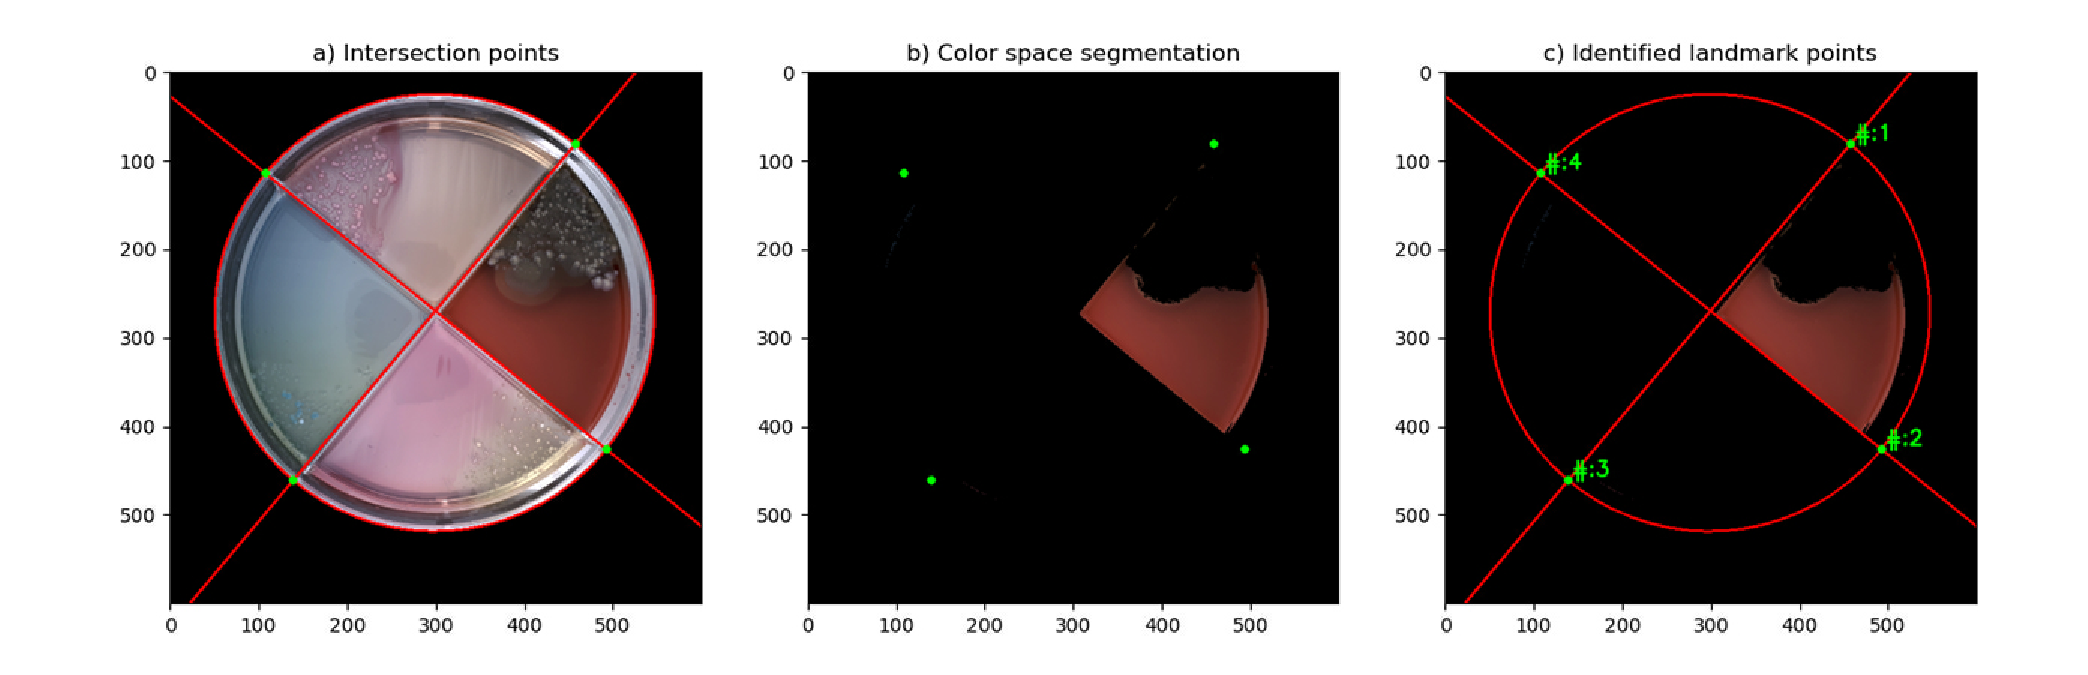
\includegraphics[width=1\linewidth]{figures/PDF/Segmentation.pdf}\\
    \caption{a) Intersection points between the outer contour and the identified compartment edges. b) Segmented red compartment using color space segmentation. c) Sorted intersection points. }
    \label{fig:result segmentation}
\end{figure}

\subsection{Image registration}
As seen in \textit{Figure \ref{fig:result keys} a)}, key points were able to be matched to their corresponding reference points in \textit{Figure \ref{fig:result keys} b)}. The figure, however, only shows a total of 37 key points for illustrational purposes. The final outputs in \textit{Figure \ref{fig:result final} d)} were processed with a total of 10 005 key points, divided into 2 500 key points per line, 5 000 for the ellipse, and 5 for the center and landmark points.\\  

\begin{figure}[H]
      \centering
      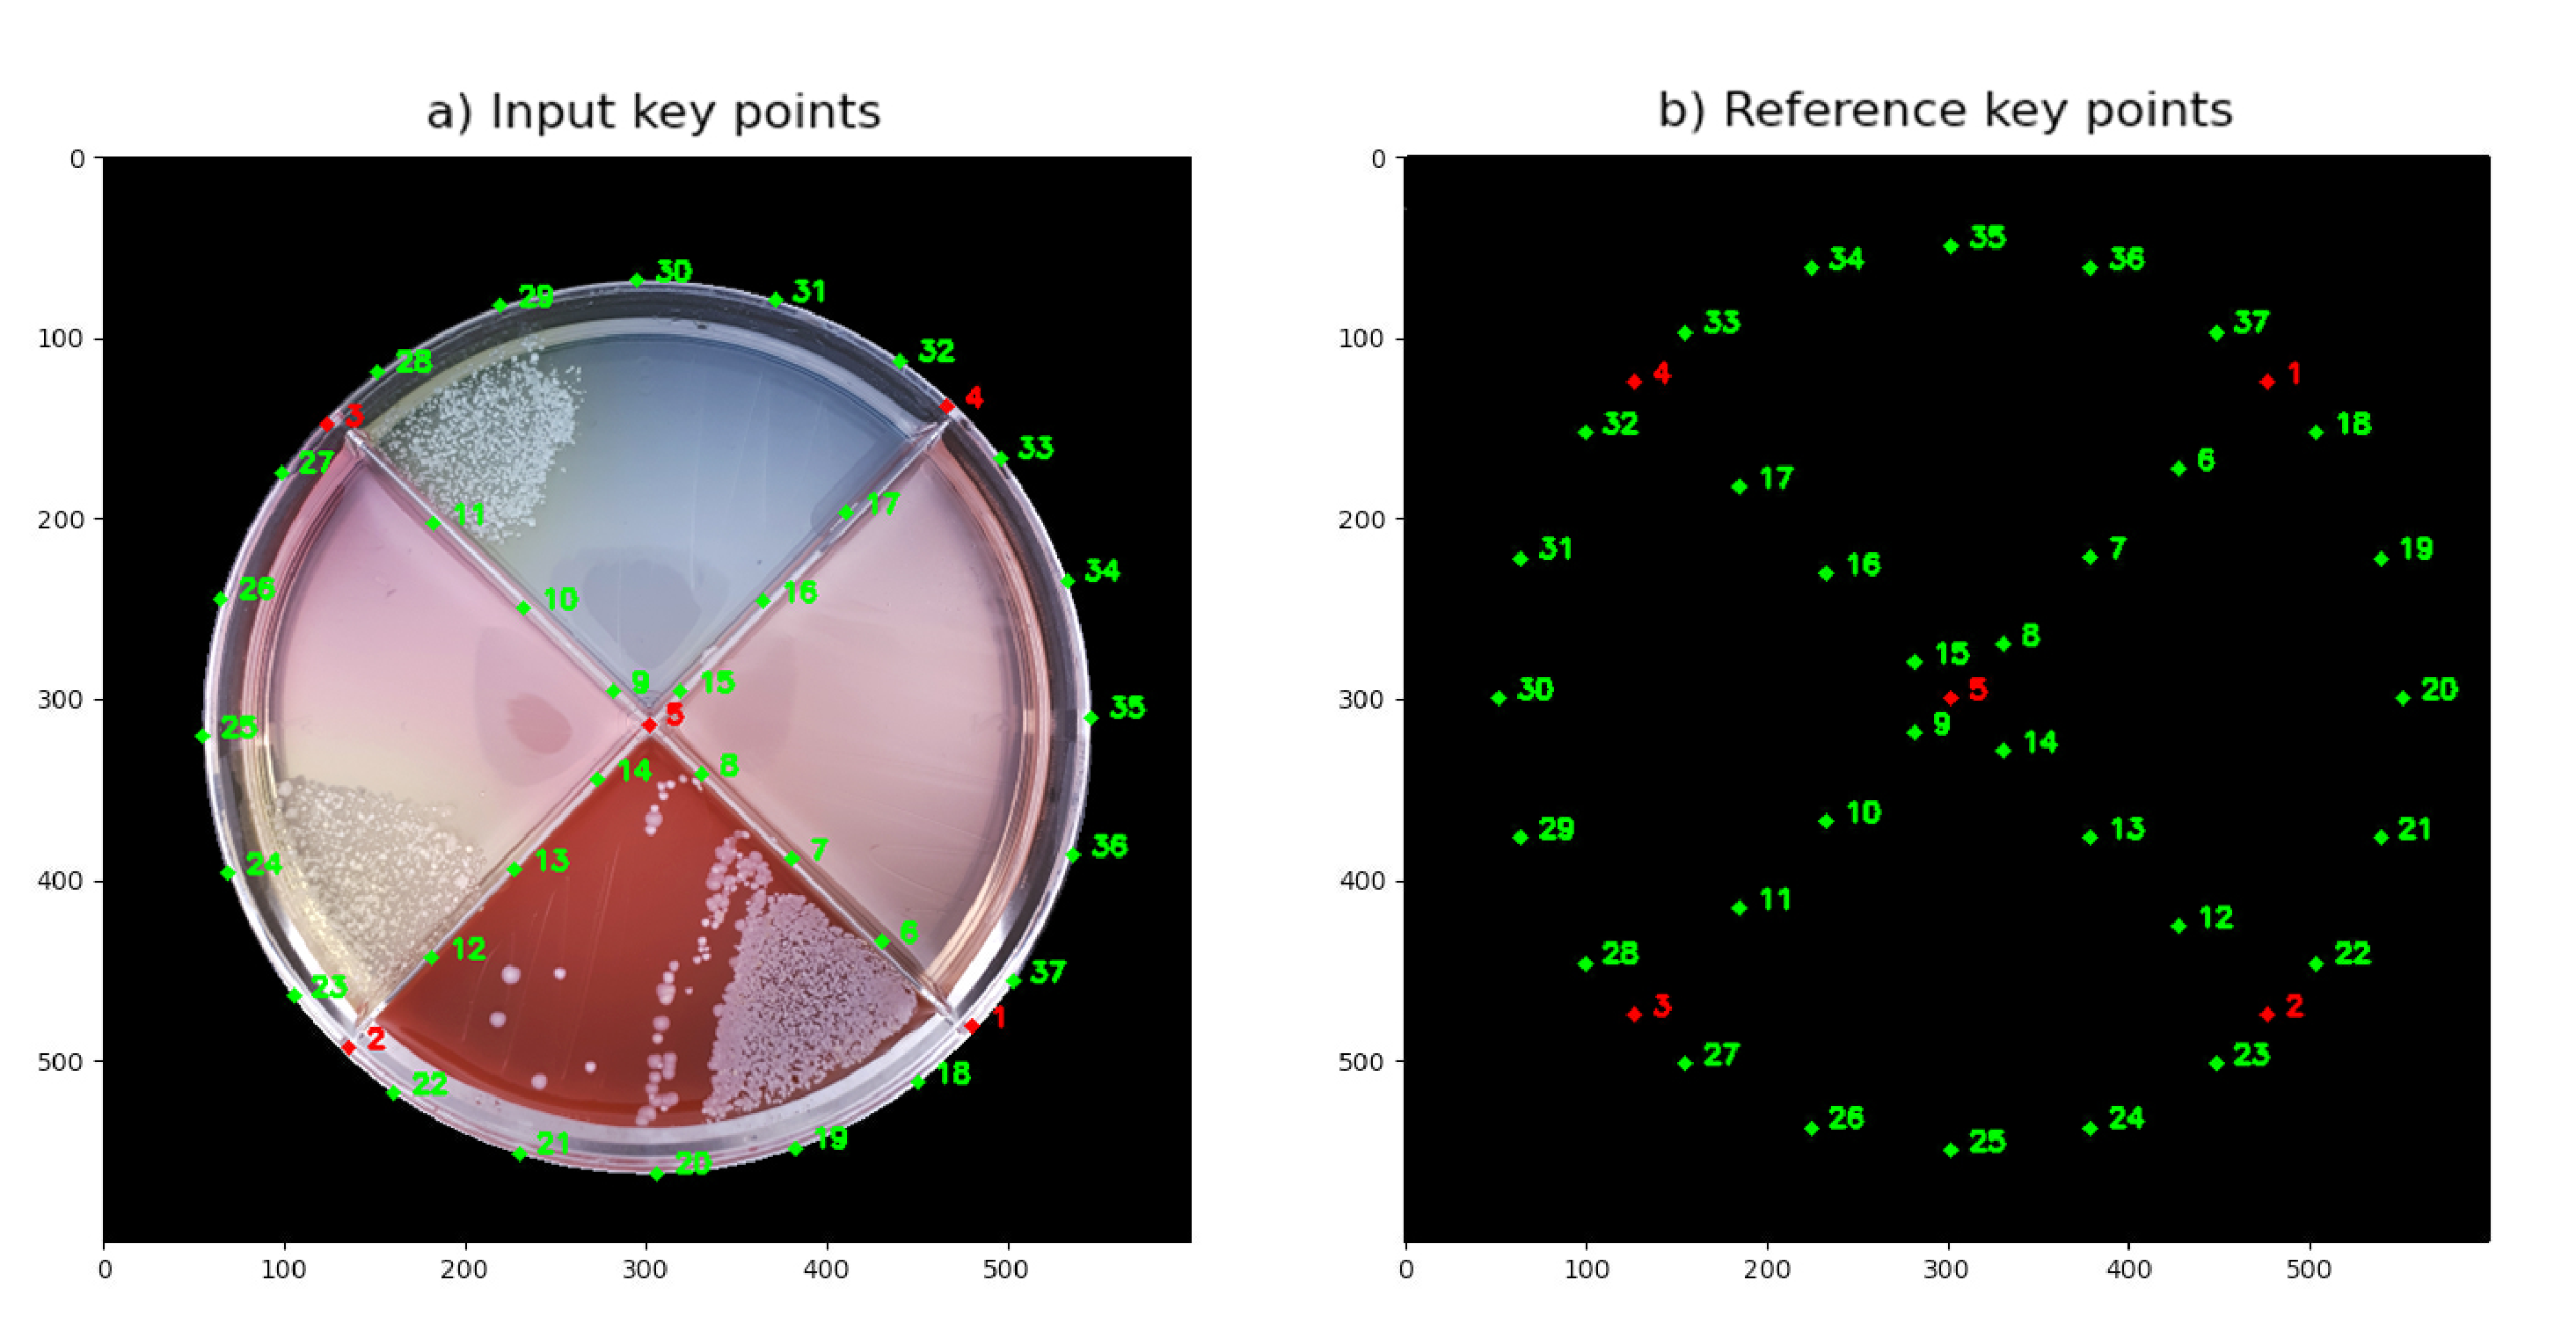
\includegraphics[width=1\linewidth]{figures/PDF/Image_reg.pdf}
    \caption{a) Identified key points for the input image. b) Reference key points.}
    \label{fig:result keys}
\end{figure}

\noindent Finally, \textit{Figure \ref{fig:result projection}} shows very promising results for any perspective distortion still occurring after the first full iteration. A second iteration provided a near-perfect, circular projection of the agar plate. 

\begin{figure}[H]
      \centering
      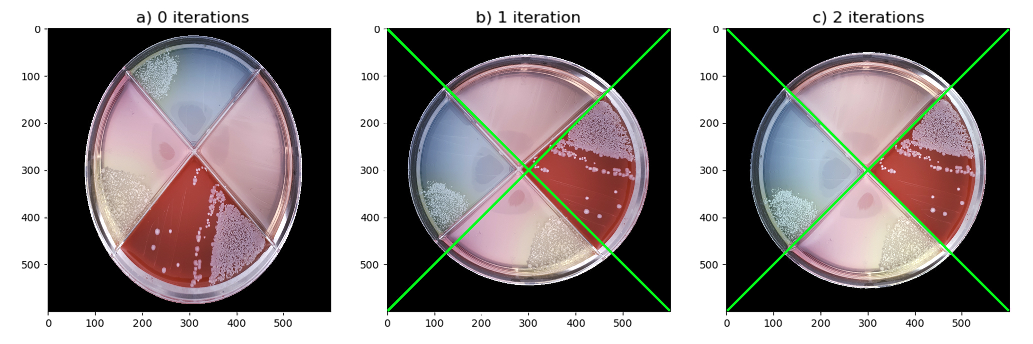
\includegraphics[width=1.1\linewidth]{figures/PDF/Projection.pdf}
    \caption{a) Image constructed with extreme perspective distortion before registration.  b) The result after one iteration. c) The result after two iterations.}
    \label{fig:result projection}
\end{figure}


\section{Evaluation}
 \textit{Figure \ref{fig:result final}} in each step shows that the criteria in \textit{Section 1.3} are met. Therefore, the thesis statement is answered. How the implementation fulfills the criteria can be shown in \textit{Figure \ref{fig:result final}} as follows: 
 \begin{itemize}
     \item \textit{The outer edge of the agar plate shall be identified. The compartment edges shall be identified as well. }
 \end{itemize}
\textit{Figure \ref{fig:result final} b)} shows that Canny, Morphological Closing, Border Following, and RANSAC were successful in providing an elliptical shape around the outer contour of an agar plate. \textit{Figure \ref{fig:result final} c)} shows that the compartment edges can be identified using Canny, Morphological Closing, Skeletonize, and Hough Transform. 
  \begin{itemize}
     \item \textit{Pixels outside the agar plate should be masked to remove background noise.}
 \end{itemize}
 As seen in \textit{Figure \ref{fig:result final} c)}, masking proved to be consistent and any relevant noise is masked if, the outer contour of the agar plate is identified correctly.
 \textit{Figure \ref{fig:result final} c)}.. 
  \begin{itemize}
     \item \textit{Depending on the angle, position, and scale, the image should be adjusted to match a reference image.}
 \end{itemize}
 \textit{Figure \ref{fig:result final} d)} shows the input image in \textit{Figure \ref{fig:result final} a)} is adjusted in scale, position, perspective, and rotation based on a reference image.




%%%%%%%%%%%%%%%%%%%%%%%%%%%%%%%%%%%%%%%%%%%%%%%%%%%%%%%%%%%%%%%%%%%%%%
%%% lorem.tex ends here

%%% Local Variables: 
%%% mode: latex
%%% TeX-master: "demothesis"
%%% End: 

%%% lorem.tex --- 
%% 
%% Filename: lorem.tex
%% Description: 
%% Author: Ola Leifler
%% Maintainer: 
%% Created: Wed Nov 10 09:59:23 2010 (CET)
%% Version: $Id$
%% Version: 
%% Last-Updated: Wed Nov 10 09:59:47 2010 (CET)
%%           By: Ola Leifler
%%     Update #: 2
%% URL: 
%% Keywords: 
%% Compatibility: 
%% 
%%%%%%%%%%%%%%%%%%%%%%%%%%%%%%%%%%%%%%%%%%%%%%%%%%%%%%%%%%%%%%%%%%%%%%
%% 
%%% Commentary: 
%% 
%% 
%% 
%%%%%%%%%%%%%%%%%%%%%%%%%%%%%%%%%%%%%%%%%%%%%%%%%%%%%%%%%%%%%%%%%%%%%%
%% 
%%% Change log:
%% 
%% 
%% RCS $Log$
%%%%%%%%%%%%%%%%%%%%%%%%%%%%%%%%%%%%%%%%%%%%%%%%%%%%%%%%%%%%%%%%%%%%%%
%% 
%%% Code:

\chapter{Discussion}
\label{cha:discussion}
This chapter discusses and analyzes the results and methods derived from the previous chapters. Additionally, the work will be put in a wider context. 

\section{Results}
\label{sec:discussion-results}
Overall the results look promising, with only some minor variations in perspective and rotation (see examples in \textit{Figure \ref{fig:result final} d)}). The biggest reason for any output variations seems to be deviations when finding the compartment edges, essentially due to the extent of bacteria occurring, as well as their positioning. While \textit{Figure \ref{fig:result final} b)} shows nearly identical results,  \textit{Figure \ref{fig:result final} c)} shows slight variations in the positioning and angle of the identified edges. \\

\noindent Using Canny with the additional blur seems to be a promising way to cope with any noise from bacteria growth. Very accurate final results were possible to produce when slightly adjusting the parameters of Dilate, Erosion, Canny, and Gaussian blur individually for each image. However, parameters were set to work with the whole dataset to provide a more generally applicable solution to the thesis problem. \\

\noindent The fact that the agar plate is circular, and not dependent on the background made it much more difficult to identify its orientation.  Usually, some landmark points in corners, shapes, or the background can be found, but here a color segmentation was needed as an addition to defining the rotation. \\

\section{Method}
\label{sec:discussion-method}

The method proved to work, thus leading to good results, but could mainly be improved in some aspects. \\

\noindent For example, additional validation of the Canny output in \textit{Figure \ref{fig:compartment edges flowchart}} could be implemented to validate that the compartment edges are identified, as shown in \textit{Figure \ref{fig:compartment masking} b)}. Either the contrast and brightness could be adjusted as during the validation in \textit{Figure \ref{fig:identify and mask flowchart}}; alternatively the Gaussian blur sigma adjusted depending on the situation. If this were to be successful in all cases, the Closing and Skeletonize would not be needed. Instead, the centermost part of the compartment edges could be simply calculated from the four edges identified. \\

\noindent Even though using RANSAC increased the accuracy of identifying the agar plate, it proved to be very computationally expensive. However, the number of RANSAC iterations was a consequence of using parameters suitable enough for the whole dataset and could be lowered if the pre-processing was optimized. For application areas that are dependent on faster computation speed, CHT alone could be used to replace the whole \texit{Section 5.1.1.}, still producing good-enough results in cases with little to no perspective distortion.\\

\noindent Instead of processing each output multiple times, any perspective distortion could be directly calculated with the major and minor axis of the circular projection of the agar plate. The major and minor axis should then correspond to the compartment edges and the contour found in \texit{Section 4.1.1}. Ideally, this operation would reduce the need to only a single processing iteration.




\item 
\section{The work in a wider context}
\label{sec:work-wider-context}
Imagining the social and ethical aspects of image processing is difficult. However, using image processing to pre-process images before being used by a bacteria classifier improves the possibility of correctly identifying the right type of bacteria. Therefore, this work could be a base to improve the input used for all types of automated bacteria classifiers using agar plates. Improving the results of automated bacteria classifiers can not only for mastitis, improve the time-consuming and lengthy diagnosis process. \\
%Öppnar upp portar för bakterie klassifierare
%knytt ihop säcken med det som skrevs i börja av introduktionen
 
%This work could be a base for all types of bacteria classifications. Improving the input images used by bacteria classifiers 


%\item The work could be a base for all type of bacteria classification using agar plates. It is not just limited to mastitis. 
%Talk about the ethical and social aspects related to the work. Here write about the social and ethical aspects of mastitis and its contribution to the use of antibiotics? (Maybe??)

%%%%%%%%%%%%%%%%%%%%%%%%%%%%%%%%%%%%%%%%%%%%%%%%%%%%%%%%%%%%%%%%%%%%%%
%%% lorem.tex ends here

%%% Local Variables: 
%%% mode: latex
%%% TeX-master: "demothesis"
%%% End: 

\twoside
%%% lorem.tex --- 
%% 
%% Filename: lorem.tex
%% Description: 
%% Author: Ola Leifler
%% Maintainer: 
%% Created: Wed Nov 10 09:59:23 2010 (CET)
%% Version: $Id$
%% Version: 
%% Last-Updated: Wed Nov 10 09:59:47 2010 (CET)
%%           By: Ola Leifler
%%     Update #: 2
%% URL: 
%% Keywords: 
%% Compatibility: 
%% 
%%%%%%%%%%%%%%%%%%%%%%%%%%%%%%%%%%%%%%%%%%%%%%%%%%%%%%%%%%%%%%%%%%%%%%
%% 
%%% Commentary: 
%% 
%% 
%% 
%%%%%%%%%%%%%%%%%%%%%%%%%%%%%%%%%%%%%%%%%%%%%%%%%%%%%%%%%%%%%%%%%%%%%%
%% 
%%% Change log:
%% 
%% 
%% RCS $Log$
%%%%%%%%%%%%%%%%%%%%%%%%%%%%%%%%%%%%%%%%%%%%%%%%%%%%%%%%%%%%%%%%%%%%%%
%% 
%%% Code:

\chapter{Conclusion}
\label{cha:conclusion}
In conclusion, a combination of image processing algorithms and techniques were found to answer the problem description. The solution proved to be invariant to scale, perspective, and rotation, which consequently opens up to a wider area of application. \\

\noindent During the research for the thesis, few papers were found with a similar problem description. A substantial amount of previous work has been done by others on edge detection and object identification, which made it possible to construct a good base for this work. \\

\noindent Most of the papers found, dedicated to Image registration, were based on the registration of images picturing the same object but taken under varying conditions. However, the problem description of this thesis addressed the registration of different objects, but of the same type (an agar plate). Therefore, the characteristics of the problem made it necessary to find a more generally applicable approach. \\ 

\noindent The collection of techniques described in this thesis should, besides processing an agar plate, apply to other types of objects as well. Hopefully, it could add some improvement when used in, e.g., bacteria classification or other areas.

\section{Future work}
Future work for this thesis could be as follows: 
\begin{enumerate}
    \item Improving Canny, or finding other methods, that could mask bacteria clusters would improve the accuracy of identifying the compartment edges. 
    \item An implementation to cope with the elliptical projection distortion can be done, so that no more than one iteration of the whole process is needed. 
    \item Improve the accuracy of Canny and Border Following when detecting the outer edge of an agar plate. Improving the accuracy will remove the need for RANSAC thus, improving the computational speed. 
\end{enumerate}


%%%%%%%%%%%%%%%%%%%%%%%%%%%%%%%%%%%%%%%%%%%%%%%%%%%%%%%%%%%%%%%%%%%%%%
%%% lorem.tex ends here

%%% Local Variables: 
%%% mode: latex
%%% TeX-master: "demothesis"
%%% End: 

\printbibliography
\end{document}

%%%%%%%%%%%%%%%%%%%%%%%%%%%%%%%%%%%%%%%%%%%%%%%%%%%%%%%%%%%%%%%%%%%%%%
%%% demothesis.tex ends here

